\documentclass[12pt,twoside]{report}

\usepackage{graphicx}                  % For including graphics
\usepackage{subfigure}                 % For multipart figures
\usepackage{listings}                  % For prettyprinting of source code
\usepackage{color}                     % Color package
\usepackage{amsfonts,amsmath,amssymb}  % Math packages

% Configure hyperref package for PDF output
\usepackage[pdftex,
        colorlinks=true,
        urlcolor=rltblue,              % \href{...}{...} external (URL)
        filecolor=rltgreen,            % \href{...} local file
        linkcolor=rltblue,             % \ref{...} and \pageref{...}
        pdftitle={LLAMAComm Documentation},
        pdfauthor={Derek Young and Adam Margetts},
        pdfsubject={LLAMAComm Documentation},
        pdfkeywords={LLAMAComm, MIMO, documentation, frequency scavenging,
            cognitive, communications},
        pdfproducer={pdfLaTeX},
        pagebackref,
        pdfpagemode=None,
        bookmarksopen=true]{hyperref}
\definecolor{rltred}{rgb}{0.75,0,0}
\definecolor{rltgreen}{rgb}{0,0.5,0}
\definecolor{rltblue}{rgb}{0,0,0.75}

% Object definitions
\newcommand{\node}{{\tt node}}
\newcommand{\module}{{\tt module}}
\newcommand{\env}{{\tt environment}}
\newcommand{\link}{{\tt link}}

% Configure listings package
\lstset{
    language=matlab,                   % Set default language to MATLAB
    basicstyle=\footnotesize\tt,       % print whole listing small and fixed font
    keywordstyle=\color{black},        % control how keywords appear
    identifierstyle=,                  % formatting for variables
    commentstyle=,                     % formatting for comments
    stringstyle=,                      % formatting for strings
    showstringspaces=false,            % turn off special space characters
    numbers=left,                      % Formatting for line numbers
    numberstyle=\tiny,
    stepnumber=2,
    numbersep=10pt,
    backgroundcolor=\color{codegray},  % Puts text into gray box
    aboveskip=10pt,                    % Add blank space above box
    belowskip=10pt                     % Add black space below box
}
\definecolor{codegray}{rgb}{.9,.9,.9}  % Background color for code blocks

% Change formatting of description label
% This affects the description lists in the reference section
\renewcommand{\descriptionlabel}[1]
{\hspace{\labelsep}\texttt{#1}}

%% Configure the page layout
\oddsidemargin 0.25in
\evensidemargin 0in
\textwidth 6.25in

%% INPUT THE HEADER FILE
%------------------------------------------------------------------
%------------------------------------------------------------------
%------------------------------------------------------------------
%------------------------------------------------------------------
{\global\def\putFig#1#2#3{
        \begin{figure}[tp]
           \begin{center}
              \epsfxsize=#3in
              \epsfbox{figures/#1.eps}
           \end{center}
           \caption{\small{#2}}
           \label{fig:#1}
        \end{figure}
        }
} {\global\def\putFrag#1#2#3#4{
        \begin{figure}[tp]
           \begin{center}
              #4
              \epsfxsize=#3in
              \epsfbox{figures/#1.eps}
           \end{center}
           \caption{\small{#2}}
           \label{fig:#1}
        \end{figure}
        }
} {\global\def\twoFig#1#2#3{
        \begin{figure}[tp]
           \begin{center}
              \hfill
              \epsfxsize=2.75in
              \epsfbox{figures/#1.eps}
              \hfill
              \epsfxsize=2.75in
              \epsfbox{figures/#2.eps}
           \end{center}
           \caption{\small{#3}}
           \label{fig:#1}
        \end{figure}
        }
} {\global\def\twoFrag#1#2#3#4{
        \begin{figure}[tp]
           \begin{center}
              #4
              \hfill
              \epsfxsize=2.75in
              \epsfbox{figures/#1.eps}
              \hfill
              \epsfxsize=2.75in
              \epsfbox{figures/#2.eps}
           \end{center}
           \caption{\small{#3}}
           \label{fig:#1}
        \end{figure}
        }
} {\global\def\tempFig#1#2#3{
        \begin{figure}[h]
           \begin{center}
              \framebox[6in]{
                \bigskip
                {\bf Figure will go here.}
                \bigskip
              }
           \end{center}
           \caption{\small{#2}}
           \label{fig:#1}
        \end{figure}
        }
}
%------------------------------------------------------------------

 % math shortcuts
 \newcommand{\defn}{:=}
 \newcommand{\limit}[2]{\lim_{#1 \rightarrow #2}}
 \newcommand{\tvec}[1]{\Tilde{{\mathbf{#1}}}}
 \newcommand{\bvec}[1]{\boldsymbol{#1}}
 \newcommand{\ovec}[1]{{\mathbf{\Bar{#1}}}}
 \renewcommand{\vec}[1]{{\boldsymbol{#1}}}
 \newcommand{\mat}[1]{\ensuremath{\begin{pmatrix}#1\end{pmatrix}}}
 \newcommand{\smallmat}[1]{\ensuremath{
        \begin{smallmatrix}#1\end{smallmatrix}}}
 %\newcommand{\inprod}[1]{\ensuremath{\langle #1 \rangle}}
 \newcommand{\ip}[1]{\hspace{1mm}<\hspace{-1mm}#1\hspace{-1mm}>}
 \newcommand{\norm}[1]{\ensuremath{\| #1 \|}}
 \newcommand{\mc}[1]{\ensuremath{\mathcal{#1}}}
 \newcommand{\st}{{\;|\;}}
 \newcommand{\barst}[1]{\ensuremath{\text{\raisebox{-0.5mm}{$\bigl|_{#1}$}}}}
 \newcommand{\Barst}[1]{\ensuremath{\text{\raisebox{-0.5mm}{$\biggl|_{#1}$}}}}
 \newcommand{\zci}{{\textstyle\frac{1}{z^*}}}
 \newcommand{\Real}{{\mathbb{R}}}
 \newcommand{\Complex}{{\mathbb{C}}}
 \newcommand{\Int}{{\mathbb{Z}}}
 \newcommand{\Rat}{{\mathbb{Q}}}
 \newcommand{\Nat}{{\mathbb{N}}}

 % operators
 \DeclareMathOperator{\real}{Re}
 \DeclareMathOperator{\imag}{Im}
 \DeclareMathOperator{\sgn}{sgn}
 \DeclareMathOperator{\csgn}{csgn}
 \DeclareMathOperator{\E}{E}
 \DeclareMathOperator{\kurt}{kurt}
 \DeclareMathOperator{\Kurt}{{\mc K}}
 \DeclareMathOperator{\row}{row}
 \DeclareMathOperator{\col}{col}
 \DeclareMathOperator{\spn}{span}
 \DeclareMathOperator{\tr}{tr}
 \DeclareMathOperator{\diag}{diag}

% % theorems
% \newtheorem{theorem}{Theorem}
% \newtheorem{lemma}{Lemma}
% \newtheorem{conjecture}{Conjecture}
% \newtheorem{corollary}{Corollary}

 % Theorems
 \newtheorem{theorem}{Theorem}
 \newtheorem{proposition}[theorem]{Proposition}%[chapter]
 \newtheorem{corollary}[theorem]{Corollary}%[chapter]
 \newtheorem{conjecture}[theorem]{Conjecture}%[chapter]
 \newtheorem{lemma}[theorem]{Lemma}%[chapter]
 \newtheorem{claim}[theorem]{Claim}
 \newtheorem{definition}[theorem]{Definition}%[chapter]
% \newenvironment{proof}{{\sl Proof\/}:\ \ }{\qed\vspace{\baselineskip}}
% \newenvironment{proof}{{\sl Proof\/}:\ \ }{\vspace{\baselineskip}}
 \newenvironment{points}{\hrule\vspace{0.5\baselineskip}\sfbegin These
 points should be
 covered:\begin{itemize}}{\end{itemize}\sfend\hrule\vspace{\baselineskip}}
 \newenvironment{example}{{\bf Example}.}{\vspace{\baselineskip}}

 % references
 \renewcommand{\eqref}[1]{(\ref{eq:#1})}
 \newcommand{\figref}[1]{Fig.~\ref{fig:#1}}
 \newcommand{\Figref}[1]{Figure~\ref{fig:#1}}
 \newcommand{\tabref}[1]{Table~\ref{tab:#1}}
 \newcommand{\secref}[1]{Section~\ref{sec:#1}}
 \newcommand{\chpref}[1]{Chapter~\ref{chp:#1}}
 \newcommand{\appref}[1]{Appendix~\ref{app:#1}}
 \newcommand{\lemref}[1]{Lemma~\ref{lem:#1}}
 \newcommand{\thmref}[1]{Theorem~\ref{thm:#1}}
 \newcommand{\corref}[1]{Corollary~\ref{cor:#1}}
 \newcommand{\conref}[1]{Conjecture~\ref{con:#1}}
 \newcommand{\clmref}[1]{Claim~\ref{clm:#1}}

 % statistical quantities
 \newcommand{\Rrr}{\vec{R}_{\vec{r},\vec{r}}}
 \newcommand{\SINR}{{\mathrm{SINR}}}
 \newcommand{\UMSE}{{\mathrm{UMSE}}}
 \newcommand{\cm}{_{\mathrm{c}}}
 \newcommand{\mse}{_{\mathrm{m}}}
 \newcommand{\Jcm}{J_{\mathrm{c}}}
 \newcommand{\Jmse}{J_{\mathrm{m}}}
 \newcommand{\Jumse}{J_{\mathrm{u}}}
 \newcommand{\Jumsebnd}[1]{\Jumse\text{\raisebox{-0.5mm}
                {$\bigl|_{#1}^{\max}$}}}
 \newcommand{\Eumse}{{\cal E}_{\mathrm{u}}}
 \newcommand{\Eumsebnd}{\Eumse\text{\raisebox{-0.5mm}{$\bigl|^{\max}$}}}

 % multi-source
 \newcommand{\of}[1]{^{\scriptscriptstyle (#1)}}
 \newcommand{\ofc}[1]{^{{\scriptscriptstyle (#1)}*}}
 \newcommand{\oft}[1]{^{{\scriptscriptstyle (#1)}t}}
 \newcommand{\ofH}[1]{^{{\scriptscriptstyle (#1)}H}}

 % CDMA stuff
 \newcommand{\J}{J^{\scriptscriptstyle (\nu)}}
 \newcommand{\Jhat}{\Hat{J}^{\scriptscriptstyle (\nu)}}
 \newcommand{\Jz}{J_{\mathrm{z}}^{\scriptscriptstyle (\nu)}}
 \newcommand{\Jzhat}{\Hat{J}_{\mathrm{z}}^{\scriptscriptstyle (\nu)}}
 \newcommand{\Jm}{J_{\mathrm{m}}^{\scriptscriptstyle (\nu)}}
 \newcommand{\Jmhat}{\Hat{J}_{\mathrm{m}}^{\scriptscriptstyle (\nu)}}
 \newcommand{\Ja}{\Hat{J}_{{a}}}
 \newcommand{\Ju}{\Hat{J}_{{u}}}
 \newcommand{\Jt}{\Hat{J}_{{t}}}
 \newcommand{\Jp}{\Hat{J}_{{p}}}

 % Equalizer stuff
 \newcommand{\ftilde}{\tilde{\vec{f}}} % Equalizer Weight Error Vector
 \newcommand{\Nmax}{N_{\max}}

 % MMSE stuff (by Adam Margetts)
 %\def\argmin{\mathop{\rm arg\,min}}
 \newcommand{\argmin}[1]{\mathop{\rm arg}\,\mathop{\rm min}_{#1}}
 \newcommand{\pbox}{\parbox}
 %\newcommand{\argmin}[1]{\text{arg}\:\:\:{\mathop\text{min}}_{#1}}
 \newcommand{\rvec}{\vec{r}}
 \newcommand{\f}{\vec{f}}
 \newcommand{\vpsi}{\bvec{\psi}}
 \newcommand{\valpha}{\bvec{\alpha}}
%------------------------------------------------------------------
%------------------------------------------------------------------
%------------------------------------------------------------------
%------------------------------------------------------------------


% Start document
\begin{document}

% Title Page
\begin{titlepage}
\begin{figure}[h]
\includegraphics[height=.75in]{"figs/LLAMAComm Logo"}
\end{figure}
\begin{flushleft}
{\Huge {\bf LLAMAComm:} Lincoln Laboratory} \\
\vspace{.1in}
{\Huge Ad-hoc MIMO Adaptive Communications}\\
\vspace{.5in}
{\bf Adam R. Margetts, Derek P. Young, Bruce McGuffin, Daniel Bliss, and Glenn Fawcett}\\
MIT Lincoln Laboratory \\
\vspace{.25in}
{\it Document Version: 2.16, 2014-03-12}

{\vspace{80mm}\small Distribution Statement �A� (Approved for Public Release, Distribution Unlimited) \newline
This work was sponsored by the Defense Advanced Research Projects Agency under Air Force contract FA8721-05-C-0002.  Opinions, interpretations, conclusions, and recommendations are those of the authors and are not necessarily endorsed by the United States Government.}

\end{flushleft}
\end{titlepage}
\thispagestyle{empty}  % Make page behind title blank

% Table of contents and list of figures & tables
\cleardoublepage
\setcounter{page}{1} \pagenumbering{roman}
\tableofcontents
\listoffigures
\listoftables

% Start actual document section with page 1 on right odd side
\cleardoublepage
\pagenumbering{arabic} \setcounter{page}{1}
\begin{raggedright}
\parindent=0.5in

% Document chapters
%
% This material is based upon work supported by the Defense Advanced Research
% Projects Agency under Air Force Contract No. FA8702-15-D-0001. Any opinions,
% findings, conclusions or recommendations expressed in this material are those
% of the author(s) and do not necessarily reflect the views of the Defense
% Advanced Research Projects Agency.
%
% © 2019 Massachusetts Institute of Technology.
%
%
% This program is free software; you can redistribute it and/or modify
% it under the terms of the GNU General Public License version 2 as
% published by the Free Software Foundation;
%
% THIS SOFTWARE IS PROVIDED BY THE COPYRIGHT HOLDERS AND CONTRIBUTORS "AS IS"
% AND ANY EXPRESS OR IMPLIED WARRANTIES, INCLUDING, BUT NOT LIMITED TO, THE
% IMPLIED WARRANTIES OF MERCHANTABILITY AND FITNESS FOR A PARTICULAR PURPOSE
% ARE DISCLAIMED. IN NO EVENT SHALL THE COPYRIGHT OWNER OR CONTRIBUTORS BE
% LIABLE FOR ANY DIRECT, INDIRECT, INCIDENTAL, SPECIAL, EXEMPLARY, OR
% CONSEQUENTIAL DAMAGES (INCLUDING, BUT NOT LIMITED TO, PROCUREMENT OF
% SUBSTITUTE GOODS OR SERVICES; LOSS OF USE, DATA, OR PROFITS; OR BUSINESS
% INTERRUPTION) HOWEVER CAUSED AND ON ANY THEORY OF LIABILITY, WHETHER IN
% CONTRACT, STRICT LIABILITY, OR TORT (INCLUDING NEGLIGENCE OR OTHERWISE)
% ARISING IN ANY WAY OUT OF THE USE OF THIS SOFTWARE, EVEN IF ADVISED OF THE
% POSSIBILITY OF SUCH DAMAGE.

\chapter{Introduction}

The Lincoln Laboratory Ad-hoc MIMO Adaptive Communication
(LLAMAComm) simulation tool is a software package written in MATLAB.
It is designed to provide a framework for simulating cognitive MIMO
communication links in the presence of interference.  Cognitive
radios pose a special challenge because they scavenge for unused
bands in a wide range of frequencies.  These frequency bands contain
different types of interference sources which also need to be
simulated.

Users of this software package write functions that define the
physical and link layers of a radio under development.  LLAMAComm
takes these functions and applies propagation models to simulate the
transmission of the radio signal waveform.  It also coordinates the
simulation so that multiple radios may be simulated simultaneously.

%LLAMAComm is an upgrade to the Cogcom simulation software.  New
%features include the ability to simulate true forward and reverse
%links, asynchronous transmission, more flexible simulation
%structure, improved memory management, and better parameter
%organization.  Please note that MATLAB code written for Cogcom is
%not compatible with LLAMAComm.

%This introduction provides an overview to LLAMAComm and lists the
%major changes since Cogcom.  The following chapter illustrates the
%use of LLAMAComm by walking through the example simulation provided
%with the code.  This example will also illustrate how to port
%existing Cogcom code to LLAMAComm.  Detailed documentation on the
%inner workings of the simulator and the propagation models are
%provided in the final chapters.

%\section{What's New in LLAMAComm}

%\begin{figure}[h]
%\centering
%\mbox{
%    \subfigure[Cogcom]{\includegraphics[width=3in]{"figs/Cogcom
%    Scenario"}} \quad
%    \subfigure[LLAMAComm]{\includegraphics[width=3in]{"figs/LLAMAComm
%    Scenario"}}
%    }
%\caption{Comparison of Cogcom and LLAMAComm scenarios}
%\label{fig:compFig}
%\end{figure}

%LLAMAComm adds a number of features not found in Cogcom. Figure
%\ref{fig:compFig} illustrates the difference in complexity between a
%Cogcom scenario and a LLAMAComm scenario.  The LLAMAComm scenario
%contains multiple transmitters using possibly different frequencies
%with various transmission schemes.  In contrast, Cogcom was designed
%to simulate a single transmitter/receiver pair and a single in-band
%interferer using a rigidly defined transmission scheme. Table
%\ref{tbl:compTbl} lists the major differences between Cogcom and
%LLAMAComm.

%\begin{table}[h]
%\caption{Comparison of features between Cogcom and LLAMAComm}
%\label{tbl:compTbl}
%\begin{center}
%\begin{tabular}{|p{2.75in}|p{2.75in}|}
%  \hline \textbf{Cogcom v4.0} & \textbf{LLAMAComm} \\
%  \hline\hline
%    Simulates single MIMO link in the presence of interferers &
%    Simulates multiple simultaneous MIMO links in the presence of
%    interferers\\
%  \hline Simulates link in forward direction only &
%    Simulates forward and reverse links in the presence of interferers
%    that completely or partially overlap receive band \\
%  \hline Transmitter and receiver always synchronized &
%    Possible to transmit asynchronously.  Propagation delay
%    simulated \\
%  \hline Simulation structure fixed.  No control of link layer
%    allowed &
%    Flexible software structure allows simulation of link layer and ad-hoc
%    networks \\
%  \hline &
%    Improvements to memory management to allow longer simulations \\
%  \hline &
%    Simplified simulation parameter configuration \\
%  \hline
%\end{tabular}
%\end{center}
%\end{table}

\section{Software Overview}

Many features are realized by making the structure of the
simulator \emph{generalized}.  LLAMAComm simulations are built
around the notion of a node.  Nodes represent radios.  The nodes are
meant to be self-contained; nodes do not share information with
other nodes and can only communicate through the wireless channel.

To run a simulation, nodes are thrown into an environment by
defining their position in a configuration file.  The simulator then
interacts with the nodes to automatically coordinate the execution
of the simulation.  The propagation model and coordination between
various transmitting and receiving nodes are taken care of by
LLAMAComm.

Nodes in LLAMAComm are implemented as MATLAB objects.  The node
objects contain a list of parameters, module objects (which describe
the radio interface), and a controller function. Figure
\ref{fig:softwareOverview} illustrates how a scenario consisting of
two FM transceivers and an interfering FM transmitter would be
implemented in the simulator. User A, User B, and the FM interferer
(labeled \verb+Interference+) are all node objects.

The user-defined node objects contain two module objects each: FM Tx
and FM Rx.  Module objects contain functions that implement the
physical layer of the radio.  The transceivers here might use BPSK
with a 1 MHz bandwidth, so functions in FM Tx would contain a BPSK
modulator and some simple filters.  These modules can be reused
between different nodes.  In this example, User B uses the same FM
modulator and demodulator as User A.

\begin{figure}[h]
\centering
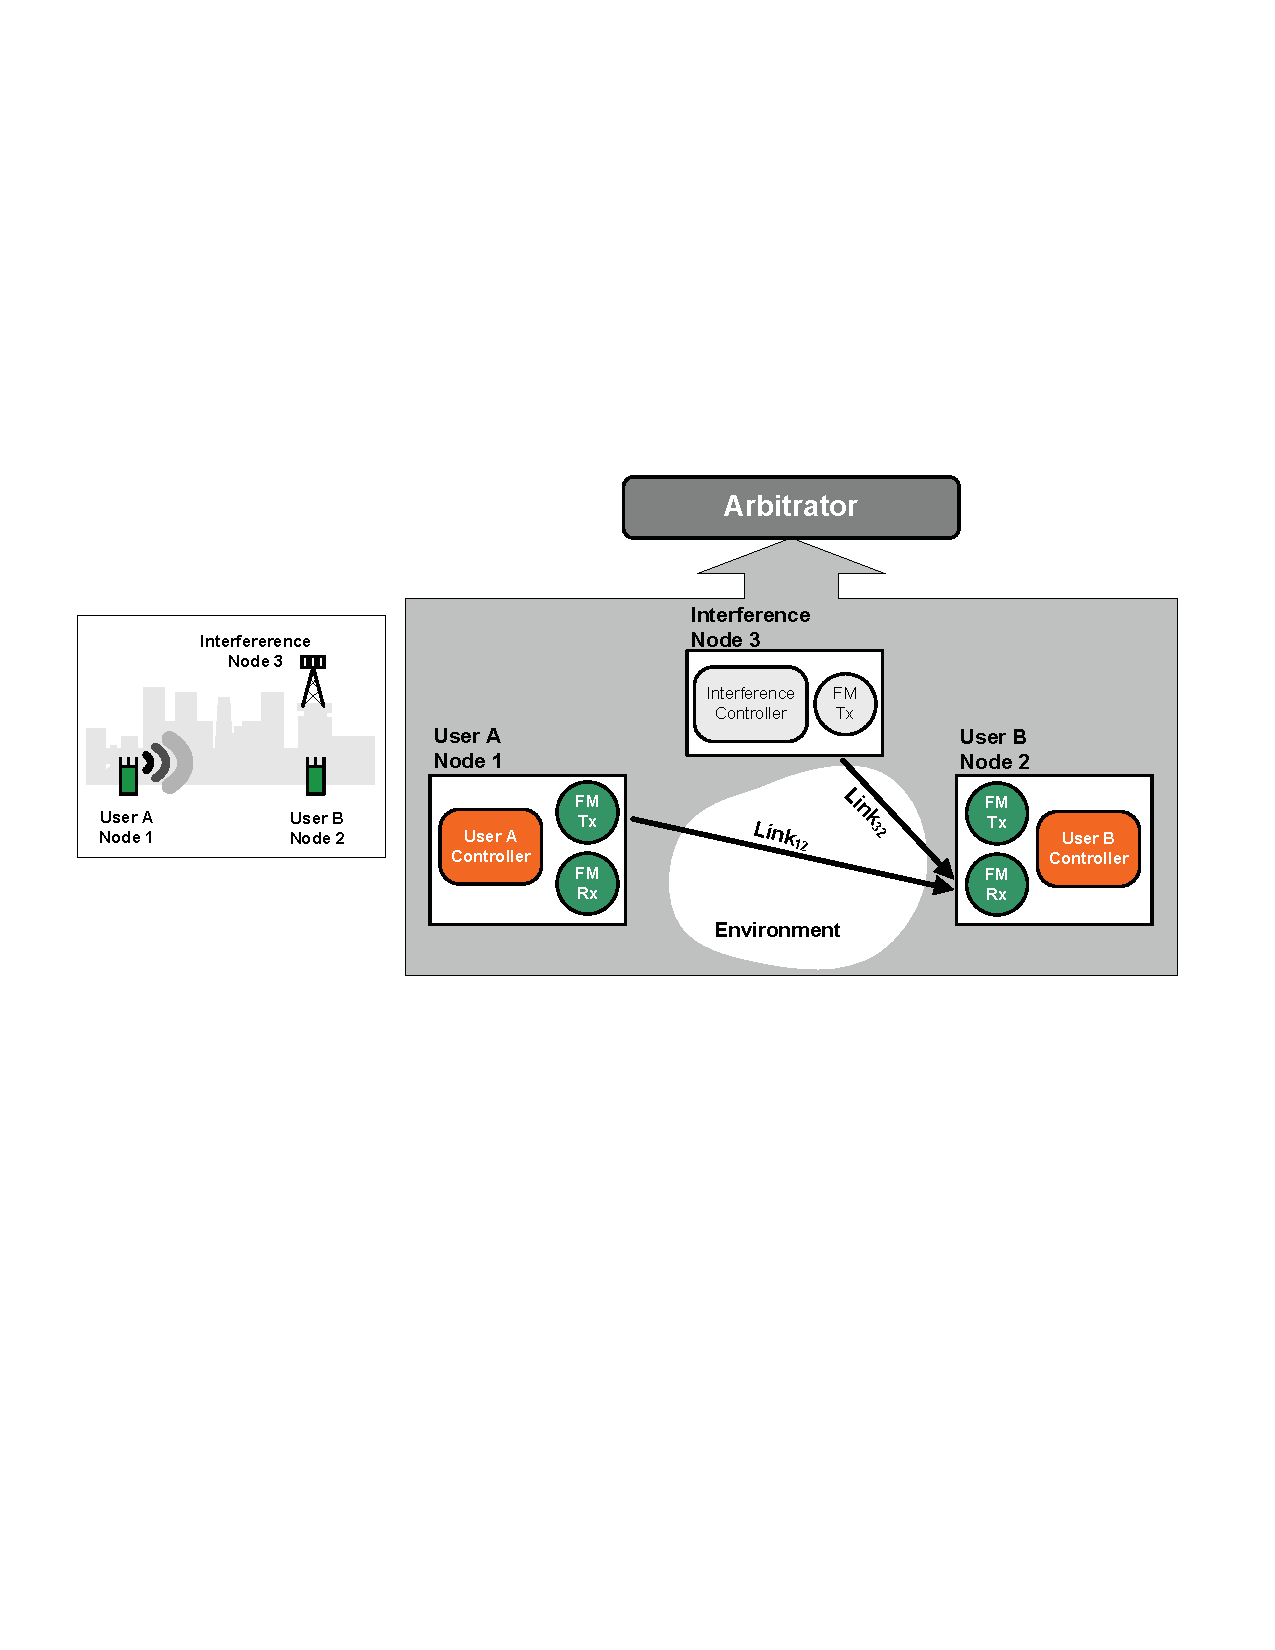
\includegraphics[width=6in]{figs/Software_Overview}
\caption{Example of how a scenario relates to software structure}
\label{fig:softwareOverview}
\end{figure}

The controller functions are state machines written in a specific
way so that they can coordinate with the LLAMAComm arbitrator.  The
coordination is handled through a request/acknowledge system.  Nodes
that wish to transmit or receive a segment of analog signal must
send a request to the arbitrator containing the segment start time
and segment duration.  The arbitrator coordinates execution order so
that any possible interference is included in a segment of received
signal.  In practice, this coordination is transparent to the user.

The remaining portions of the simulation---including the environment
and link objects---are created by the simulator and operate in the
background.  Basically, the user is responsible for programming the
portions of Figure \ref{fig:softwareOverview} that are in color.
Since LLAMAComm includes some pre-made interference sources, this
example would require the user to write only four MATLAB functions:
the FM transmit module, FM receive module, User A controller, and
User B controller.

This is a simple example, intended as a quick overview.  A more
complicated scenario would contain more nodes, and each node may
contain more than two modules.  There are also other features of the
simulator not yet mentioned, such as the special ``genie'' link.
These details, and more, are covered in the following chapters.

%
% This material is based upon work supported by the Defense Advanced Research
% Projects Agency under Air Force Contract No. FA8702-15-D-0001. Any opinions,
% findings, conclusions or recommendations expressed in this material are those
% of the author(s) and do not necessarily reflect the views of the Defense
% Advanced Research Projects Agency.
%
% © 2019 Massachusetts Institute of Technology.
%
%
% This program is free software; you can redistribute it and/or modify
% it under the terms of the GNU General Public License version 2 as
% published by the Free Software Foundation;
%
% THIS SOFTWARE IS PROVIDED BY THE COPYRIGHT HOLDERS AND CONTRIBUTORS "AS IS"
% AND ANY EXPRESS OR IMPLIED WARRANTIES, INCLUDING, BUT NOT LIMITED TO, THE
% IMPLIED WARRANTIES OF MERCHANTABILITY AND FITNESS FOR A PARTICULAR PURPOSE
% ARE DISCLAIMED. IN NO EVENT SHALL THE COPYRIGHT OWNER OR CONTRIBUTORS BE
% LIABLE FOR ANY DIRECT, INDIRECT, INCIDENTAL, SPECIAL, EXEMPLARY, OR
% CONSEQUENTIAL DAMAGES (INCLUDING, BUT NOT LIMITED TO, PROCUREMENT OF
% SUBSTITUTE GOODS OR SERVICES; LOSS OF USE, DATA, OR PROFITS; OR BUSINESS
% INTERRUPTION) HOWEVER CAUSED AND ON ANY THEORY OF LIABILITY, WHETHER IN
% CONTRACT, STRICT LIABILITY, OR TORT (INCLUDING NEGLIGENCE OR OTHERWISE)
% ARISING IN ANY WAY OUT OF THE USE OF THIS SOFTWARE, EVEN IF ADVISED OF THE
% POSSIBILITY OF SUCH DAMAGE.

\chapter{Tutorial} \label{chp:tutorial}

The purpose of this chapter is to demonstrate how to use LLAMAComm
through the study of one canonical example.  This chapter will first
walk through running the example which is provided with the
installation archive.  It will then delve into the the MATLAB code
used to implement the example radios.  By the end of this chapter,
the reader should be comfortable with the idea of simulating a new
radio in LLAMAComm.

\section{Installing LLAMAComm}

LLAMAComm is provided as a single archive file with the extension
\verb+.tar.gz+.  To install LLAMAComm, simply place the archive file
into a working directory.  If using UNIX or one of its variants,
unpack the archive using the command: \verb+tar -xzvf llamacommVxxx.tar.gz+
(where \verb+xxx+ depends on the version of
the software).  PC users can unpack the archive using WinZip.
Successfully unpacking the archive will create the following
directory structure:

\begin{verbatim}
     llamacomm/
         docs/
         simulator/
         user_code/
             examples/
                  BPSKNodes/
                  InterferenceNodes/
                  MIMONodes/
\end{verbatim}
%             InitGlobals.m
%             SetupPaths.m
%             StartExample.m

The directory \verb+docs/+ contains LLAMAComm documentation (this
file), \verb+simulator/+ contains the MATLAB code that implements
LLAMAComm, and \verb+user_code/+ contains user-defined radios.  The
installation archive ships with several examples in \verb+user_code/examples/+.

When developing radios for simulation in LLAMAComm, user code should
be confined to a folder within \verb+user_code/+. (e.g.
\verb+user_code/newradio/+).  
%The only exception is the startup script
%which must be located in \verb+llamacomm/+.  
Code within
\verb+simulator/+ should never be modified.

\section{Running the Example}

LLAMAComm is set up by default to run the example simulation.  Start
MATLAB and change the working directory to
\verb+installdir/llamacomm/user_code+. Run \verb+StartExample.m+. The example
simulation should finish without error in about 30 seconds.

\begin{figure}[h]
\centering
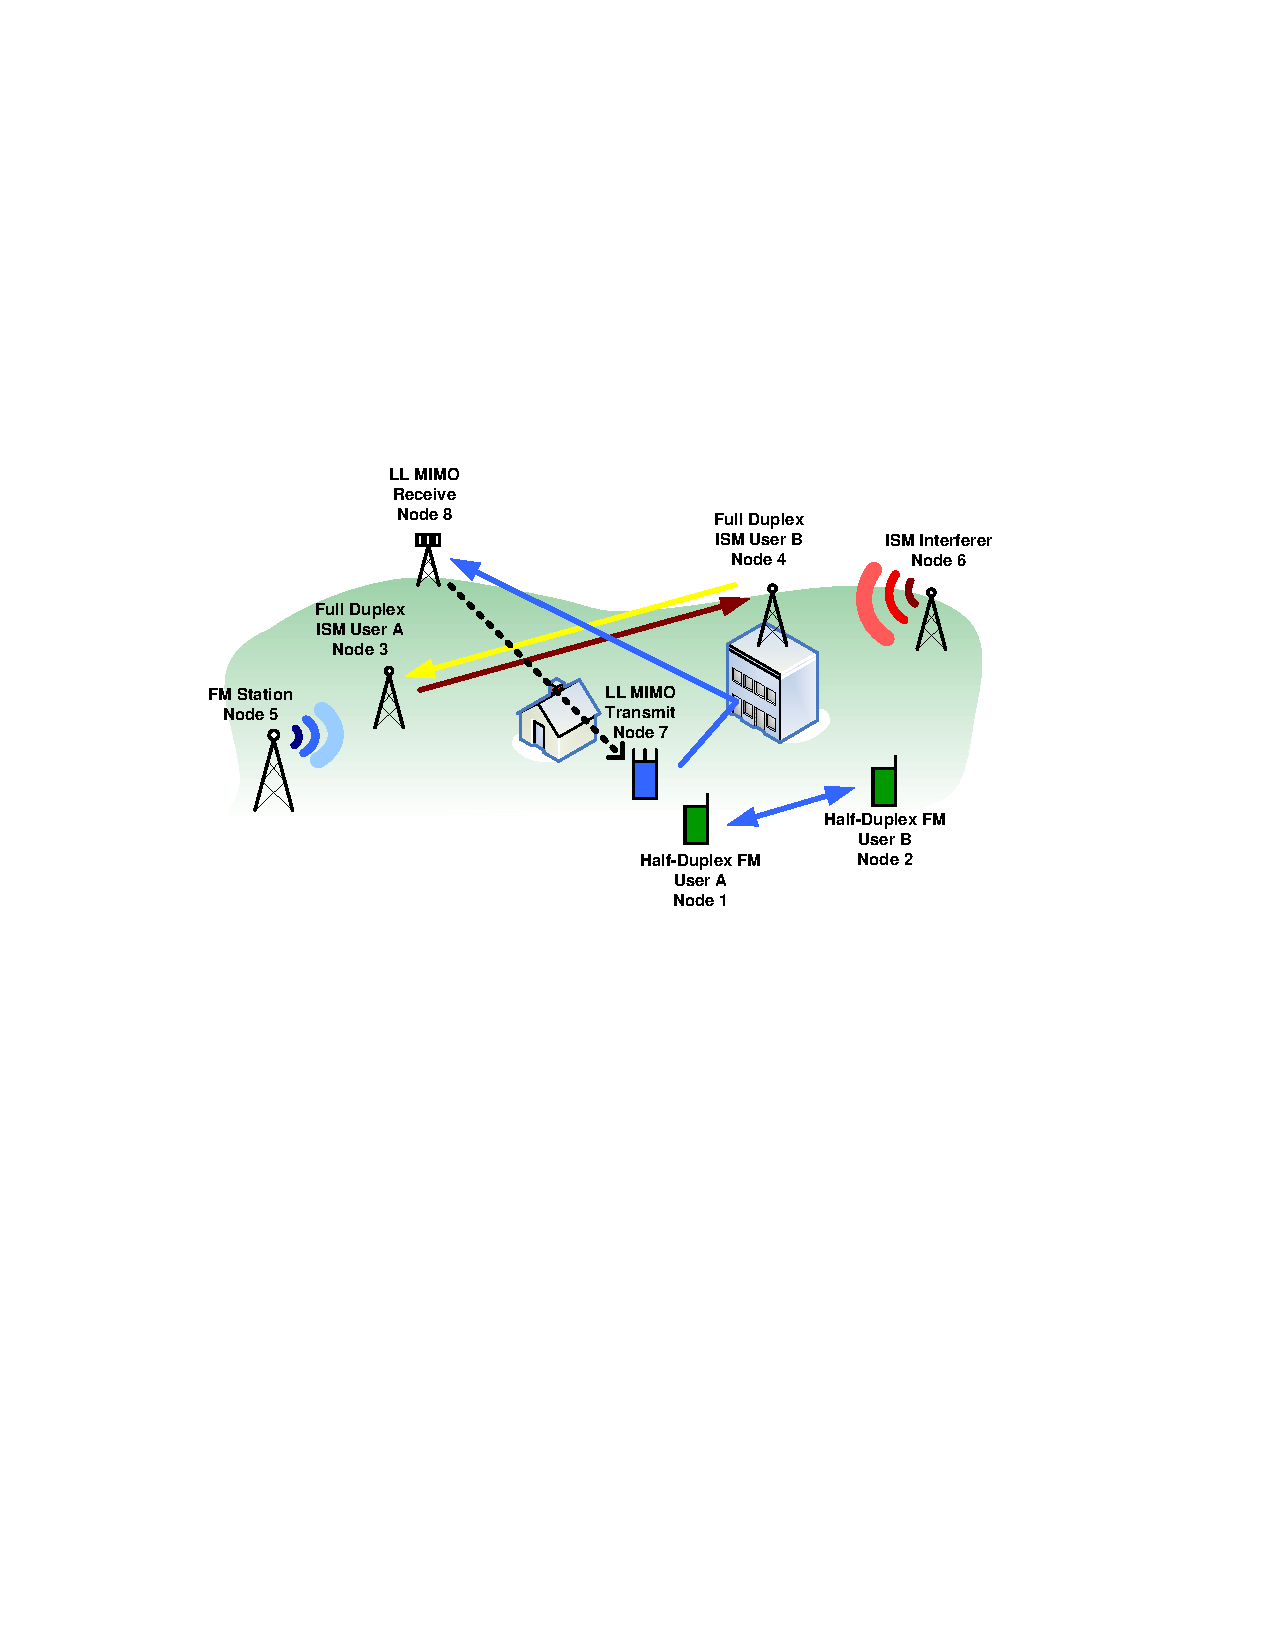
\includegraphics[width=6in]{figs/Canonical_Scenario}
\caption{The canonical example scenario}
\label{fig:canonicalEx}
\end{figure}

Figure \ref{fig:canonicalEx} shows a cartoon of the example
scenario. The example is a rural environment containing eight nodes.
The color of the arrows corresponds to the frequency of the
transmissions.  The two half-duplex nodes transmit and receive at
the same frequency in the FM radio band.  The two full-duplex nodes
transmit in two different frequency bands.  The yellow arrow
corresponds to 1500 MHz, while the dark red arrow corresponds to
2495 MHz (ISM band). Two interferers are present---one in the FM
band, and one in the ISM band. The LL MIMO transmitter transmits in
the FM band, but uses a special ``genie'' channel to send channel
information from the receiver back to the transmitter.  This genie
channel is represented by a black dotted line.  Note that genie transmit modules can ``multi-cast'' to multiple genie receive modules.

\subsection{Node Map}

LLAMAComm produces a couple plots by default.  When the example
scenario is run, a map is produced to show the positions and
relative heights of the nodes present in the scenario.
Figure~\ref{fig:nodeMap}(a) is a screen capture of the node map. The
map may be rotated and zoomed using the MATLAB figure toolbar.
Clicking with the regular mouse cursor\footnote{If nothing happens
when clicking, check that no buttons (including the arrow) are
depressed on the figure toolbar and try again.} on any of the node
names will produce a pop-up plot of the antenna positions and look
angles. Figure~\ref{fig:nodeMap}(b) shows this detail plot for the
node named \verb+AN+.

\begin{figure}[h]
\centering \mbox{
    \subfigure[Node map]{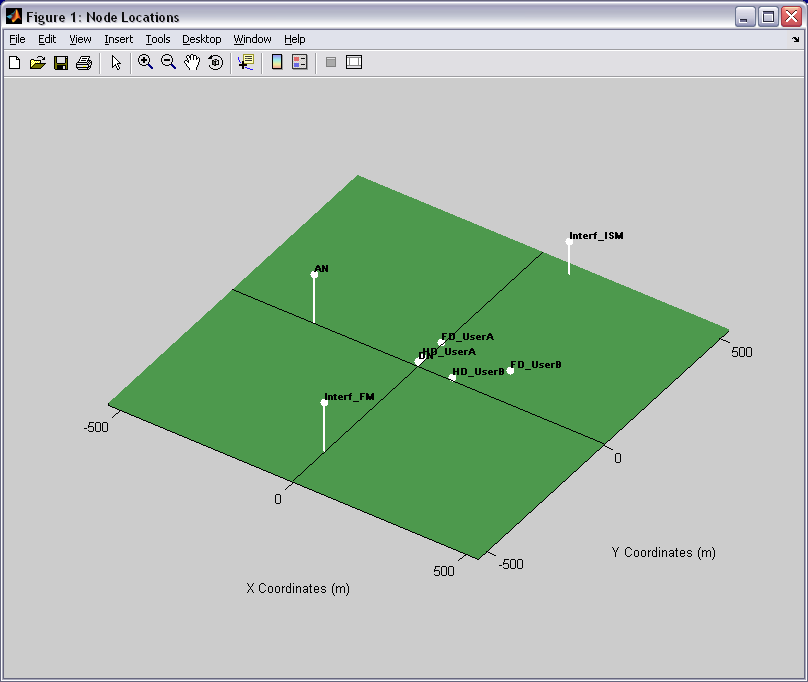
\includegraphics[width=3in]{figs/Node_Map}} \quad
    \subfigure[Antenna map]{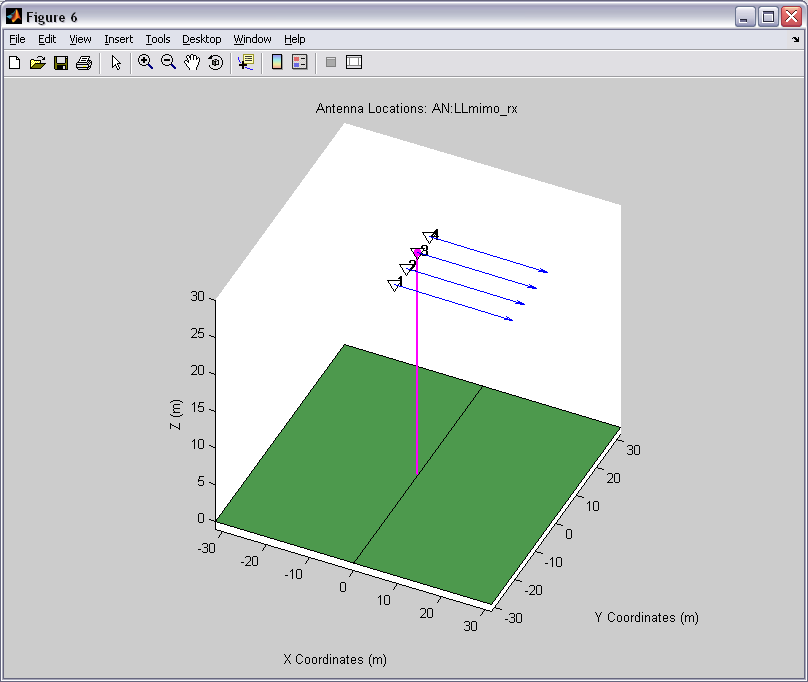
\includegraphics[width=3in]{figs/Antenna_Map}}
} \caption{Node map and detail plot of antenna positions}
\label{fig:nodeMap}
\end{figure}


\subsection{Timing Diagram Figure}\label{sec:tdSec}

Signal processing in the simulation is done in a block-wise fashion.
These blocks (which we refer to as segments) are drawn in a timing
diagram figure as the simulation runs.  Figure
\ref{fig:exTimingDiagram} shows a screen capture of the timing
diagram.

\begin{figure}[h]
\centering
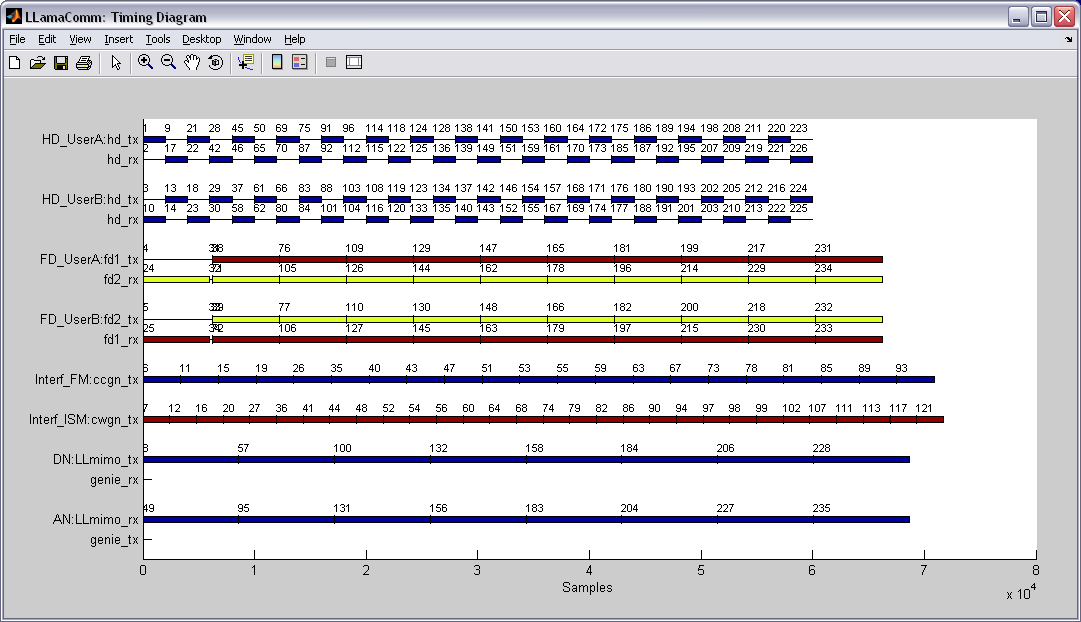
\includegraphics[width=6in]{figs/Example_Timing_Diagram}
\caption{Screen capture of timing diagram from example simulation}
\label{fig:exTimingDiagram}
\end{figure}

Each horizontal line in the diagram is associated with a module
within a node.  For example, the half-duplex radio (labeled
\verb+HD_UserA+) contains two modules: \verb+hd_tx+ and
\verb+hd_rx+. \verb+hd_tx+ is the BPSK transmit module, and
\verb+hd_rx+ is the BPSK receive module. This node alternates
between transmitting and receiving because it is operating in
half-duplex mode.  All the segments are blue because the radios are
operating at the same center frequency. In contrast, the full-duplex
nodes have a red segments and yellow segments because the modules
operate at different frequencies.

The small number near each segment indicates the order in which the
segment was processed.  This is mainly for debugging purposes, but
it is useful to note that the segments are not processed
sequentially.  Segments are processed out of order so that a receive
segment contains the contribution of all in-band signals present in
its duration.  This scheduling is handled by the simulator.

%Previous users of the Cogcom should also note that the LL MIMO nodes
%are named DN and AN.  This was done to show how Cogcom code can be
%ported to LLAMAComm.  The AN and DN become separate nodes, and the
%magic feedback loop is modeled by including special genie modules
%(more on this later).

After the simulation has finished running, clicking on any of the
rectangles in the timing diagram with the mouse cursor will bring up
a plot of the data in that segment.  It also is possible to define a
custom plot.  Figure \ref{fig:tdCallback} shows a picture of the
default plot and a custom plot.  Both plots show the power spectral
density in the right subplot.  In the left subplot, the default plot
shows the real (blue) and imaginary (green) parts of the ``analog''
waveform. The highlighted portion is the segment that was selected.
The adjacent segment is also plotted, but in thinner blue and green
lines, so that the continuity of the signal can be examined.  The
left subplot of the custom plot shows a constellation plot of the
beamformer output for the LL MIMO receiver.

\begin{figure}[h]
\centering \mbox{
    \subfigure[Default plot]{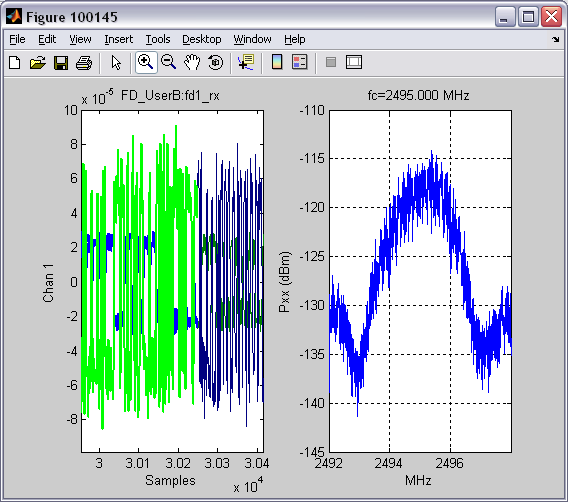
\includegraphics[width=3in]{figs/TD_Default_Callback}} \quad
    \subfigure[Custom plot]{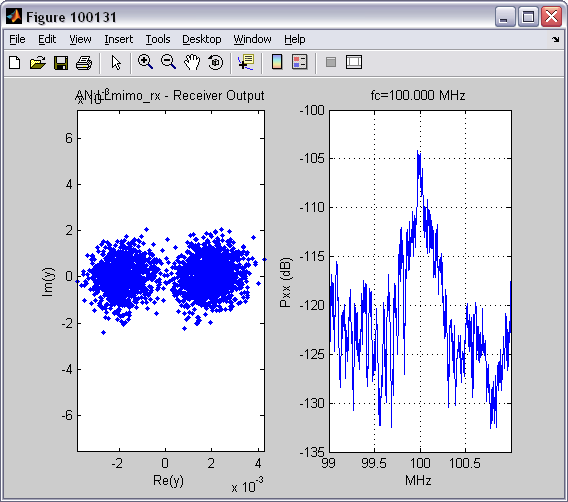
\includegraphics[width=3in]{figs/TD_Custom_Callback}} \quad
    }
\caption{Default plot for full-duplex UserB node and custom plot for
LL MIMO receive node} \label{fig:tdCallback}
\end{figure}

By clicking on other segments in the timing diagram, it should be
possible to observe the interaction between the various nodes.  For
example, segments of signal for \verb+FD_UserA:fd2_rx+ appear very
clean because they contain no interference.  In contrast, receive
segments for \verb+HD_UserA:hd_rx+ and \verb+HD_UserB:hd_rx+ are
very noisy because they contain interference from
\verb+Interf_FM:ccgn_tx+ and \verb+DN:LLmimo_tx+.

\subsection{Text Output}

The simulation also produces a great deal of text output.  Like
typical MATLAB programs, any function may write to the command
window.  The output from running the example simulation is shown
below. The LL MIMO transmitter and receiver dump many of their
operating parameters to screen as the simulation runs.  The
calculated bit error rates are also displayed at the end.  As
expected, links with interferers present exhibit a higher bit error
rate.

\begin{lstlisting}[name=output,numbers=none]
 ...
LLMimo Transmit Block 7/8
  txPower: 0.006163
LLMimo Receive Block 7/8
 rxDemod: eig(rNoise) (dB) = -36.6221 -54.2714  -74.452...
 rxDemod: frob(hEst)^2 (dB) = 1.7569
 rxDemod: eig(hhd) (dB) =2.29083 -12.2962 -26.7783 -29.1565
 Passed back to Tx:
         vTx: [0.3667+i*0.1181;0.2149+i*0.1234;0.2007+i*...
    domAtten: 1.6947
Simulation finished successfully.
HD_UserA->HD_UserB BER: 0.001133
HD_UserB->HD_UserA BER: 0.003533
FD_UserA->FD_UserB BER: 0.000300
FD_UserB->FD_UserA BER: 0.000000
LL MIMO example, DN->AN BER:0.010254
Elapsed time is 25.098511 seconds.
>>
\end{lstlisting}

\subsection{Simulator Output Files} \label{sec:simOutputFiles}

LLAMAComm produces a number of output files which can be used later
for analyzing the results.  These files include records of all
transmitted/received signals, transmitted/received bits, the timing
diagram figure, and workspace-level variables (including all
objects).  By default, the save directory is
\verb+llamacom/user_code/save/timestamp+, where \verb+timestamp+ is generated
based on the clock.  Each run of the simulation will produce a new
folder in the \verb+save/+ subdirectory with a different timestamp.

\begin{figure}[h]
\centering
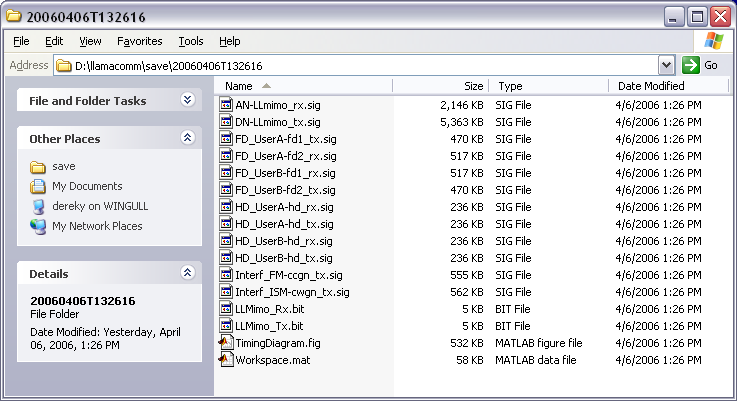
\includegraphics[width=5in]{figs/Save_Files}
\caption{Simulator output files}
\label{fig:saveFiles}
\end{figure}

Figure \ref{fig:saveFiles} shows the output produced by running the
example scenario.  These files are located in
\verb+llamacomm/user_code/save/20060406T132616+ because the simulation was
started at 1:26:16 pm on April 6, 2006.

Files with the extension \verb+.sig+ are saved automatically by
LLAMAComm. These files contain baseband samples of the
transmitted/received waveforms at the simulator's universal sample
rate.  There is one \verb+.sig+ file for each module in the
scenario. The naming convention is \verb+nodename-modulename.sig+.

Files with the \verb+.bit+ extension keep a record of the binary
bits transmitted or received.  These files are used to calculate the
bit error rate at the end of the simulation.  For short simulations,
transmitted and received bits can simply be stored within the node
objects.  For long simulations, however, it is more memory-efficient
to save this information to disk.  The half-duplex and full-duplex
examples in the following sections save the bits within the node
object, while the LL MIMO example writes the bits to disk.

\verb+TimingDiagram.fig+ is a saved copy of the timing diagram
discussed in \S\ref{sec:tdSec}.  Opening the saved figure in MATLAB
will bring back the figure window.  Callback plots (the plots that
appear when the segment rectangles are clicked with the mouse) will
function just as before since the data used to generate the plots is
stored in the \verb+.sig+ files.\footnote{The MATLAB paths may need
to be manually configured for the callbacks to work correctly.}

\verb+Workspace.mat+ contains all the variables accessible from the
MATLAB workspace at the completion of a simulation.  This includes a
copy of all the objects and setup properties.  From this
information, it is possible to determine all the properties of the
finished simulation.

\section{Creating Nodes, Modules, and Environments}
\label{sec:exampleSection}

The previous section explored the output generated by the example
simulation.  This section discusses the MATLAB code required to
actually implement the example.

LLAMAComm is implemented using MATLAB classes.  Instances of a class
are known as objects.  MATLAB classes are defined by creating a
subdirectory with the class name appended to the \verb+@+ character.
All functions within these class directories have access to object
variables---these are referred to as class methods.  Functions
outside the class directories normally do not have access to object
variables.\footnote{Please refer to the MATLAB documentation on
programming with classes for more detail.}

By using classes, information can be protected from improper sharing
or modification.  For example, a receiver should not know the true
channel matrix, so the channel matrix is hidden within a link object
where it cannot be directly accessed by code written for the
receiver.  For debugging, utilities have been included to display
the information to screen.

Using LLAMAComm requires some understanding of the various classes.
There are four classes used to implement the simulator:
\verb+@node+, \verb+@module+, \verb+@link+, and \verb+@environment+.
Users interested in simulating their own designs will need to become
familiar with the node and module classes. The environment and link
classes are not as important to the user.  The environment class is
used only once during startup by the user, and the link class is
accessed only by internal code.

Because of the divisions enforced by the simulator, the operation of
one set of radios does not affect another (other than possibly
causing interference, as it would in the real world).  As a result,
radio pairs can be designed independently.  Each example radio in
the simulation will be discussed separately in the following
sections. We will examine the MATLAB code closely.

\subsection{The Half-Duplex Radios} \label{sec:hdExample}

The half-duplex radios were the first example created for LLAMAComm.
They consist of two nearly identical transceivers that transmit a
very simple BPSK signal in the FM frequency band.  It is assumed
that the radios are already synchronized.

Nodes represent physical radios.  Since there are two radios in the
example scenario, there are two node objects.  Figure
\ref{fig:hdNodes} shows two nodes labeled \verb+HD_UserA+ and
\verb+HD_UserB+.  Conceptually, modules represent the physical layer
of a communication system, and controllers represent the link layer
as well as any operator actions.  Modules are responsible for the
modulation/demodulation and coding/decoding of a signal.  The
controller determines when to transmit/receive and what to do with
the data.  The controller implements the functionality of the
microcontroller in a physical radio.

\begin{figure}[h]
\centering
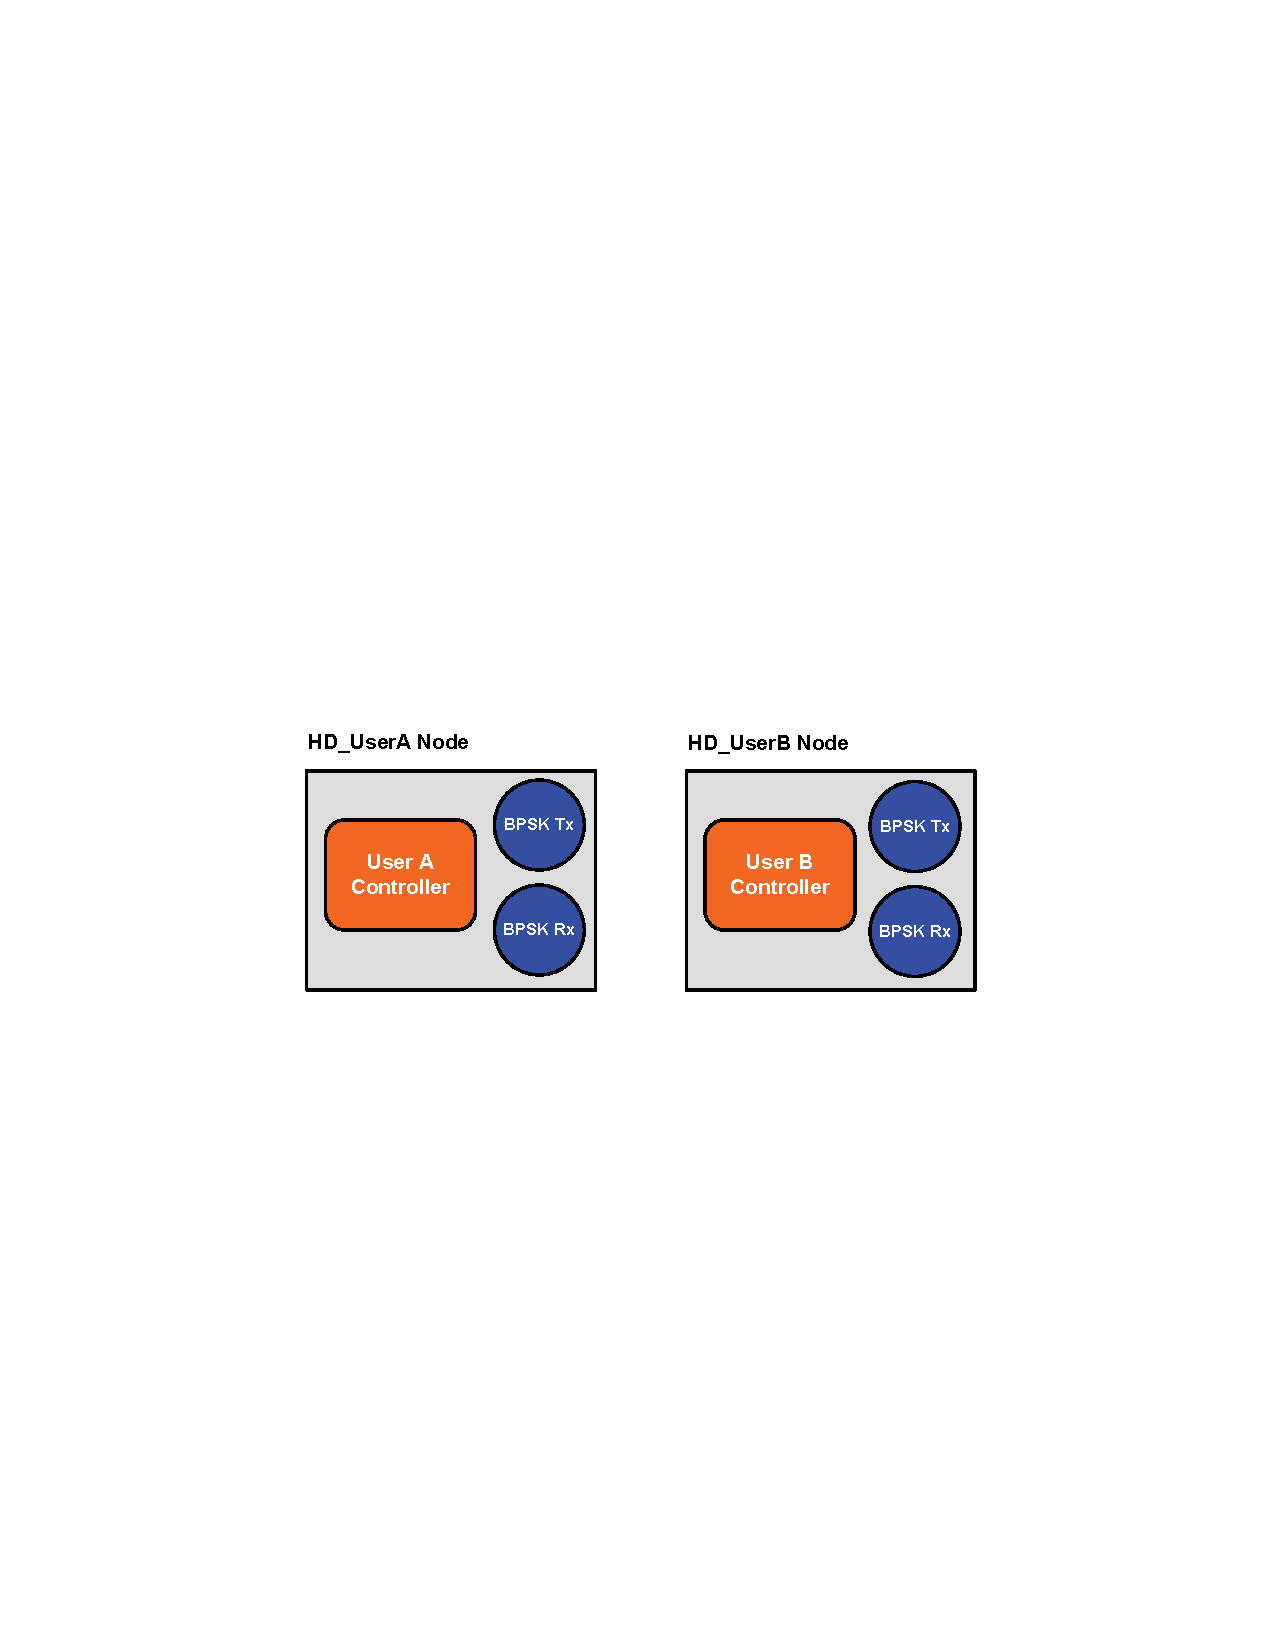
\includegraphics[width=3.5in]{figs/HD_Example}
\caption{Example half-duplex nodes} \label{fig:hdNodes}
\end{figure}

In LLAMAComm, modules must either be transmitters or receivers.  So,
for a transceiver, the minimum number of modules is two.  Note that
for certain communication systems, it may be desirable to have
multiple receive modules (a software radio, for example). This can
be simulated by adding any number of module objects into the node.
It is the controller's responsibility to decide which modules to use
at any given time for sending or receiving data.

Each node object in Figure \ref{fig:hdNodes} is shown to contain a
controller function and two module objects labeled \verb+BPSK Tx+
and \verb+BPSK Rx+.  The module objects are the same in the two
radios since they transmit in the same frequency using the same
transmission scheme. The two controller functions are very similar;
they are different only in that one controller starts in a transmit
state while the other starts in a receive state.

There are six files in the \verb+user_code/examples/BPSKNodes+ directory 
that are
used to implement the half-duplex radios: \verb+HD_BuildNodes.m+,
\verb+BPSK_Receive.m+, \verb+BPSK_Transmit.m+,
\verb+HD_UserA_Controller.m+, \verb+HD_UserB_Controller.m+,
\verb+HD_CalculateBER.m+.

\subsubsection{HD\_BuildNodes.m}

The basic steps for building any LLAMAComm node are shown below.  In
all the example radios provided, these steps are incorporated into a
``top-level'' function with the name \verb+*_BuildNodes.m+.

\begin{enumerate}
\item Specify required transmit and receive module properties
\item Provide handle to callback function that does the modulation/demodulation
\item Call module class constructor to create module objects
\item Specify required node properties
\item Provide handle to controller function
\item Include copies of the newly created module objects
\item Call node class constructor and return new node objects
\end{enumerate}

Code to construct the half-duplex nodes is found in
\verb+llamacomm/user_code/examples/BPSKNodes/HD_BuildNodes.m+.  
Let us walk through
the file.  The block of code listed below is the function header and
help comments. The build functions return an array of completed node
objects.

\begin{lstlisting}[name=hdBuildNodes]
function hdNodes = HD_BuildNodes

% Function HD_BuildNodes.m:
% Example function/script for building example half-duplex nodes with
% common transmit/receive modules and user parameters.
%
% USAGE: hdNodes = BuildUserNodes
%
% Input arguments:
%  -none-
%
% Output arguments:
%  hdNodes  (1xN Node obj array) Newly-created user nodes
%
\end{lstlisting}

The next block of code defines two structs that contain all the
required properties for building a module. \verb+hd_tx_mod_params+
defines the transmit module and \verb+hd_rx_mod_params+ defines the
receive module.\footnote{Future versions of this code may have
default values assigned for some variables such as wall material and
antenna type.}

\begin{lstlisting}[firstnumber = 22, name=hdBuildNodes]
% Define transmit/recieve modules

hd_tx_mod_params.name = 'hd_tx';
hd_tx_mod_params.callbackFcn = @BPSK_Transmit;
hd_tx_mod_params.fc = 98.5e6;
hd_tx_mod_params.type = 'transmitter';
hd_tx_mod_params.loError = 0;
hd_tx_mod_params.antType = {'dipole_halfWavelength'};
hd_tx_mod_params.antPosition = [0 0 0];
hd_tx_mod_params.antPolarization = {'v'};
hd_tx_mod_params.antAzimuth = [0];
hd_tx_mod_params.antElevation = [0];
hd_tx_mod_params.exteriorWallMaterial = 'none';
hd_tx_mod_params.distToExteriorWall = [0];
hd_tx_mod_params.exteriorBldgAngle = [0];
hd_tx_mod_params.numInteriorWalls = [0];

hd_rx_mod_params.name = 'hd_rx';
hd_rx_mod_params.callbackFcn = @BPSK_Receive;
hd_rx_mod_params.fc = 98.5e6;
hd_rx_mod_params.type = 'receiver';
hd_rx_mod_params.loError = 0;
hd_rx_mod_params.antType = {'dipole_halfWavelength'};
hd_rx_mod_params.antPosition = [0 0 0];
hd_rx_mod_params.antPolarization = {'v'};
hd_rx_mod_params.antAzimuth = [0];
hd_rx_mod_params.antElevation = [0];
hd_rx_mod_params.exteriorWallMaterial = 'none';
hd_rx_mod_params.distToExteriorWall = [0];
hd_rx_mod_params.exteriorBldgAngle = [0];
hd_rx_mod_params.numInteriorWalls = [0];
hd_rx_mod_params.noiseFigure = 6; % (dB) noise figure of receiver

hd_tx_mod = module(hd_tx_mod_params);
hd_rx_mod = module(hd_rx_mod_params);


\end{lstlisting}

Module names (\verb+hd_tx+ and \verb+hd_rx+, in this example) must
be unique for a given node.  \verb+callbackFcn+ is the function
handle to the function that performs the modulation/demodulation. In
this case, the functions are \verb+BPSK_Receive.m+ and
\verb+BPSK_Transmit.m+. MATLAB syntax uses the \verb+@+ symbol to
turn a function name into a function handle. \verb+fc+ specifies the
center frequency of the modulated signal. \verb+type+, is a string
that tells LLAMAComm whether the module is a transmitter or a
receiver. Details on the other properties can be found in the
reference section of the documentation.

The last two lines of the block of code shown above (lines 55-56)
are calls to the module class constructor.  The constructor expects
a struct with the specific field names provided in the example.  It
returns a module object.  In this example, two modules are produced:
\verb+hd_tx_mod+ and \verb+hd_rx_mod+.

\begin{lstlisting}[name=hdBuildNodes]
% Define nodes

userA_node_params.name = 'HD_UserA';
userA_node_params.location = [0 20 3];
userA_node_params.velocity = [0 0 0];
userA_node_params.controllerFcn = @HD_UserA_Controller;
userA_node_params.modules = [hd_tx_mod hd_rx_mod];

userB_node_params.name = 'HD_UserB';
userB_node_params.location = [100 0 2];
userB_node_params.velocity = [0 0 0];
userB_node_params.controllerFcn = @HD_UserB_Controller;
userB_node_params.modules = [hd_tx_mod hd_rx_mod];

userA_node = node(userA_node_params);
userB_node = node(userB_node_params);


\end{lstlisting}

The code block above creates two node objects.  It is similar in
structure to the code used to create the module objects. The first
parts assigns properties in a struct.  The last two lines call the
node class constructor.

The node name must be unique within a scenario.  The node location
is specified in rectangular coordinates in meters.  The node
velocity is in meters/second.  The property \verb+controllerFcn+ is
a function handle. In this case, node \verb+HD_UserA+ is using the
controller function defined by \verb+HD_UserA_Controller.m+.

The \verb+modules+ property should be an array of module objects.
This example uses the two modules defined earlier in the build
function: \verb+hd_tx_mod+ and \verb+hd_rx_mod+.

The next block of code in the file sets user-defined parameters in
the node objects.

\begin{lstlisting}[name=hdBuildNodes]
% Set user parameters

userParams.power = 10; % (Watts)
userParams.dataLen = 800;
userParams.trainingLen = 200;
userParams.nOversamp = 2;
userParams.bitLen = userParams.dataLen+userParams.trainingLen;
userParams.blockLen = userParams.nOversamp*userParams.bitLen;

userParams.trainingSeq = rand(1,userParams.trainingLen)>.5;

userParams.nBlocksToSim = 15;
userParams.receivedBlocks = 0;
userParams.transmittedBlocks = 0;

userParams.txBits = zeros(userParams.nBlocksToSim,...
                          userParams.bitLen,'uint8');
userParams.rxBits = zeros(userParams.nBlocksToSim,...
                          userParams.bitLen,'uint8');

userParams.equalizerLen = 21;
userParams.equalizerDelay = 10;

userA_node = SetUserParams(userA_node,userParams);
userB_node = SetUserParams(userB_node,userParams);


\end{lstlisting}

User parameters are a special part of the node.  These parameters,
which consist of anything that can be put into a single MATLAB
structure, can be written and read at the user's discretion.  This
area is useful for storing information that a physical radio would
have in its EEPROM, such as a training sequence, packet length, or
initial transmit power.  The user parameters are also useful for
passing information between the controller function and the
transmit/receive functions.  In fact, \emph{this is the only method
of communication between the modules and the controller function}.

The user parameters are stored within a node, so they are accessed
using class methods:  \verb+SetUserParams()+ and
\verb+GetUserParams()+. This example sets the power, defines the
data block structure, and sets aside memory to hold transmitted and
received bits.  (This works since this is a small example.  Larger
examples such as LL MIMO store the bits to file.)  The last two
lines call \verb+SetUserParams()+ to store the structure into the
node object.

\begin{lstlisting}[name=hdBuildNodes]
% Put user nodes into array
hdNodes = [userA_node userB_node];
\end{lstlisting}

Finally, the last line of the function returns the two newly created
half-duplex nodes in a 1x2 array.

\subsubsection{BPSK\_Transmit.m and BPSK\_Receive.m}

As mentioned in the previous sections, \verb+BPSK_Transmit.m+ and
\verb+BPSK_Receive.m+ define the physical layer of the example
half-duplex radios.  Code from \verb+BPSK_Transmit.m+ is listed
below.

\begin{lstlisting}[name=bpskTx]
function [nodeobj,sig] = BPSK_Transmit(nodeobj,modname,blockLen)

% Function BPSK_Transmit.m:
% This is an example of a user-written callback function for a module
% object.  It generates or loads data to transmit. The output signal 
% should be analog baseband, and can be multichannel.
%
% This example is a single-channel BPSK transmitter.  2x oversampled.
% There is no filtering or pulse shaping, so the signal is full bandwidth.
%
% USAGE: [nodeobj,sig] = BPSK_Transmit(nodeobj,modname,blockLen)
%
% Input arguments:
%  nodeobj    (node obj) Parent node object
%  modname    (string) The name of the module that has activated this
%              callback function
%  blockLen   (int) The block length of the analog signal expected
%              by the arbitrator
%
% Output arguments:
%  nodeobj    (node obj) Modified copy of the node object
%  sig        (NxblockLen) Analog baseband signal for N channels
%
% See also: BPSK_Receive.m
\end{lstlisting}

Transmit and receive callback functions must use these exact input
and output arguments.  This is required to properly interface to the
simulator's arbitrator function.  \verb+BPSK_Transmit()+ takes in a
node object, the module name, and the block length of the signal to
be transmitted.  It returns a modified node object (the user
properties will be modified) and a single segment of complex
baseband signal at the simulator's universal baseband sample rate.

The function starts by retrieving the user parameters.  User
parameters are stored in the node object and must be retrieved using
\verb+GetUserParams()+.  This is shown in the following block of
code.

\begin{lstlisting}[firstnumber=31, name=bpskTx]
% Load user parameters
p = GetUserParams(nodeobj);

\end{lstlisting}

In the example, data is randomly generated.  This is shown in the
code fragment below.  The code produces random $\pm 1$'s and
attaches the fixed training sequence.  The data is then duplicated
using \verb+repmat+ to give an effect data rate of \verb+fs/2+.
\verb+fs+ is the universal simulation sample rate set in
\verb+InitGlobals.m+. It is set by default to 12.5 MHz.

\begin{lstlisting}[name=bpskTx]
% Make some random data and attach training sequence
randdata = rand(1,p.dataLen)>.5;
bits = [p.trainingSeq randdata];
sig = -(bits*2-1);

% Upsample by duplicating bits
sig = repmat(sig,p.nOversamp,1);
sig = sig(:).';

\end{lstlisting}

It is also possible to read data from file or generate it in the
controller function and then pass the data block to the transmit
function.  In order keep the distinction between physical layer and
link layer as sharp as possible, it is preferable to build the data
block in the controller function if memory constraints allow.  This
is done in the LL MIMO example (\S\ref{sec:llmimoNodes}).

\begin{lstlisting}[name=bpskTx]
% Calculate signal power (Watts)
filePow = var(sig);

% Set the transmitted signal power
sig = sqrt(p.power/(filePow))*sig;

\end{lstlisting}

The power of the transmitted signal is adjusted.  The units of
\verb+sig+ are volts.  The units of power are watts.  Power is
calculated by assuming a 1$\Omega$ load.  This convention is
followed throughout the simulation.

\begin{lstlisting}[name=bpskTx]
% Check blockLen
if size(sig,2) ~= blockLen
    error('Block length of Tx data is wrong.');
end



\end{lstlisting}

The value of \verb+blockLen+ is set by the controller function.  It
is passed into the transmit function by the arbitrator.  This block
of code does a quick check to make sure that the final block length
of the transmit signal is correct.

\begin{lstlisting}[name=bpskTx]
% Save txbits
p.transmittedBlocks = p.transmittedBlocks+1;
p.txBits(p.transmittedBlocks,:) = bits;

% Save user params
nodeobj = SetUserParams(nodeobj,p);
\end{lstlisting}

Finally, \verb+SetUserParams()+ must be used to save the transmitted
bits into the user parameters.  The values are later used to
calculate the bit error rate.

\verb+BPSK_Receive.m+ is very similar to \verb+BPSK_Transmit.m+. The
difference is that it receives and demodulates the bits.  The code
for \verb+BPSK_Receive+ is included below for comparison.

\begin{lstlisting}[name=bpskRx]
function nodeobj = BPSK_Receive(nodeobj,modname,sig)

% Function BPSK_Receive.m:
% This is an example of a user-written callback function for a 
% receive module.  This example demodulates an analog, BPSK signal.
%
% This example is designed to work with BPSK_Transmit
%
% USAGE: nodeobj = BPSK_Receive(nodeobj,modname,sig)
%
% Input arguments:
%  nodeobj    (node obj) Parent node object
%  modname    (string) The name of the module that has activated this
%              callback function
%  sig        (NxblockLen) Analog baseband signal for N channels
%
% Output arguments:
%  nodeobj    (node obj) Modified copy of the node object
%
% See also: BPSK_Transmit.m

%%%%%%%%%%%%%%%%%%%%%%%%%%%%%%%%%%%%%%%%%%%%%%%%%%%%%%%%%%%%%%%%%
% Copyright (c) 2006-2016 Massachusetts Institute of Technology %
% All rights reserved.   See software license below.            %
%%%%%%%%%%%%%%%%%%%%%%%%%%%%%%%%%%%%%%%%%%%%%%%%%%%%%%%%%%%%%%%%%

% Load user parameters
p = GetUserParams(nodeobj);

% Downsample
sig = sig(1:p.nOversamp:end);

% Demod
nSamps = length(sig);
nTrain = p.trainingLen;
sTrain = -(p.trainingSeq*2- 1);

% adapt equalizer
eqLen = p.equalizerLen;
eqDelay = p.equalizerDelay;
R = toeplitz([sig(1) zeros(1,eqLen-1)], sig(1:nTrain));
Sd = [zeros(1,eqDelay),sTrain(1:nTrain-eqDelay)];
f = Sd*R'*inv(R*R');

% equalize and extract bit estimates 
nBits = p.bitLen;
sHat = conv(sig,f);
bits = real(sHat(eqDelay+1:nBits+eqDelay))<0;

% Save rx bits
p.receivedBlocks = p.receivedBlocks+1;
p.rxBits(p.receivedBlocks,:) = bits;

% Save user params
nodeobj = SetUserParams(nodeobj,p);
\end{lstlisting}

\subsubsection{HD\_UserA\_Controller.m and HD\_UserB\_Controller.m}

The structure for any controller function can be described as a
finite state machine.  All the examples were developed by first
drawing the state diagram.  Figure \ref{fig:hdState} shows the state
diagrams for the \verb+HD_UserA+ controller and the \verb+HD_UserB+
controller. The outputs are shown in blue, and the inputs are shown
in green.

\begin{figure}[h]
\centering
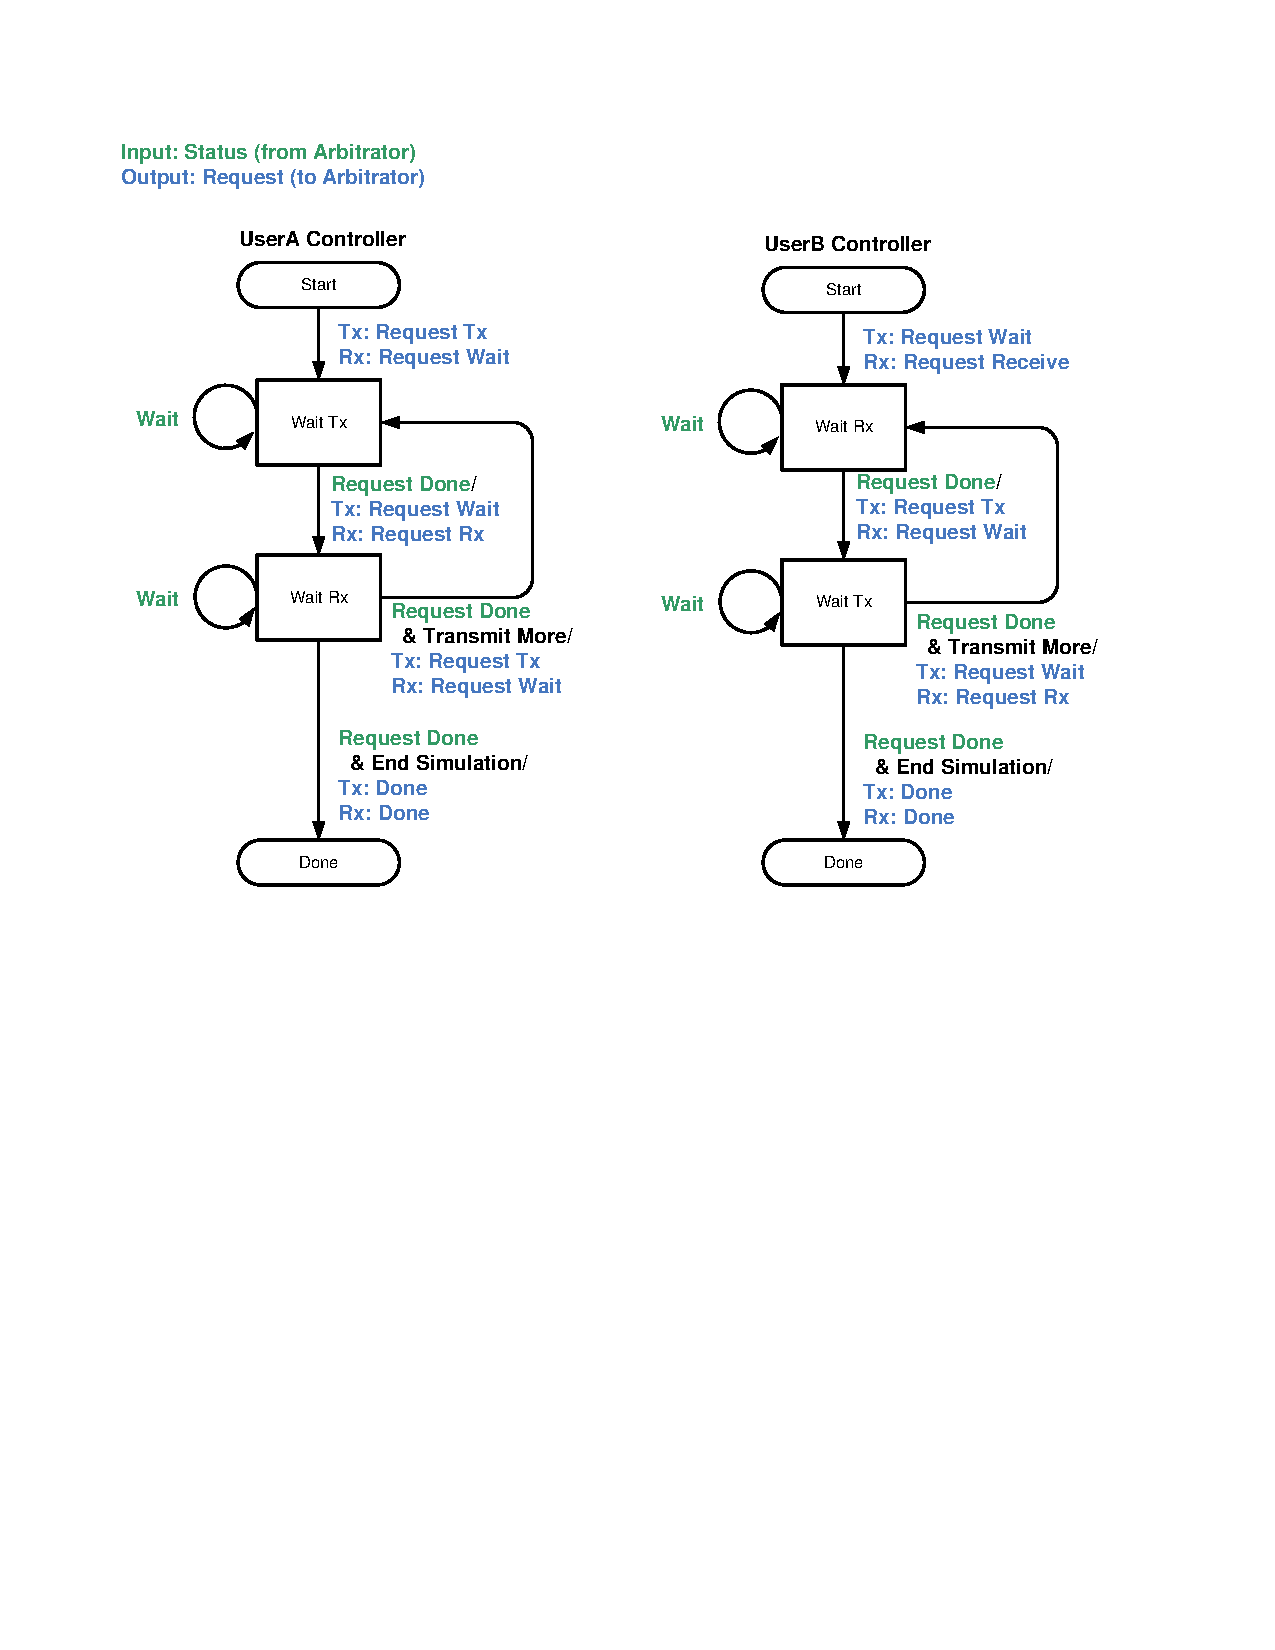
\includegraphics[width=5in]{figs/HD_State_Diagram}
\caption{State diagrams for half-duplex controller functions}
\label{fig:hdState}
\end{figure}

In order to transmit or receive, a request must be made to the
arbitrator.  During each iteration of the simulation loop, the
controller checks the status of the node's modules to see if the
requests are complete.  Once complete, the controller moves on to
the next state.  Otherwise, it continues to wait.  Note that it is
possible to write a controller so that the simulation stalls.  The
arbitrator is designed to detect such a state and abort the
simulation.  This will be discussed in more detail in
Section~\ref{sec:simExecution}.

Implementing the state machines shown in Figure \ref{fig:hdState} is
relatively straight-forward.  The code for
\verb+HD_UserA_Controller+ is examined in the listing below.

\begin{lstlisting}[name=hdState]
function [nodeobj,status] = HD_UserA_Controller(nodeobj)

% Function HD_UserA_Controller.m:
% Controller state machine for example Half-Duplex radio.  
% These controllers assume that the user nodes are already synchronized.  
% The UserA and UserB controllers are identical except that UserA starts 
% by sending a block and UserB starts by receiving a block.  
% The controller switches to the done state after receiving/sending a set 
% number of blocks.
%
% USAGE: [nodeobj,status] = HD_UserA_Controller(nodeobj)
%
% Input arguments:
%  nodeobj    (node obj) Parent node object.  
%
% Output arguments:
%  nodeobj    (node obj) Modified copy of node object
%  status     (string) Either 'running' or 'done'
%

%%%%%%%%%%%%%%%%%%%%%%%%%%%%%%%%%%%%%%%%%%%%%%%%%%%%%%%%%%%%%%%%%
% Copyright (c) 2006-2016 Massachusetts Institute of Technology %
% All rights reserved.   See software license below.            %
%%%%%%%%%%%%%%%%%%%%%%%%%%%%%%%%%%%%%%%%%%%%%%%%%%%%%%%%%%%%%%%%%

status = 'running';  % Default status

\end{lstlisting}

The function headers for all controller functions need to have the
same input and outputs.  The controller function takes in a node
object and returns a modified node object and a status string.  The
status string is used to detect when a simulation is finished.  On
line 26, the status is set to \verb+'running'+.  When the controller
reaches the \verb+done+ state, the status is set to \verb+'done'+
(line 76).

The user parameters and current state are stored within the node
object.  They are extracted using the functions
\verb+GetUserParams()+ and \verb+GetNodeState()+.  This is shown
below.

\begin{lstlisting}[name=hdState]
% Load user parameters
p = GetUserParams(nodeobj);

% Get current node state
currState = GetNodeState(nodeobj);

\end{lstlisting}

The next code block implements the state machine shown in Figure
\ref{fig:hdState}.  When a module needs to do something, it raises a
request flag that the simulation arbitrator sees.  Requests are set
using the function \verb+SetModuleRequest()+.  A request consists of
the node object, the module name, a job (\verb+wait+,
\verb+transmit+, \verb+receive+, or \verb+done+), and a block
length. The block length tells the arbitrator how many samples are
in the segment of signal to be processed.  The arbitrator uses this
information to determine the execution order of the simulation.

\begin{lstlisting}[name=hdState]
% State machine next-state and output "logic"
switch currState
    case 'start'
        % Set up module for transmission of 1 block
        nodeobj = SetModuleRequest(nodeobj,'hd_tx','transmit',p.blockLen);
        nodeobj = SetModuleRequest(nodeobj,'hd_rx','wait',p.blockLen);
        nextState = 'transmit_wait';
        
    case 'transmit_wait'
        requests = CheckRequestFlags(nodeobj);
        if requests==0
            % Transmission done, receive
            nodeobj = SetModuleRequest(nodeobj,'hd_tx','wait',p.blockLen);
            nodeobj = SetModuleRequest(nodeobj,'hd_rx','receive',p.blockLen);
            nextState = 'receive_wait';
        else
            % All requests not satisfied, wait
            nextState = 'transmit_wait';
        end

    case 'receive_wait'
        requests = CheckRequestFlags(nodeobj);
        if requests==0 
            if  p.receivedBlocks>=p.nBlocksToSim
                % Goto done
                nodeobj = SetModuleRequest(nodeobj,'hd_tx','done');
                nodeobj = SetModuleRequest(nodeobj,'hd_rx','done');
                nextState = 'done';
            else
                % Receive done, go back to transmit
                nodeobj = SetModuleRequest(nodeobj,'hd_tx','transmit',p.blockLen);
                nodeobj = SetModuleRequest(nodeobj,'hd_rx','wait',p.blockLen);
                nextState = 'transmit_wait';
            end
        else
            % Requests pending, wait
            nextState = 'receive_wait';
        end
        
    case 'done'
        % Done!
        nextState = 'done';
        status = 'done';
                
    otherwise
        error(sprintf('Unknown state: %s',currState));
end

\end{lstlisting}

As the simulation runs, the arbitrator lowers request flags that
have been satisfied.  \verb+CheckRequestFlags()+ checks to see if
requests for all modules within the node have been satisfied.

For every sample in the simulation, each module must be
transmitting, receiving, or waiting.  If this rule is not followed,
the simulation will stall.  The only exception is the \verb+done+
job. Once a module is marked as \verb+done+, it is ignored by the
arbitrator.

Finally, the state and the user parameters are stored using
\verb+SetNodeState()+ and \verb+SetUserParams()+ in the code block
listed below.  This saves the state and user parameters so that they
can be loaded the next time the controller function is run.

\begin{lstlisting}[name=hdState]
% Set next state
nodeobj = SetNodeState(nodeobj,nextState);

% Store possibly modified user params
nodeobj = SetUserParams(nodeobj,p);
\end{lstlisting}


\subsubsection{HD\_CalculateBER.m}

The bit error rate (BER) is a commonly calculated metric for
communication simulations.  The following function demonstrates how
to calculate the BER in a simple simulation where the sent and
received bits are stored within the user parameters.

\begin{lstlisting}[name=ber]
function ber = HD_CalculateBER(nodes)

% Function HD_CalculateBER.m:
% Calculates the Bit-Error Rate for each of the two user nodes.
%
% USAGE:  ber = HD_CalculateBER(nodes)
%
% Input arguments:
%  nodes     (node obj array, 1xN) Node objects
%
% Output arguments:
%  ber       (1x2) HD_UserA->HD_UserB and HD_UserB->HD_UserA BER
%

%%%%%%%%%%%%%%%%%%%%%%%%%%%%%%%%%%%%%%%%%%%%%%%%%%%%%%%%%%%%%%%%%
% Copyright (c) 2006-2016 Massachusetts Institute of Technology %
% All rights reserved.   See software license below.            %
%%%%%%%%%%%%%%%%%%%%%%%%%%%%%%%%%%%%%%%%%%%%%%%%%%%%%%%%%%%%%%%%%


% Extract user parameters
UA = GetUserParams(FindNode(nodes,'HD_UserA'));
UB = GetUserParams(FindNode(nodes,'HD_UserB'));

% Calculate BER
errAB = find(xor(UA.txBits,UB.rxBits));
errBA = find(xor(UB.txBits,UA.rxBits));

berAB = length(errAB)/prod(size(UA.txBits));
berBA = length(errBA)/prod(size(UB.txBits));

ber(1) = berAB;
ber(2) = berBA;

% Print results to screen
fprintf('HD_UserA->HD_UserB BER: %f\n',berAB);
fprintf('HD_UserB->HD_UserA BER: %f\n',berBA);
\end{lstlisting}

This function is designed to be run from the top level of the
simulation.  It has access to all nodes in the simulator.  The
relevant node is found using \verb+FindNode()+.  The transmitted and
received bits are extracted using \verb+GetUserParams()+.  The bits
are compared, and the results are printed to screen.

\subsection{The Full-Duplex Radios}

The full-duplex radio example is very similar to the half-duplex
example.  The difference is that the transmit and receive modules
operate at different frequencies, and the controller function
activates both transmit and receive modules simultaneously.

\begin{figure}[h]
\centering
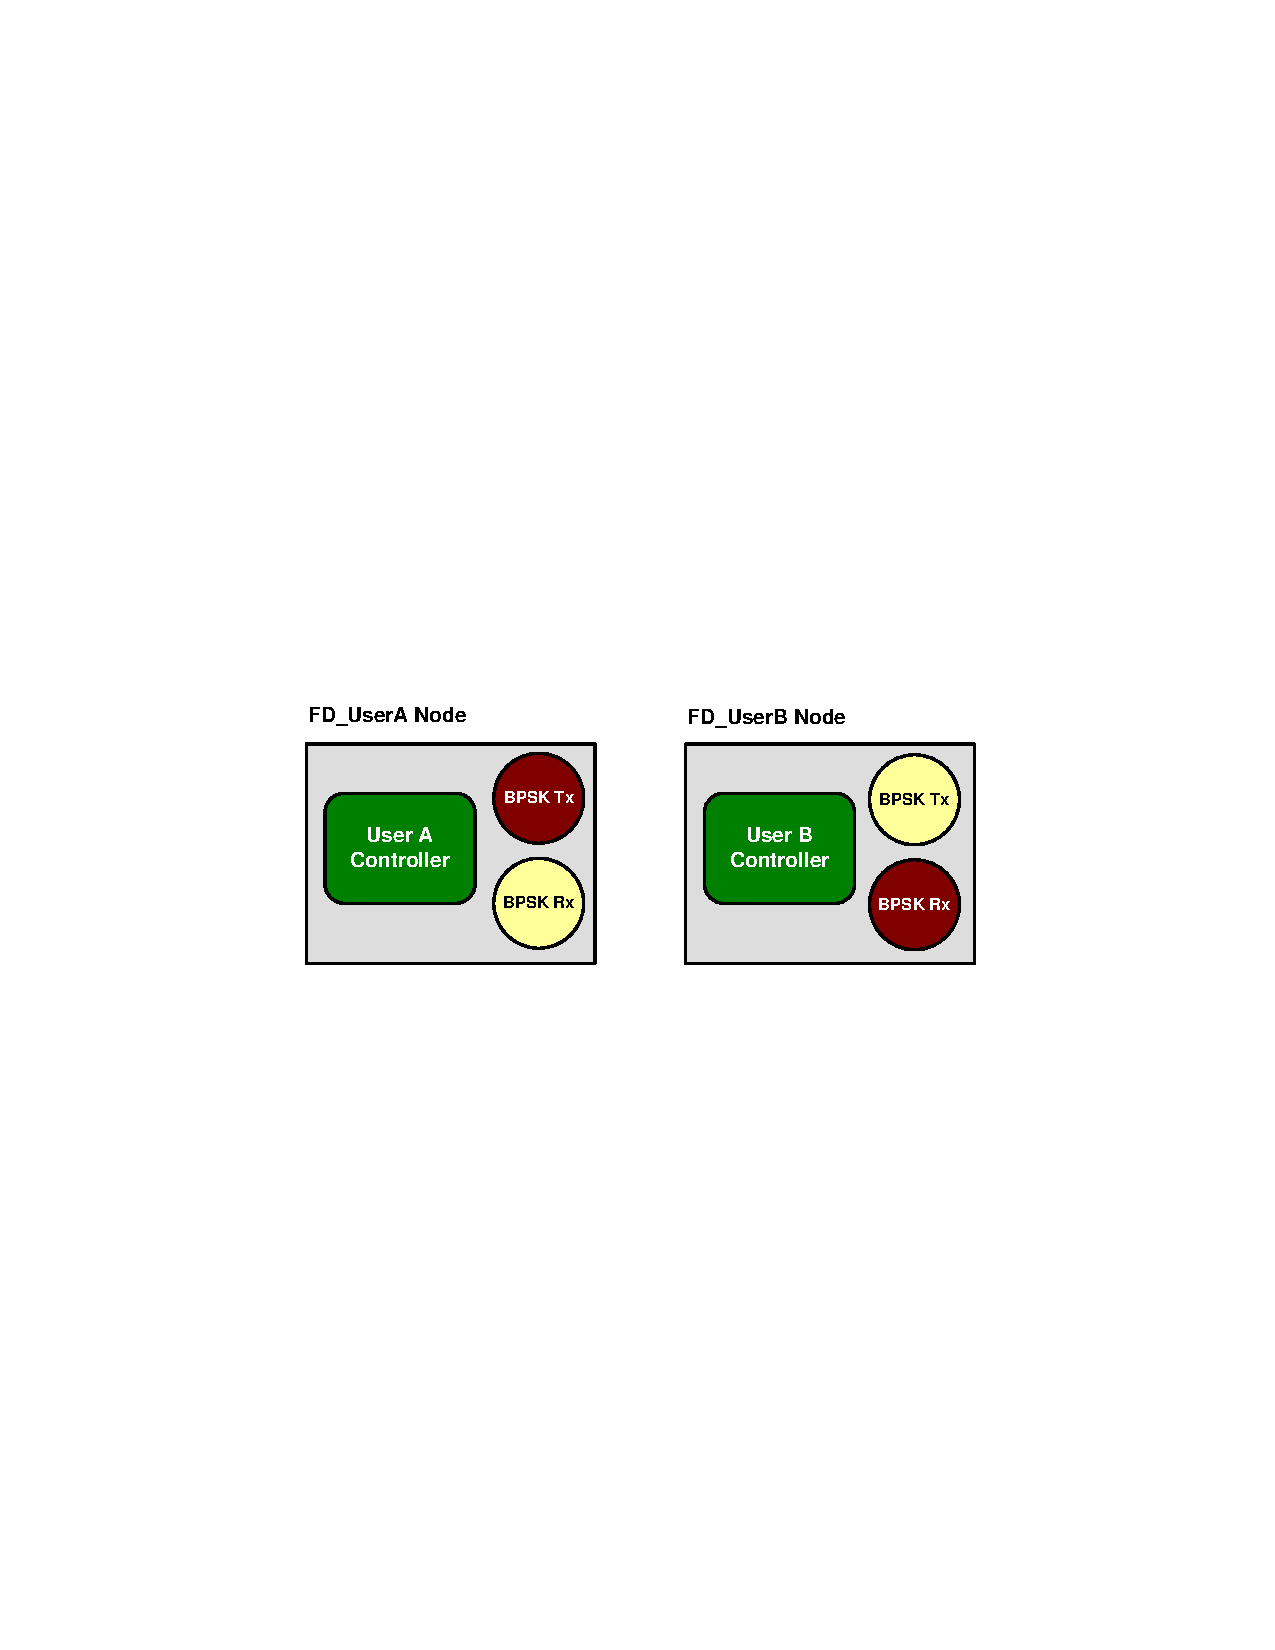
\includegraphics[width=3.5in]{figs/FD_Example}
\caption{Example full-duplex nodes} \label{fig:fdNodes}
\end{figure}

Figure \ref{fig:fdNodes} illustrates the object construction that is
required to implement this example.  As before, we will look at the
relevant portions of code that were required to implement this
example.  This time, however, we will concentrate mainly on the
differences between this example and the half-duplex example.

\subsubsection{FD\_BuildNodes.m}

In the half-duplex example from \S\ref{sec:hdExample}, we built two
modules and used copies of the two in each node. In the full-duplex
example, however, we need to build four nodes since the transmit and
receive frequencies are different.

The following fragments of code from
\verb+user_code/examples/BPSKNodes/FD_BuildNodes.m+ illustrate the important
differences between the half-duplex example and this example.  (Some
code has been snipped for clarity).

\begin{lstlisting}[name=fdBuildNodes][numbers=none]
function fdNodes = FD_BuildNodes
...
\end{lstlisting}
\begin{lstlisting}[name=fdBuildNodes, firstnumber=22][numbers=none]

% Define transmit/recieve modules

fd1_tx_mod_params.name = 'fd1_tx';
fd1_tx_mod_params.callbackFcn = @BPSK_Transmit;
fd1_tx_mod_params.fc = 2495e6;
fd1_tx_mod_params.type = 'transmitter';
...
\end{lstlisting}
\begin{lstlisting}[name=fdBuildNodes, firstnumber=40][numbers=none]
fd1_rx_mod_params.name = 'fd1_rx';
fd1_rx_mod_params.callbackFcn = @BPSK_Receive;
fd1_rx_mod_params.fc = 2495e6;
fd1_rx_mod_params.type = 'receiver';
...
\end{lstlisting}
\begin{lstlisting}[name=fdBuildNodes, firstnumber=56][numbers=none]
fd2_tx_mod_params.name = 'fd2_tx';
fd2_tx_mod_params.callbackFcn = @BPSK_Transmit;
fd2_tx_mod_params.fc = 1500e6;
fd2_tx_mod_params.type = 'transmitter';
...
\end{lstlisting}
\begin{lstlisting}[name=fdBuildNodes, firstnumber=71][numbers=none]
fd2_rx_mod_params.name = 'fd2_rx';
fd2_rx_mod_params.callbackFcn = @BPSK_Receive;
fd2_rx_mod_params.fc = 1500e6;
fd2_rx_mod_params.type = 'receiver';
...
\end{lstlisting}
\begin{lstlisting}[name=fdBuildNodes, firstnumber=87][numbers=none]
fd1_tx_mod = module(fd1_tx_mod_params);
fd1_rx_mod = module(fd1_rx_mod_params);
fd2_tx_mod = module(fd2_tx_mod_params);
fd2_rx_mod = module(fd2_rx_mod_params);
...
\end{lstlisting}

The code block above builds the four modules used in this example.
Note that these four modules have unique names.  The center
frequencies are set at 2495 MHz and 1500 MHz.  Also, the BPSK
receive and transmit functions were reused for this example.  The
next block of code in the file constructs the node objects.

\begin{lstlisting}[name=fdBuildNodes, firstnumber=93]
% Define nodes

FD_userA_node_params.name = 'FD_UserA';
FD_userA_node_params.location = [0 100 2];
FD_userA_node_params.velocity = [0 0 0];
FD_userA_node_params.controllerFcn = @FD_UserA_Controller;
FD_userA_node_params.modules = [fd1_tx_mod fd2_rx_mod];

FD_userB_node_params.name = 'FD_UserB';
FD_userB_node_params.location = [200 100 2];
FD_userB_node_params.velocity = [0 0 0];
FD_userB_node_params.controllerFcn = @FD_UserB_Controller;
FD_userB_node_params.modules = [fd2_tx_mod fd1_rx_mod];

FD_userA_node = node(FD_userA_node_params);
FD_userB_node = node(FD_userB_node_params);
\end{lstlisting}

The user parameters (shown below) are similar to the half-duplex
example.  For fun, \verb+nOversamp+ was increased to 3.  This
property is used within \verb+BPSK_Receive()+ and
\verb+BPSK_Transmit()+. Increasing \verb+nOversamp+ has the effect
of increasing the number of samples per bit for the full-duplex
transceivers.

\begin{lstlisting}[name=fdBuildNodes, firstnumber=111]
% Set user parameters

userParams.power = 10; % (Watts)
userParams.dataLen = 1800;
userParams.trainingLen = 200;
userParams.nOversamp = 3;
userParams.bitLen = userParams.dataLen+userParams.trainingLen;
userParams.blockLen = userParams.nOversamp*userParams.bitLen;

userParams.trainingSeq = rand(1,userParams.trainingLen)>.5;

userParams.nBlocksToSim = 10;
userParams.receivedBlocks = 0;
userParams.transmittedBlocks = 0;

userParams.txBits = zeros(userParams.nBlocksToSim,...
                          userParams.bitLen,'uint8');
userParams.rxBits = zeros(userParams.nBlocksToSim+1,...
                          userParams.bitLen,'uint8');

userParams.equalizerLen = 21;
userParams.equalizerDelay = 10;

userA_node = SetUserParams(FD_userA_node,userParams);
userB_node = SetUserParams(FD_userB_node,userParams);


% Put nodes into output array
fdNodes = [userA_node userB_node];
\end{lstlisting}

At the end of \verb+FD_BuildNodes.m+, the user parameters are saved
into the node object, and the nodes are returned in a 1x2 array.

\subsubsection{FD\_UserA\_Controller.m}

This section discusses the controller function for the full-duplex
node \verb+UserA+ (the controller for \verb+UserB+ is almost
identical).  This controller is noticeably different from the
controllers for the half-duplex examples.  In this example, nodes
both transmit and receive at the same time.  There are also some
additional states added for listening before the start of
communication.  In a more complicated example, this listening period
might be used to listen for a synchronization sequence or for
transmissions from possible interference sources.  Figure
\ref{fig:fdState} shows the state diagram for the controller.

\begin{figure}[h]
\centering
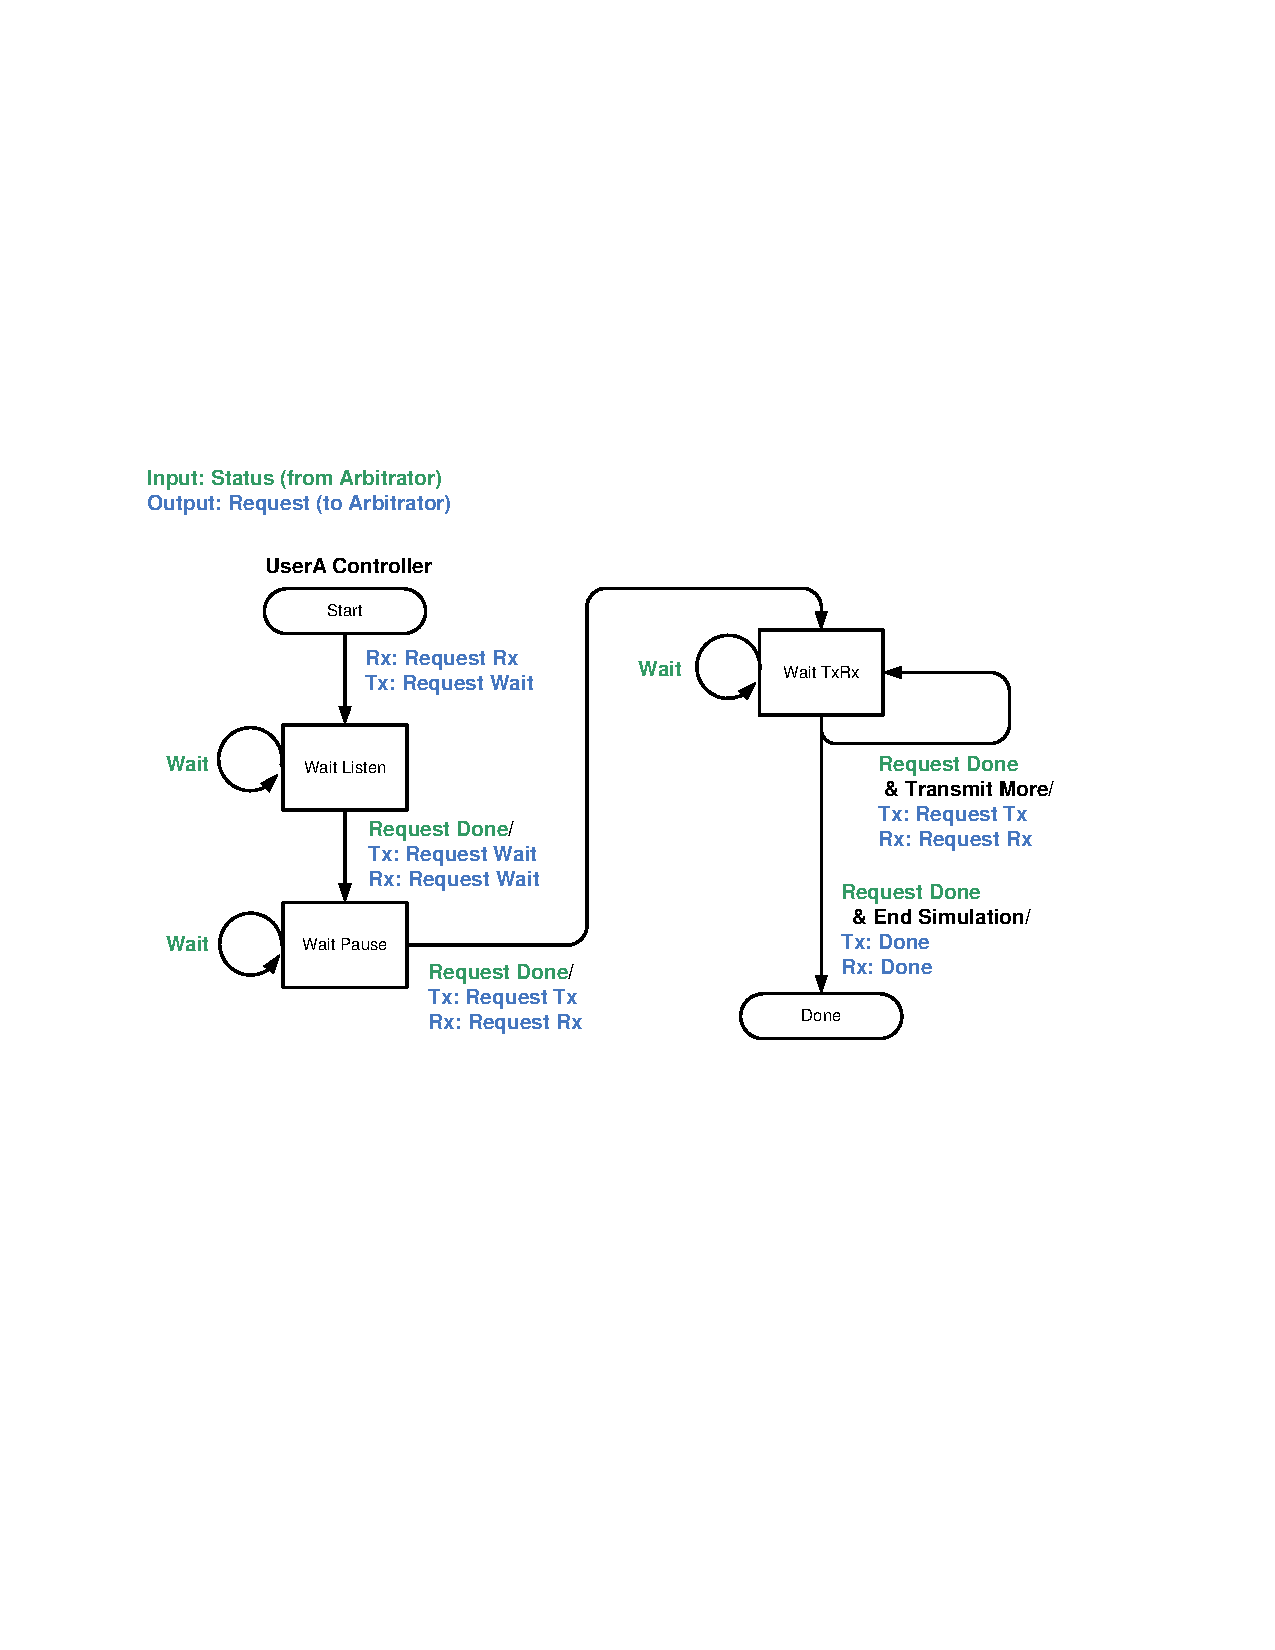
\includegraphics[width=5in]{figs/FD_State_Diagram}
\caption{State diagram for full-duplex controller function}
\label{fig:fdState}
\end{figure}

The corresponding MATLAB code for the state machine is shown in the
following listing.

\begin{lstlisting}[name=fdController][numbers=none]
function [nodeobj,status] = FD_UserA_Controller(nodeobj)
...
\end{lstlisting}
\begin{lstlisting}[name=fdController, firstnumber=24][numbers=none]
status = 'running';  % Default status

% Load user parameters
p = GetUserParams(nodeobj);

% Get current node state
currState = GetNodeState(nodeobj);

% State machine next-state and output "logic"
switch currState
    case 'start'
        % Listen for awhile
        nodeobj = SetModuleRequest(nodeobj,'fd2_rx','receive',p.blockLen);
        nodeobj = SetModuleRequest(nodeobj,'fd1_tx','wait',p.blockLen);
        nextState = 'listen_wait';
        
    case 'listen_wait'
        requests = CheckRequestFlags(nodeobj);
        if requests==0 
            % Pause for awhile
            nodeobj = SetModuleRequest(nodeobj,'fd2_rx','wait',250);
            nodeobj = SetModuleRequest(nodeobj,'fd1_tx','wait',250);
            
            nextState = 'pause_wait';
        else
            % Requests pending, wait
            nextState = 'listen_wait';
        end

    case 'pause_wait'
        requests = CheckRequestFlags(nodeobj);
        if requests==0
            % Start tx/rx
            nodeobj = SetModuleRequest(nodeobj,'fd2_rx',...
                                       'receive',p.blockLen);
            nodeobj = SetModuleRequest(nodeobj,'fd1_tx',...
                                       'transmit',p.blockLen);
            nextState = 'txrx_wait';
        else
            % All requests not satisfied, wait
            nextState = 'pause_wait';
        end
        
    case 'txrx_wait'
        requests = CheckRequestFlags(nodeobj);
        if requests==0
            if p.transmittedBlocks >= p.nBlocksToSim
                % Goto done
                nextState = 'done';
                nodeobj = SetModuleRequest(nodeobj,'fd2_rx','done');
                nodeobj = SetModuleRequest(nodeobj,'fd1_tx','done');
            else
                % Tx/Rx again
                nodeobj = SetModuleRequest(nodeobj,'fd2_rx',...
                                                'receive',p.blockLen);
                nodeobj = SetModuleRequest(nodeobj,'fd1_tx',...
                                                'transmit',p.blockLen);
                nextState = 'txrx_wait';
            end
        else
            % All requests not satisfied, wait
            nextState = 'txrx_wait';
        end
        
    case 'done'
        % Done!
        nextState = 'done';
        status = 'done';
                
    otherwise
        error(sprintf('Unknown state: %s',currState));
end

% Set next state
nodeobj = SetNodeState(nodeobj,nextState);

% Store possibly modified user params
nodeobj = SetUserParams(nodeobj,p);
\end{lstlisting}

The structure of the code is similar to the previous half-duplex
example.  The state machine is implemented as a large switch
statement.  The state and user parameters are loaded at the
beginning of the function, and saved at the end.  This general
structure should be flexible enough to implement any controller
function.

\subsection{The Interference Sources}
\label{sec:interference_source}
The example scenario includes two interference sources: one in the
FM radio band (99.5 MHz), and one in the ISM band (2495 MHz). The FM
interferer transmits complex colored gaussian noise. The ISM
interferer transmits complex white gaussian noise. Interference
sources are transmit-only, so contain only a transmit module. Figure
\ref{fig:interfNodes} shows a diagram of the example interference
nodes.

\begin{figure}[h]
\centering
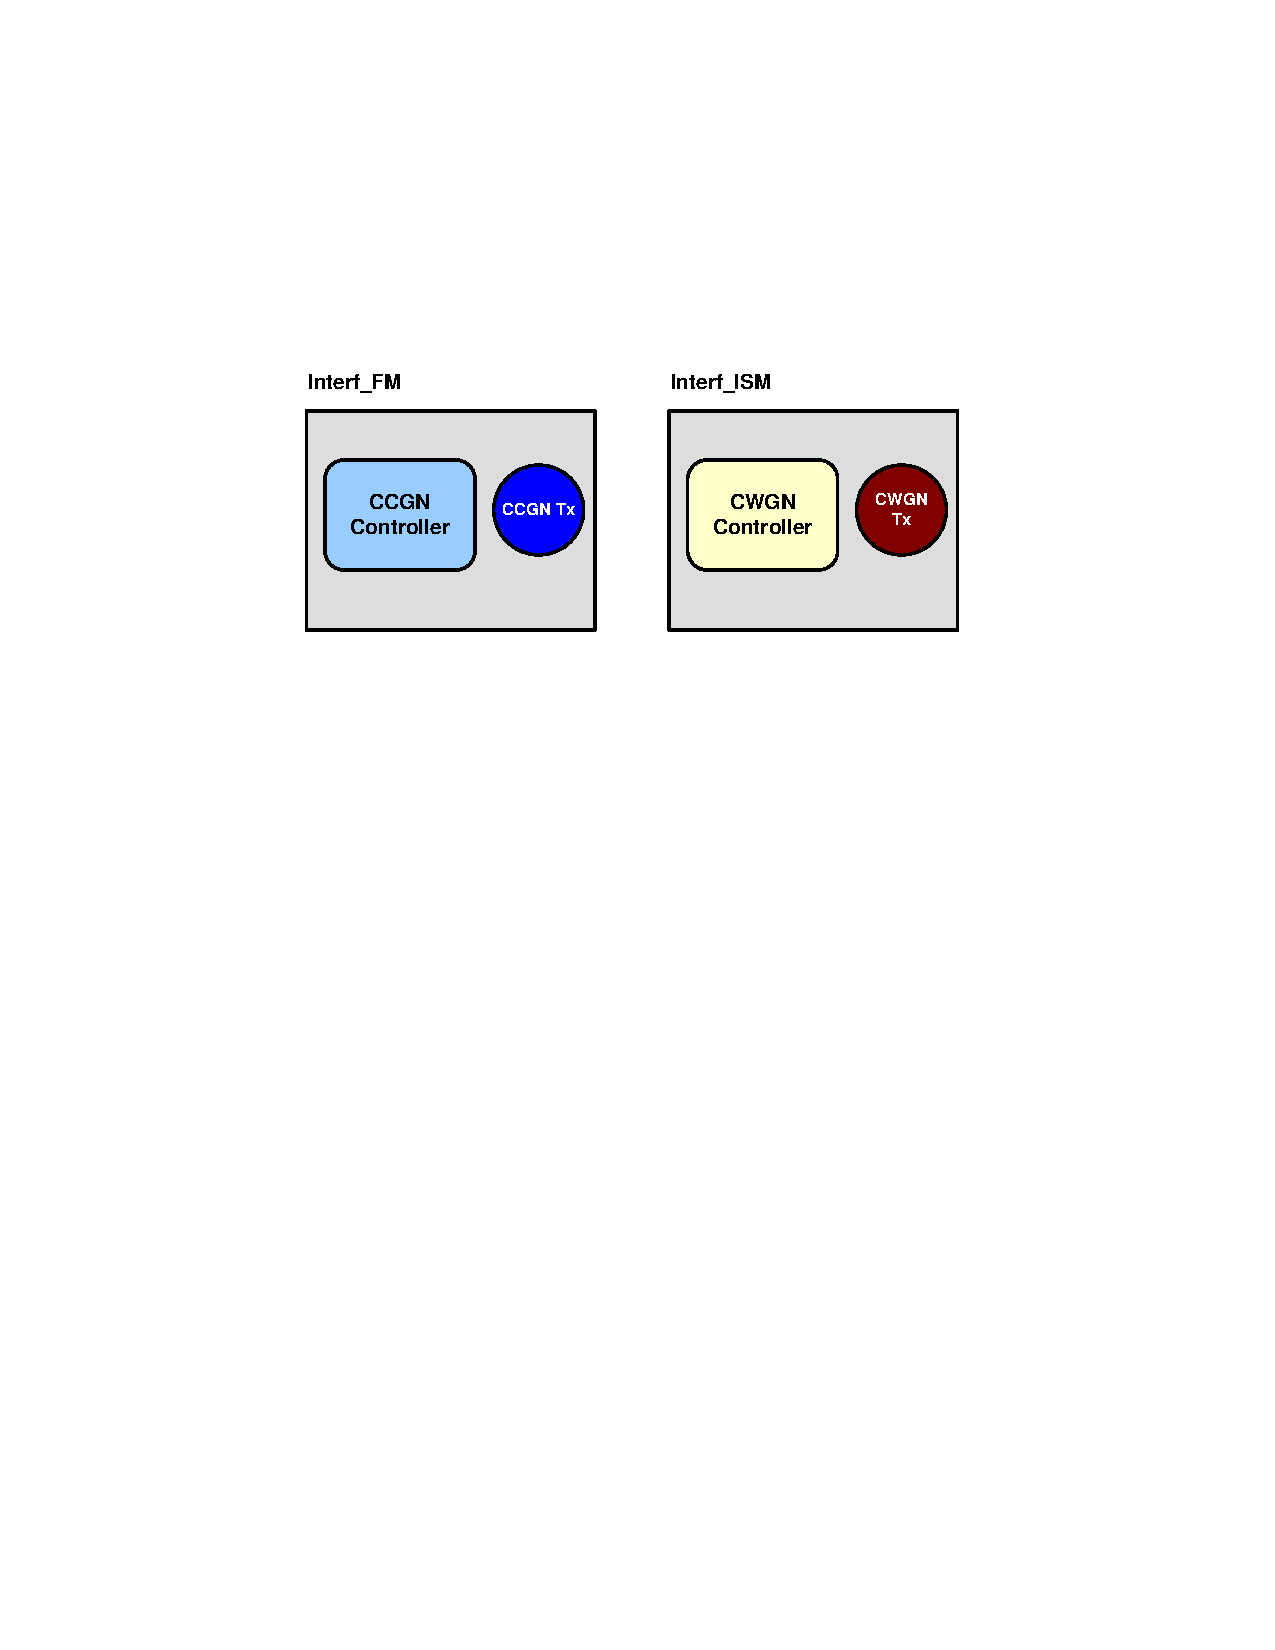
\includegraphics[width=3.5in]{figs/Interf_Example}
\caption{Example interference nodes} \label{fig:interfNodes}
\end{figure}

There are five files in the \verb+user_code/examples/InterferenceNodes+
directory. The interference sources are constructed in
\verb+Ex_BuildInterference.m+.  \verb+CCGN_Controller.m+ and
\verb+CWGN_Controller.m+ define the controller functions.
\verb+CWGN_Transmit.m+ and \verb+CCGN_Transmit.m+ define the
transmit functions. It is left to the interested reader to examine
the source code on her own.

One thing to note within the controller functions is that the
modules are never marked as ``done'' (by using
\verb+SetModuleRequest(...,'done')+). This is so that the simulation
will stall if there are not enough interference samples created.

\subsection{The LL MIMO Nodes}\label{sec:llmimoNodes}

The final nodes included in the canonical example are the Lincoln
Laboratory MIMO nodes.  These demonstrate the simulation of a very
basic MIMO (Multiple Input Multiple Output) communication system
Files related to these nodes can be found in the 
\verb+user_code/examples/MIMONodes+ directory.
This example also makes use of the special ``genie'' channel for
quickly implementing a reverse link, and defines custom plots for
the timing diagram.

\begin{figure}[h]
\centering
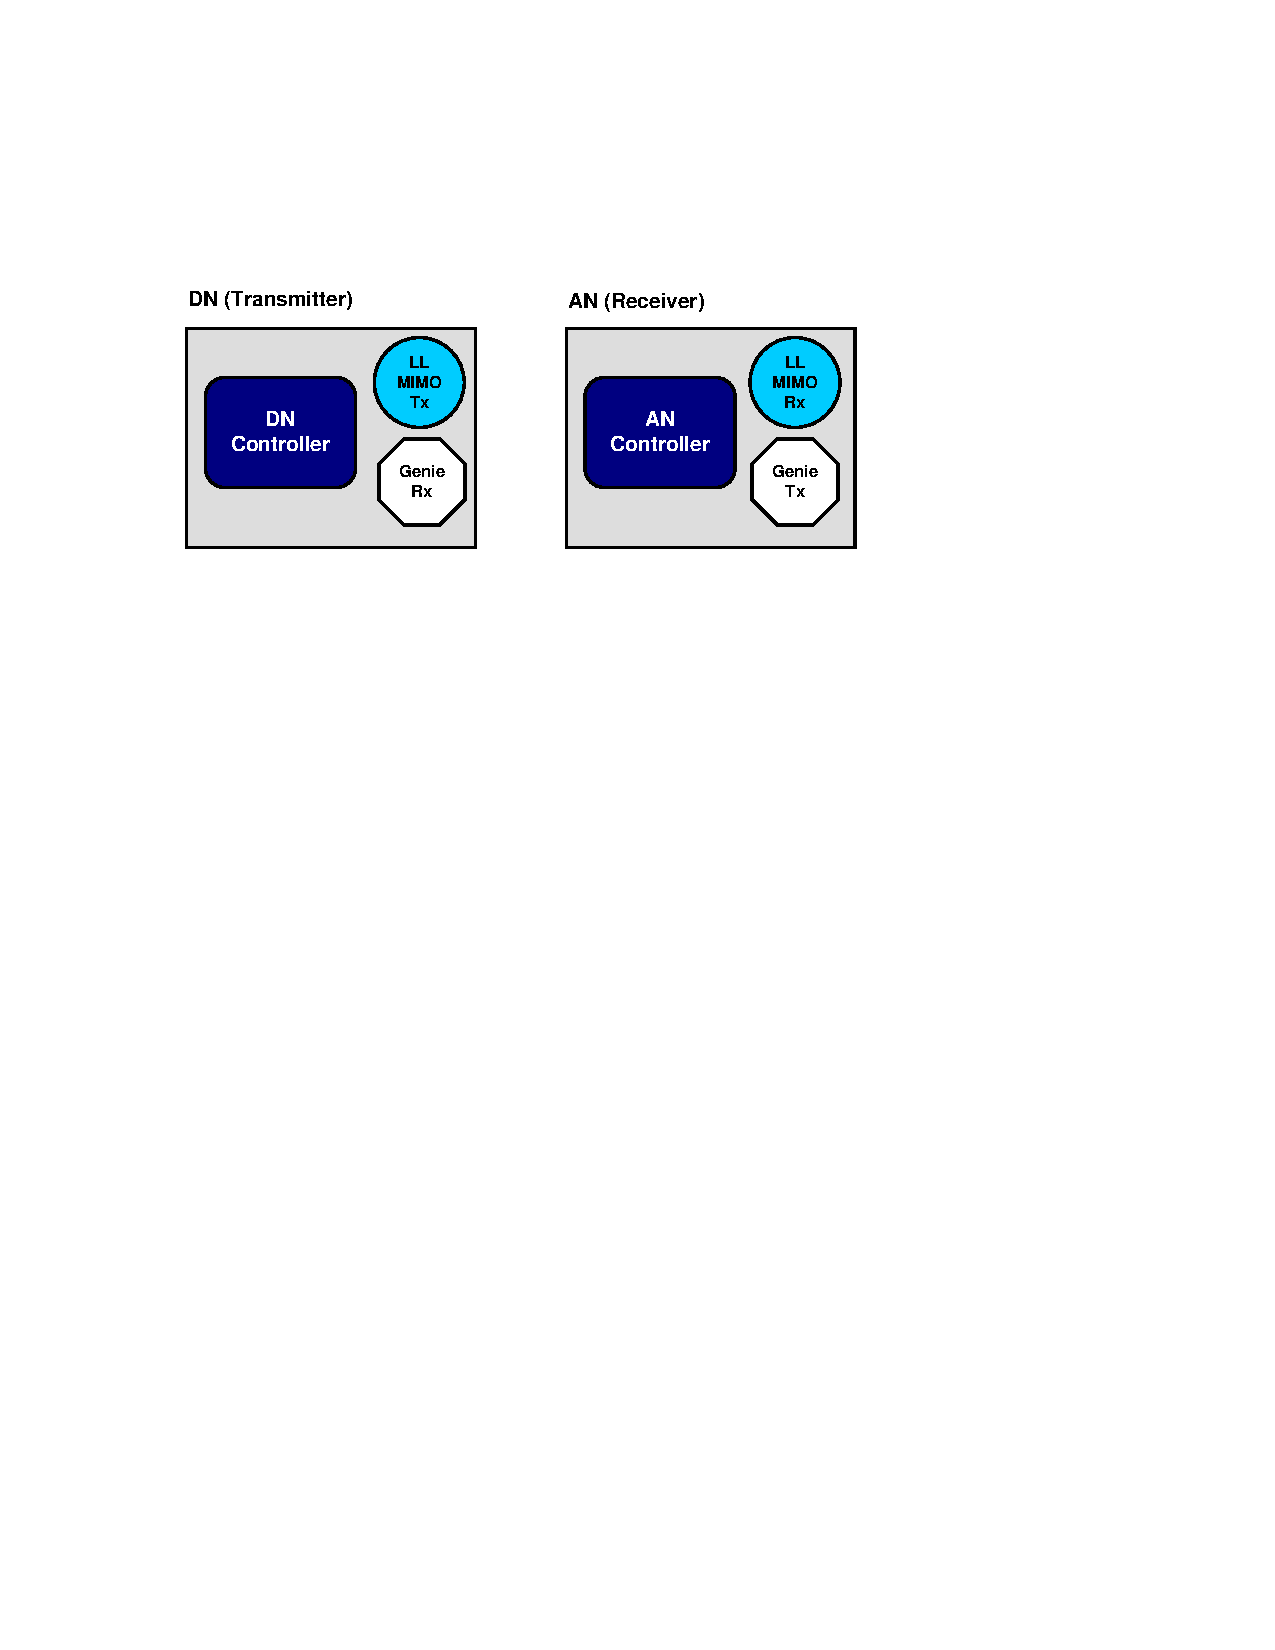
\includegraphics[width=3.5in]{figs/LL_MIMO_Example}
\caption{LL MIMO nodes} \label{fig:llmimoNodes}
\end{figure}

Figure \ref{fig:llmimoNodes} shows the node structure for the LL
MIMO nodes.% 
%The nodes are named \verb+DN+ and \verb+AN+ for
%historical reasons.  These were the names given to the transmitter
%and receiver, respectively, in Cogcom.  
\verb+DN+ is an acronym for ``disadvantaged node'', and \verb+AN+ stands for ``advantaged node''.  The genie channel is implemented by including genie
modules. The genie modules are shown as octagons in the figure.

\subsubsection{LLMimo\_BuildNodes.m}

The LL MIMO nodes are constructed in
\verb+LLMimo_BuildNodes.m+.  The structure of the file
should be very familiar to anyone who has read the previous sections
explaining the half-duplex and full-duplex examples.  The only
differences are the inclusion of the genie modules, and the way the
user parameters are defined.  Portions of the file are explained below.

\begin{lstlisting}[name=llmimoBuild]
function LLMimoNodes = LLMimo_BuildNodes(range, envType)

% Function LLMimo_BuildNodes.m:
% Example function/script for building user nodes with common
% transmit/receive modules and user parameters.
% 
% USAGE: LLMimoNodes = LLMimo_BuildNodes
%
% Input arguments:
%  range        (string) range is 'short', 'short-medium', 'medium', or 'long'
%  envType      (string) Environment type: 'rural', 'suburban', or 'urban'
%
% Output arguments:
%  LLMimoNodes  (1xN Node obj array) Newly-created user nodes
%

%%%%%%%%%%%%%%%%%%%%%%%%%%%%%%%%%%%%%%%%%%%%%%%%%%%%%%%%%%%%%%%%%
% Copyright (c) 2006-2016 Massachusetts Institute of Technology %
% All rights reserved.   See software license below.            %
%%%%%%%%%%%%%%%%%%%%%%%%%%%%%%%%%%%%%%%%%%%%%%%%%%%%%%%%%%%%%%%%%

% Define transmit/receive modules

tx_mod_params.name = 'LLmimo_tx';
tx_mod_params.callbackFcn = @LLMimo_Transmit;
tx_mod_params.fc = 850e6;
tx_mod_params.type = 'transmitter';
tx_mod_params.loError = 0;
tx_mod_params.antType = {'dipole_halfWavelength'};
tx_mod_params.antPosition = [0 -5 0;
                             0 -4 0;
                             0 -3 0;
                             0 -2 0;
                             0 -1 0;
                             0 0 0;
                             0 1 0;
                             0 2 0;
                             0 3 0;
                             0 4 0]*3e8/tx_mod_params.fc;
tx_mod_params.antPolarization = {'v'};
tx_mod_params.antAzimuth = [0];
tx_mod_params.antElevation = [0];
tx_mod_params.exteriorWallMaterial = 'none';
tx_mod_params.distToExteriorWall = [0];
tx_mod_params.exteriorBldgAngle = [0];
tx_mod_params.numInteriorWalls = [0];


rx_mod_params.name = 'LLmimo_rx';
rx_mod_params.callbackFcn = @LLMimo_Receive;
rx_mod_params.TDCallbackFcn = @LLMimo_Rx_TDCallback;
rx_mod_params.fc = 850e6;
rx_mod_params.type = 'receiver';
rx_mod_params.loError = 0;
rx_mod_params.noiseFigure = 6; % (dB) noise figure of receiver
rx_mod_params.antType = {'dipole_halfWavelength'};
rx_mod_params.antPosition = [0 -4 0;
                             0 -2 0;
                             0 0 0;
                             0 2 0]*3e8/rx_mod_params.fc;
rx_mod_params.antPolarization = {'v'};
rx_mod_params.antAzimuth = [0];
rx_mod_params.antElevation = [0];
rx_mod_params.exteriorWallMaterial = 'none';
rx_mod_params.distToExteriorWall = [0];
rx_mod_params.exteriorBldgAngle = [0];
rx_mod_params.numInteriorWalls = [0];


tx_mod = module(tx_mod_params);
rx_mod = module(rx_mod_params);

\end{lstlisting}

Module objects are constructed in the normal fashion.  However,
since this example involves a MIMO transmitter and receiver, the
antenna position, \verb+antPosition+ (line 30 and 57), is a
2-dimensional matrix rather than a single vector.\footnote{Please
refer to the reference section for more details.}  Also,
\verb+rx_mod_params.TDCallbackFcn+ has been defined on line 51.  The
function that it points to, \verb+LLMIMO_Rx_TDCallback+ is a custom
plot for the timing diagram callback.

\begin{lstlisting}[name=llmimoBuild]
% Create genie modules
tx_gen.name = 'genie_tx';
tx_gen.type = 'transmitter';

rx_gen.name = 'genie_rx';
rx_gen.type = 'receiver';

gen_tx_mod = module(tx_gen,1);
gen_rx_mod = module(rx_gen,1);


\end{lstlisting}

The section above creates the genie receive and transmit modules.
Genie modules transfer information without actually sending an
analog signal through the environment.  Instead, data sent from one
genie module ``magically'' appears at another.  Unlike normal
modules, no functions need to be written to define the
modulation/demodulation schemes.  Note that a genie transmit module can multi-cast a message to several genie receive modules.

The genie modules are defined by a name and a type (transmitter or
receiver). To build a genie module, simply include an extra argument
in the call to the module constructor (lines 80-81).  This extra
argument is the ``genie flag''.  It instructs the constructor to
make a genie module.

\begin{lstlisting}[name=llmimoBuild]
% Define nodes

DN_node_params.name = 'DN';
switch lower(range)
    case 'short'
        DN_node_params.location = [1.0e3 0 3];
    case 'short-medium'
        DN_node_params.location = [2.5e3 0 3];
    case 'medium'
        DN_node_params.location = [5.0e3 0 3];
    case 'long'
        DN_node_params.location = [1.0e4 0 3];
    otherwise
        error('Incorrect range case')
end
DN_node_params.velocity = [0 0 0];
DN_node_params.controllerFcn = @LLMimo_DN_Controller;
DN_node_params.modules = [tx_mod gen_rx_mod];

AN_node_params.name = 'AN';
switch lower(envType)
    case 'rural'
        AN_node_params.location = [0 0 100];
    case 'suburban'
        AN_node_params.location = [0 0 30];
    case 'urban'
        AN_node_params.location = [0 0 30];
    otherwise
        error('Incorrect environment type!')
end
AN_node_params.velocity = [0 0 0];
AN_node_params.controllerFcn = @LLMimo_AN_Controller;
AN_node_params.modules = [rx_mod gen_tx_mod];

DN_node = node(DN_node_params);
AN_node = node(AN_node_params);


\end{lstlisting}

The code block above builds the nodes.  The genie module is included
in the array of modules just like a normal module.  The genie
modules are used in the controller function similar to a normal
module, but using different function calls.  This is discussed in
more detail later.  The DN location is specified by the function input \verb+range+ and the AN location is specified by the function input \verb+envType+.

User parameters are defined by populating a struct with field names
and values just as before.  In this example, however, one node only
transmits, while the other only receives.  As a result, some
parameters, such as the training sequence, are shared, while other
parameters, such as the transmit bits, are not.

\begin{lstlisting}[name=llmimoBuild]
% Define shared parameters (packet definition)
sharedParams.noiseLen = 100;
sharedParams.hTrainingLen = 100;
sharedParams.hTrainingSeq = rand(GetNumAnts(tx_mod),...
    sharedParams.hTrainingLen)>.5;
sharedParams.trainingLen = 100;
sharedParams.trainingSeq = rand(1,sharedParams.trainingLen)>.5;
sharedParams.infoLen = 512;
sharedParams.spreadRatio = 5;
sharedParams.nOversamp = 3;
sharedParams.blockLen = sharedParams.nOversamp*...
    (sharedParams.noiseLen+sharedParams.hTrainingLen+...
     sharedParams.trainingLen+sharedParams.spreadRatio...
     *sharedParams.infoLen);
sharedParams.nBlocksToSim = 8;

\end{lstlisting}

The shared parameters, shown above, include all the information that
is required to synchronize between the two radios.  These parameters
define the packet structure and the training sequences.  The number
of packets to simulate is also defined here (line 136).

\begin{lstlisting}[name=llmimoBuild]
% DN-specific (Transmitter) parameters
dnParams.transmittedBlocks = 0;
dnParams.txPower = 1; % (Watts)
dnParams.targDomAtten = 2;
dnParams.infoSourceFilename = './user_code/examples/MIMONodes/testdata_long.dat';
dnParams.infoSourceFID = [];
dnParams.infoBits = [];
dnParams.txBitsFilename = '';
dnParams.txBitsFID = [];
dnParams.getFromRx = [];

\end{lstlisting}

The transmitter (\verb+DN+) in this example does not generate data
randomly as in previous examples.  Instead, it reads binary data
from a file.  This file is specified as a parameter named
\verb+infoSourceFilename+ (line 142).  When running, the controller
function will read a block of data from file and put it into
\verb+infoBits+. \verb+LLMimo_Transmit()+ will then modulate this
data for transmission. The field \verb+infoSourceFID+ will be used
to hold a pointer to the \verb+testdata_long.dat+ once it is opened.

While it's possible to read the entire datafile and put the bits
into \verb+infoBits+, this is not suggested.  Doing so will use a
lot of computer memory and incur a large amount of overhead during
function calls. The simulation will run slowly.\footnote{MATLAB
passes a \emph{copy} of the node object during function calls. There
is no such thing as passing objects by reference.}

\verb+LLMimo_Transmit()+ will save all transmitted bits into the
file to be specified in the field \verb+txBitsFilename+.  This is
used later for calculating the BER.  In previous examples, bits were
stored directly in the node.  However, this example is sufficiently
large that it is more computationally efficient to write the
information to file for the same reasons explained above.

The field \verb+getFromRx+ is a struct.  It is used to hold data
received by the genie receive module.  The information is passed
from the genie receive module, to the controller, and then to the
transmit function \verb+LLMimo_Transmit()+ in the transmit module
\verb+LLMimo_Tx+.  This process can be better understood by seeing
it in the controller function in the following section.

\begin{lstlisting}[name=llmimoBuild]
% AN-specific (Receiver) parameters
anParams.receivedBlocks = 0;
anParams.epsilon = 10^-5;
anParams.lagRange = [-50:5];
anParams.rxBitsFilename = '';
anParams.rxBitsFID = [];
anParams.passToTx = [];

\end{lstlisting}

Parameters for the receiver are defined in the fragment of code
shown above.  \verb+epsilon+ and \verb+lagRange+ define parameters
that are used by the STAP receiver in \verb+LLMimo_Receive()+.  The
demodulated bits are stored into the file specified by
\verb+rxBitsFilename+.

The field \verb+passToTx+ is used to hold information being passed
back to the \verb+DN+.  Data stored here by \verb+LLMimo_Receive()+
is copied into the genie transmit module by the AN controller
function and sent to the DN genie receive module (or to others if multi-cast).

\begin{lstlisting}[name=llmimoBuild]
% Save parameters within nodes
dnParams = StructMerge(dnParams,sharedParams);
DN_node = SetUserParams(DN_node,dnParams);

anParams = StructMerge(anParams,sharedParams);
AN_node = SetUserParams(AN_node,anParams);


% Put user nodes into array
LLMimoNodes = [DN_node AN_node];
\end{lstlisting}

\verb+StructMerge()+ is a utility function that merges the fields of
two different structs into one.  The merged parameters are stored
into the node objects and the node objects are returned as an array.

\subsubsection{LLMimo\_Transmit.m and LLMIMO\_Receive.m}

The transmit and receive function for the LL MIMO example implement
a simple MIMO link.  The transmit function uses a very simple
repetition code, and the signal is BPSK encoded and resampled
without pulse shaping.  The receiver uses a STAP beamformer. In
terms of programming, only one line is worth noting.

\begin{lstlisting}[name=llmimoReceive,firstnumber=71]
% Save received bits to file for comparison with received bits
[count,fPtr] = WriteBitBlock(p.rxBitsFID,demodBits);
\end{lstlisting}

The code above from \verb+LLMimo_Receive.m+ shows a call to the
function \verb+WriteBitBlock()+.  This function saves the
demodulated bits to file for calculation of the BER.  There is a
corresponding line of code in \verb+LLMimo_Transmit.m+ that writes
transmitted bits to file.  The files are initialized at startup by
the controller function.

\subsubsection{LLMimo\_AN\_Controller.m and LLMimo\_DN\_Controller.m}

The structure of the controller function should be familiar, by now.
However, since this is the first example that incorporates the use
of the genie modules, it may be useful to examine the details.

\begin{figure}[h]
\centering
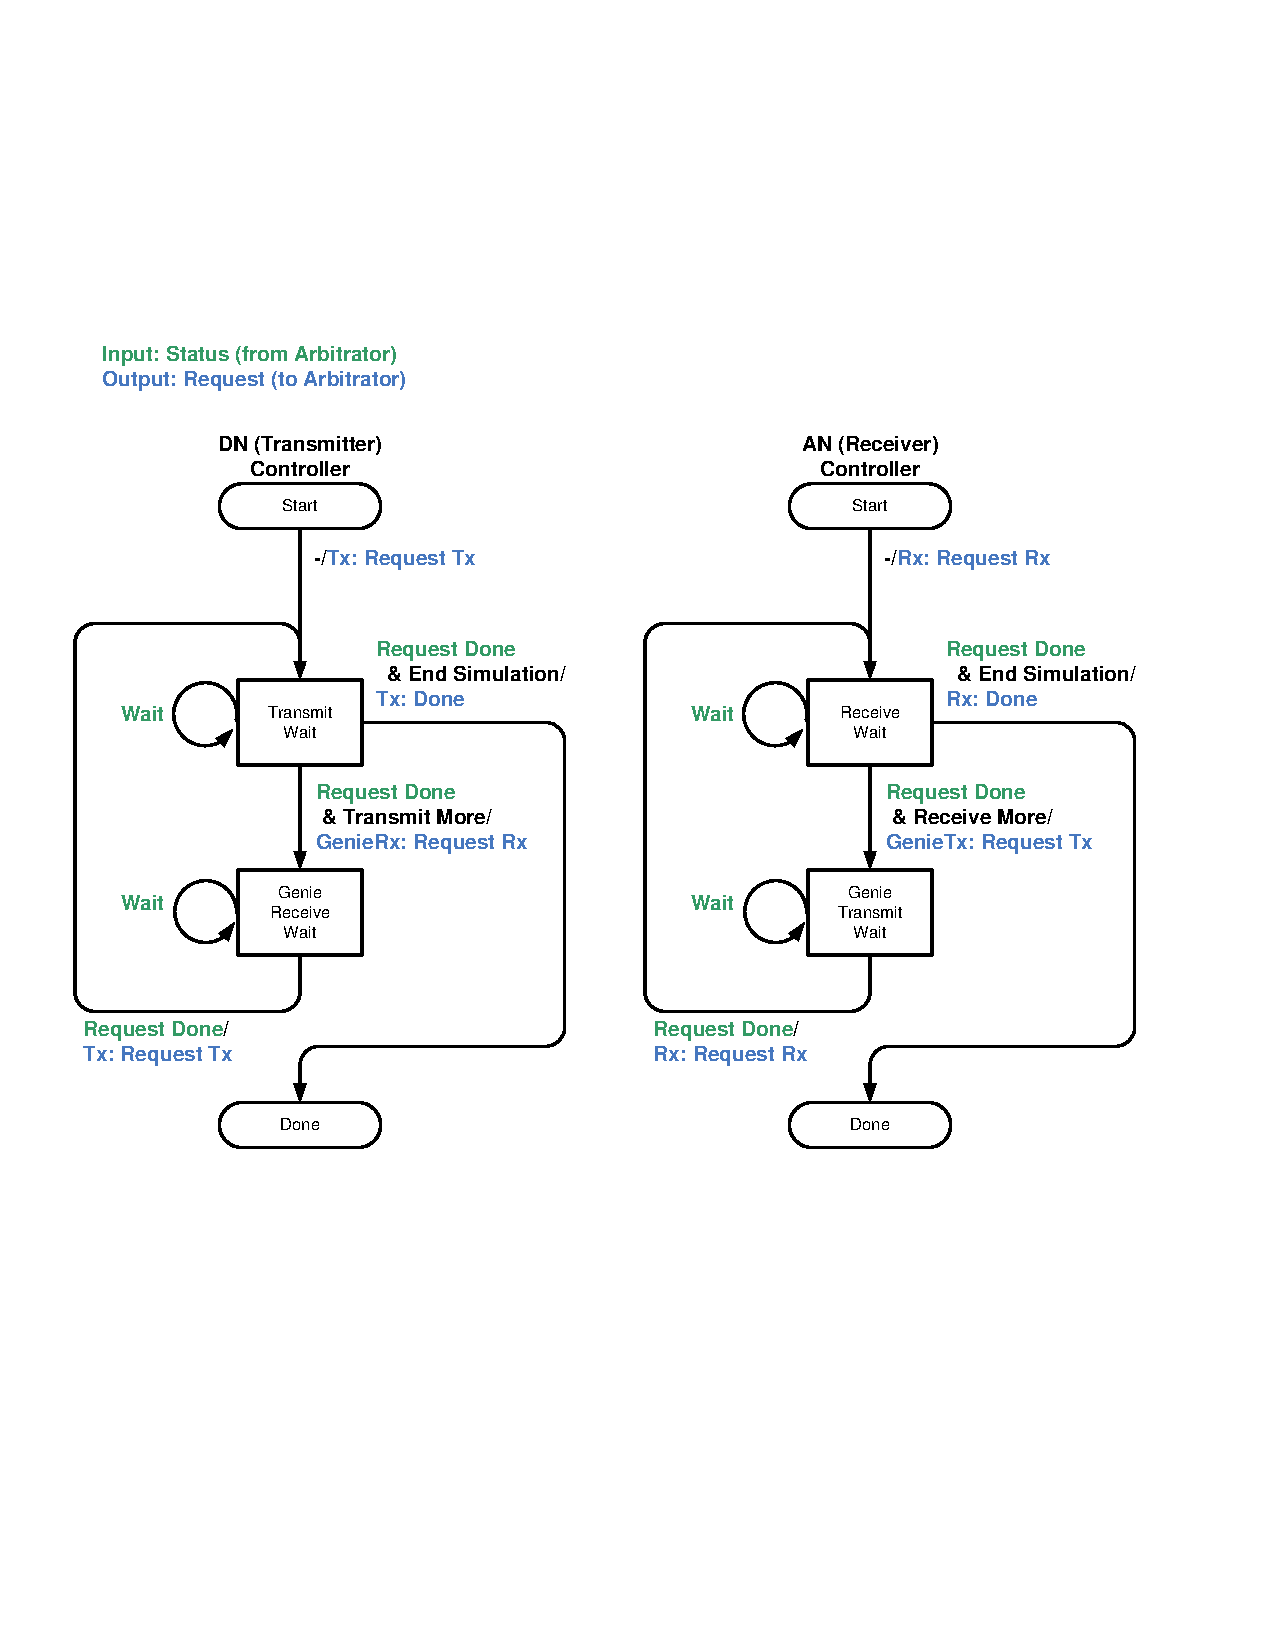
\includegraphics[width=5in]{figs/LL_MIMO_State_Diagram}
\caption{State diagrams for LL MIMO controllers}
\label{fig:llmimoState}
\end{figure}

Figure \ref{fig:llmimoState} shows the state diagrams for the
controller functions.  Note that neither the LL MIMO transmit module
nor the LL MIMO receive module are ever placed into a wait state.
This is because the genie module is special.  It transmits
information in zero time.  As a result, a separate state is required
in the controller (as in the half-duplex example), but there is no
need to instruct the transmit/receive modules to wait.

Requests for genie modules to transmit or receive are made using the
functions \verb+SetGenieTxRequest()+ and \verb+SetGenieRxRequest()+.
Data is loaded into or read from the modules using
\verb+ReadGenieInfo()+ and \verb+WriteGenieInfo()+. The code
fragment below from \verb+LLMimo_AN_Controller.m+ illustrates how
the functions are used to initiate a genie transmission.

\begin{lstlisting}[name=llmimoANCon,firstnumber=53]
   % Put send data into module's genie queue
   nodeobj = WriteGenieInfo(nodeobj,'genie_tx',p.passToTx);

   % Request send through genie channel to DN's genie receive
   nodeobj = SetGenieTxRequest(nodeobj,'genie_tx','DN','genie_rx');
   ...
\end{lstlisting}

In additional to the node object and module name,
\verb+SetGenieTxRequest()+ takes the destination node and module
name.  This is required because it is possible for a genie transmit
module to send to any genie receive module in a scenario.   To multi-cast to multiple genie modules, the \verb+toNodeName+ and \verb+toModName+ can be (equal sized) cell arrays.  Data is delivered to the genie queue for each specified node/module address.

Similarly, the code snippets below from
\verb+LLMimo_DN_Controller.m+ show the code required to receive from
a genie channel.

\begin{lstlisting}[name=llmimoDNCon,firstnumber=62]
    ...
    % Transmission done, receive feedback info from genie channel
    nodeobj = SetGenieRxRequest(nodeobj,'genie_rx');
\end{lstlisting}

\begin{lstlisting}[name=llmimoDNCon,firstnumber=72]
    ...
    requests = CheckRequestFlags(nodeobj);
    if requests==0
        % Got feedback, copy received info into user params
        [nodeobj,p.getFromRx] = ReadGenieInfo(nodeobj,'genie_rx');
    ...
\end{lstlisting}

This example provided a very brief overview to how genie channels
are used. It should be enough information to get started.

\subsubsection{LLMimo\_CalcBER.m}

The LL MIMO example saves the transmitted and received bits to file
rather than within the node object.  This was done to conserve
memory (at the expense of disk space).  As a result, calculating the
BER requires reading data from file.  The code block below from
\verb+LLMimo_CalcBER.m+ illustrates this process using the functions
provided with LLAMAComm.  \verb+ReadBitBlock()+ reads bits from
files that were written by \verb+WriteBitBlock()+ (which is called
from within \verb+LLMimo_Transmit()+ and \verb+LLMimo_Receive()+).

\begin{lstlisting}[name=llmimoCalcBER]
function ber = LLMimo_CalcBER(nodes)

% Function user.LL/LLMimo_CalcBER.m:
% Calculates the Bit-Error Rate for the LLMimo example
%
% USAGE:  ber = LLMimo_CalcBER(nodes)
%
% Input arguments:
%  nodes     (node obj array, 1xN) Node objects
%
% Output arguments:
%  ber       (1x1) BER for DN->AN link
%

%%%%%%%%%%%%%%%%%%%%%%%%%%%%%%%%%%%%%%%%%%%%%%%%%%%%%%%%%%%%%%%%%
% Copyright (c) 2006-2016 Massachusetts Institute of Technology %
% All rights reserved.   See software license below.            %
%%%%%%%%%%%%%%%%%%%%%%%%%%%%%%%%%%%%%%%%%%%%%%%%%%%%%%%%%%%%%%%%%


% Extract user parameters
pAN = GetUserParams(FindNode(nodes,'AN'));
pDN = GetUserParams(FindNode(nodes,'DN'));

% Open saved files for reading
ANfid = OpenBitFile(pAN.rxBitsFilename);
DNfid = OpenBitFile(pDN.txBitsFilename);

% Loop through blocks
ANfPtr = 0;
DNfPtr = 0;
errCount = 0;
bitCount = 0;
while(1)

    [ANbits,ANfPtr] = ReadBitBlock(ANfid,ANfPtr);
    [DNbits,DNfPtr] = ReadBitBlock(DNfid,DNfPtr);

    if isempty(ANbits) && isempty(DNbits)
        % Done with files
        break;

    elseif ~isempty(ANbits) && ~isempty(DNbits)
        % Compare data
        errs = find(xor(ANbits,DNbits));

        % Count errors and bits
        errCount = errCount+length(errs);
        bitCount = bitCount+size(ANbits,2);

    else
        error('Bit files have unequal length!');
    end
end

% Calculate BER
ber = errCount/bitCount;

% Print results to screen
fprintf('LL MIMO example, DN->AN BER: %f\n',ber);

% Close opened files
fclose(ANfid);
fclose(DNfid);
\end{lstlisting}


\subsection{The Example Environment} \label{sec:exampleEnv}

The example simulation is run using an example environment created
in \verb+user_code/examples/Ex_BuildEnvironment.m+.  The code sets some
properties and builds an environment object.  Details about the environment
properties can be found in Chapter \ref{chp:reference}.

\begin{lstlisting}[name=exEnv]
function env = Ex_BuildEnvironment

% Function Ex_BuildEnvironment.m:
% Builds an example rural environment object.
%
% USAGE: env = Ex_BuildEnvironment
%
% Input args:
%  -none-
%
% Output arguments:
%  env    (environment object) New environment object
%

%%%%%%%%%%%%%%%%%%%%%%%%%%%%%%%%%%%%%%%%%%%%%%%%%%%%%%%%%%%%%%%%%
% Copyright (c) 2006-2016 Massachusetts Institute of Technology %
% All rights reserved.   See software license below.            %
%%%%%%%%%%%%%%%%%%%%%%%%%%%%%%%%%%%%%%%%%%%%%%%%%%%%%%%%%%%%%%%%%

test_env_params.envType = 'rural';
test_env_params.propParams.delaySpread = .2e-6;  % sec
test_env_params.propParams.velocitySpread = 0.1;  % m/s
test_env_params.propParams.alpha = 0.5;
test_env_params.propParams.longestCoherBlock = 1;
test_env_params.propParams.stfcsChannelOversamp = 3;
test_env_params.propParams.wssusChannelTapSpacing = []; % samples
test_env_params.propParams.los_dist = 10;             % m
test_env_params.building.avgRoofHeight = 4;
env = environment(test_env_params);
\end{lstlisting}

\subsection{The Start Script}

The start script is responsible for setting up the required paths,
calling the proper build files, and starting the simulation by
calling the \verb+Main()+ function.  The contents of the
\verb+StartExample.m+ script are shown below.

\begin{lstlisting}[name=startExample]
% Script StartExample.m:
% The start script sets up the MATLAB path, calls user functions 
% to set up the simulation universe, and starts the simulation.  
% When the simulation is complete, user-defined functions can be 
% called to analyze the results.
%
% This script runs the example described in the documentation:
%    Easy rural environment
%    2 Half-duplex nodes transmitting BPSK in the FM band
%    2 Full-duplex nodes transmitting BPSK in GlobalStar/ISM
%    1 Complex white gaussian noise interferer in the ISM band
%    1 complex colored gaussian noise interferer in the FM band
%    2 LL Mimo nodes (forward link with genie reverse link)
%
\end{lstlisting}
\begin{lstlisting}[name=startExample,firstnumber=21]
% Add required directories containing simulator functions 
% to the MATLAB search path
SetupPaths;

% Paths to user-defined functions
addpath ./examples
addpath ./examples/BPSKNodes
addpath ./examples/MIMONodes
addpath ./examples/InterferenceNodes

% Clear old variables
%clear all;

% Initialize global variables
InitGlobals;

% Start timer to measure simulation time
tic

% Build example environment
env = Ex_BuildEnvironment;

% Populate simulation universe with nodes
nodes = HD_BuildNodes;
nodes = [nodes FD_BuildNodes];
nodes = [nodes Ex_BuildInterference];
nodes = [nodes LLMimo_BuildNodes('short','rural')];

% Make a map of the nodes
MakeNodeMap(nodes,1);

% Start simulation
[nodes,env,success] = Main(nodes,env);

% Analyze results
if success
    HD_BER = HD_CalculateBER(nodes);
    FD_BER = FD_CalculateBER(nodes);
    LL_BER = LLMimo_CalcBER(nodes);
end

% Stop timer
toc

% Save workspace variables and timing diagram figure
save(fullfile(saveDir,'Workspace'));
if timingDiagramFig
    saveas(timingDiagramFig,fullfile(saveDir,'TimingDiagram'),'fig');
end
\end{lstlisting}

The start script is also responsible for saving all the workspace
variables and the timing diagram figure.  We suggest that this file
be used as a template.  Make a copy of this file and modify lines
36-40 and 50-52 as needed.

\subsection{The Global Variables File}\label{sec:initGlobal}

The last programming file that will be discussed as part of the
examples is \verb+InitGlobals.m+.  This file holds parameters that
are shared across the entire simulation.  This file should not be
modified.  Instead, you should copy it and name it something like \verb+InitGlobals_myname.m+.  {\bf User parameters should not be added to this file! Variables defined here should never be written to while the
simulation is running.}  For a listing and description of the global variables, see \secref{globals}.

\section{Debugging Tips}
\label{sec:debugging}

The previous sections covered the implementation of the radios in
the example scenario.  Most of these examples were developed after
the core of the simulator had been completed.  During development,
it was useful to be able to view the properties and variables within
the objects that are normally hidden.  As a result, some useful
utilities were developed to aid in debugging.

\subsection{Timing Diagram}
The timing diagram was the main tool developed for debugging the
controller functions and program execution order.  If the simulation
stalls, looking at where the timing diagram ends should give clues
into which module has misbehaved.  Signal information can be viewed
by clicking on the segment rectangles on the diagram.

A powerful way to use the timing diagram for debugging the state machine code in the controller function is to color the blocks according to the current state of the state machine.  LLAMAComm checks to see if the field \verb+faceColor+ is present in the user parameters with subfields corresponding to the module names and if so, colors the block accordingly.  To gain insight into this feature, add the following example code to the end of the full-duplex controller function \verb+HD_UserA_Controller.m+ before the user parameters are updated:
%
\begin{lstlisting}[numbers=none]
% Update the timing diagram color for half-duplex user A
switch nextState
    case 'start'
        colorRGB = [0 0 1]; % Blue
        p.faceColor.hd_tx = colorRGB;
        p.faceColor.hd_rx = colorRGB;
    case 'transmit_wait'
        colorRGB = [1 0 0]; % Red
        p.faceColor.hd_tx = colorRGB;
        p.faceColor.hd_rx = colorRGB;
    case 'receive_wait'
        colorRGB = [0 1 0]; % Green
        p.faceColor.hd_tx = colorRGB;
        p.faceColor.hd_rx = colorRGB;
    case 'done'
        colorRGB = [1 0 1]; % Magenta
        p.faceColor.hd_tx = colorRGB;
        p.faceColor.hd_rx = colorRGB;
end

% Store possibly modified user params
nodeobj = SetUserParams(nodeobj,p);
\end{lstlisting}
%
Also add the following code the end of the full-duplex controller function \verb+HD_UserB_Controller.m+ before the user parameters are updated:
%
\begin{lstlisting}[numbers=none]
% Update the timing diagram color for half-duplex user B
switch nextState
    case 'start'
        colorRGB = [0 0 1]; % Blue
        p.faceColor.hd_tx = colorRGB;
        p.faceColor.hd_rx = colorRGB;
    case 'transmit_wait'
        colorRGB = [0 1 0]; % Green
        p.faceColor.hd_tx = colorRGB;
        p.faceColor.hd_rx = colorRGB;
    case 'receive_wait'
        colorRGB = [1 0 0]; % Red
        p.faceColor.hd_tx = colorRGB;
        p.faceColor.hd_rx = colorRGB;
    case 'done'
        colorRGB = [1 0 1]; % Magenta
        p.faceColor.hd_tx = colorRGB;
        p.faceColor.hd_rx = colorRGB;
end

% Store possibly modified user params
nodeobj = SetUserParams(nodeobj,p);
\end{lstlisting}
%
You should now see the timing diagram blocks for the half-duplex users colored according to the next state of the state machine.

\subsection{Separating the Received Signals}
A useful aid for testing algorithms is to have access to individual noise-free received signals from all in-band transmit modules, rather than the superposition of all the received signals.  For example, a receiver could be operated with and without an interference signal present in order to test an interference rejection algorithm.  LLAMAComm provides this capability in the following way.  During node construction, if a field in the user-parameters struct of a given node is named \verb+separateTheReceivedSignals+, and it is set to 1, then during execution of each module's receiver callback function in that node, a struct called \verb+sigSep+ containing the separated signals and noise will be placed as a field in the user-parameters struct.  Each separated signal is labeled by the node and module that produced it; the noise is labeled by \verb+additiveNoise+.

\subsection{Getting the Time-Varying Channel Impulse Response}
There are two ways one may obtain the time-varying impulse response generated by LLAMAComm.   The first way allows the user to obtain the channel impulse response during run time.  This is described in the following paragraph.

If the user creates a field in the user parameters called \verb+getChannelResponse+ and sets it to 1, LLAMAComm will create a user parameter field called \verb+chanResp+ and populate it with the channel impulse in the middle of the block for each active link in the block.  The channel information is also included and each response is labeled by the node and module that produced it.  The channel impulse response is then available for evaluation when the module's receive callback function is called.  The response has dimensions $[n_R, n_T, n_L]$, defined as the number of receivers, transmitter, and lags, respectively.  If more samples of the impulse response are desired, the user can create a field in the user parameters called "channelResponseTimes" and set it to an array with elements in the range $[0,1]$.  The impulse response will be calculated at:
%
\begin{lstlisting}[numbers=none]
  sampTimes = blockStartSamp + round(channelResponseTimes*blockLen)
\end{lstlisting}
%
 An error is thrown if any element of channelResponseTimes is not in the set $[0,1]$.



After the simulation has finished, one may also generate the time-varying impulse response of a specified channel by executing the following code:

\begin{lstlisting}[numbers=none]
>> sampRate = 12.5e6; % (Hz) Simulation sample rate
>> linkNum = 1; % Choose one of the links to examine
>> % Sample the channel every millisecond for .1 seconds
>> time = (0:.001:.1); % (sec)
>> hTime = GetChannelResponse(env,linkNum,time,sampRate);
>> % Plot the 1st tap of the channel between the 1st Tx and the 1st Rx
>> plot(time, squeeze(abs(hTime(1,1,1,:))))
\end{lstlisting}


\subsection{Information in the Workspace}
After the simulation has finished running, there is also a wealth of
information in the workspace.  Typing \verb+env+ will list the
environment properties along with a numbered list of the link
objects created during the simulation.

\begin{lstlisting}[numbers=none]
>> env

env = 

            envType: rural
          propParams.
           delaySpread: 2e-07 s
        velocitySpread: 0.1 m/s
                 alpha: 0.5
     longestCoherBlock: 1 s
  stfcsChannelOversamp: 3
wssusChannelTapSpacing:  samples
              los_dist: 10 m
            building.
         avgRoofHeight: 4 m

           shadow.
     nodeArray: [1x8 struct]
    linkMatrix: [8x8 logical]
          Krho: [25x25 double]
      corrLoss: [25x1 double]
     linkNames: {1x25 cell}

Link #        From (node:module) -> To (node:module:fc)

   1.             HD_UserA:hd_tx -> HD_UserB:hd_rx:98.500 MHz
   2.          Interf_FM:ccgn_tx -> HD_UserB:hd_rx:98.500 MHz
   3.             HD_UserB:hd_tx -> HD_UserA:hd_rx:98.500 MHz
   4.          Interf_FM:ccgn_tx -> HD_UserA:hd_rx:98.500 MHz
   5.         Interf_ISM:cwgn_tx -> FD_UserB:fd1_rx:2495.000 MHz
   6.               DN:LLmimo_tx -> AN:LLmimo_rx:850.000 MHz 
   7.            FD_UserB:fd2_tx -> FD_UserA:fd2_rx:1500.000 MHz
   8.            FD_UserA:fd1_tx -> FD_UserB:fd1_rx:2495.000 MHz
\end{lstlisting}

One can view information about link number 1 by typing the following:

\begin{lstlisting}[numbers=none]
>> DisplayLinkParams(env,1)

   'HD_UserA:hd_tx' -> 'HD_UserB:hd_rx:98.50 Mhz'

        channel.
                    chan: [1x3 double]
              chanTensor: [4-D double]
                fakeHpow: 0.9349
              nDelaySamp: 3
          nPropDelaySamp: 0
       longestCoherBlock: 1
         dopplerSpreadHz: 0.0329
            nDopplerSamp: 1
               hOverSamp: 3
    stfcsChannelOversamp: 3
            ricePhaseRad: 3.6380
                freqOffs: 0
                 phiOffs: 3.4765
                chanType: 'stfcs'


       pathLoss.
     shadowLinkIndex: 1
           rangeLoss: 67.5098
      shadowCorrLoss: -0.0883
           shadowStd: 5.3631
          shadowLoss: -0.4738
       externalNoise: 11.9818
         noiseFigure: 6
           antGainTx: 0.6503
           antGainRx: 0.6503
       totalPathLoss: 65.7355
             riceKdB: 0.9450
          riceMedKdB: 4.7728
    distBetweenNodes: 101.9853


     propParams.
               delaySpread: 2.0000e-07
            velocitySpread: 0.1000
                     alpha: 0.5000
         longestCoherBlock: 1
      stfcsChannelOversamp: 3
    wssusChannelTapSpacing: []
                  los_dist: 10
             linkParamFile: []
                  chanType: 'stfcs'
\end{lstlisting}

Similarly, information about nodes and modules can be accessed by
using some provided functions.  The array of all nodes in the
simulation is available from the MATLAB workspace.  Basic
information about a single node can be displayed by using the node
object's built-in display function.

\begin{lstlisting}[numbers=none]
>> nodes(1)

ans = 

           name: HD_UserA
       location: [0 20 3]
       velocity: [0 0 0]
  controllerFcn: @HD_UserA_Controller
          state: 'done'
        modules: 'hd_tx' 'hd_rx'

 User Parameters:
                power: 10
              dataLen: 800
          trainingLen: 200
            nOversamp: 2
               bitLen: 1000
             blockLen: 2000
          trainingSeq: [1x200 logical]
         nBlocksToSim: 15
       receivedBlocks: 15
    transmittedBlocks: 15
               txBits: [15x1000 uint8]
               rxBits: [15x1000 uint8]
         equalizerLen: 21
       equalizerDelay: 10
\end{lstlisting}

\verb+FindNode()+ can be used to find a node by name, and
\verb+DisplayModule()+ can be used to bring up detailed information
about the module.  The example below shows the contents of the
module object after the example simulation was run.  The history
section is a record of every state the module has been in.  It is
useful for debugging the controller function.

\begin{lstlisting}[numbers=none]
>> hd = FindNode(nodes,'HD_UserA');
>> DisplayModule(hd,'hd_tx')

modobj = 

             name: hd_tx
               fc: 98500000 Hz
               fs: 12500000 Hz
             type: transmitter
      callbackFcn: @BPSK_Transmit
          loError: 0 parts
     loCorrection: 0 parts
          antType: dipole_halfWavelength
      antPosition:     0.00     0.00     0.00 
  antPolarization: v
       antAzimuth:     0.00 
     antElevation:     0.00 
                       0.00 
     exteriorWallMaterial: none 
     distToExteriorWall:     0.00 
     exteriorBldgAngle:     0.00 

                 Request
              job: 'done'
      requestFlag: 0
      blockLength: 
       blockStart: 60001

                 History
     Start    Length         Job      fc (MHz)      fs (MHz)      fPtr
         1      2000    transmit     98.500000     12.500000         0
      2001      2000        wait     98.500000     12.500000        -1
      4001      2000    transmit     98.500000     12.500000     16044
      6001      2000        wait     98.500000     12.500000        -1
      8001      2000    transmit     98.500000     12.500000     32088
     10001      2000        wait     98.500000     12.500000        -1
     12001      2000    transmit     98.500000     12.500000     48132
     14001      2000        wait     98.500000     12.500000        -1
     16001      2000    transmit     98.500000     12.500000     64176
     18001      2000        wait     98.500000     12.500000        -1
     20001      2000    transmit     98.500000     12.500000     80220
     22001      2000        wait     98.500000     12.500000        -1
     24001      2000    transmit     98.500000     12.500000     96264
     26001      2000        wait     98.500000     12.500000        -1
     28001      2000    transmit     98.500000     12.500000    112308
     30001      2000        wait     98.500000     12.500000        -1
     32001      2000    transmit     98.500000     12.500000    128352
     34001      2000        wait     98.500000     12.500000        -1
     36001      2000    transmit     98.500000     12.500000    144396
     38001      2000        wait     98.500000     12.500000        -1
     40001      2000    transmit     98.500000     12.500000    160440
     42001      2000        wait     98.500000     12.500000        -1
     44001      2000    transmit     98.500000     12.500000    176484
     46001      2000        wait     98.500000     12.500000        -1
     48001      2000    transmit     98.500000     12.500000    192528
     50001      2000        wait     98.500000     12.500000        -1
     52001      2000    transmit     98.500000     12.500000    208572
     54001      2000        wait     98.500000     12.500000        -1
     56001      2000    transmit     98.500000     12.500000    224616
     58001      2000        wait     98.500000     12.500000        -1


                 Save file info
         filename: './save/20120323T164527/HD_UserA-hd_tx.sig'
              fid: 


>> 
\end{lstlisting}


\subsection{Other Debugging Tips}

Finally, conventional debugging techniques such as setting breakpoints and
printing debugging output are often very effective.

\section{Example: Building a Receive-only Node}
\label{sec:adding_observer}
\newcounter{enumitemp}
After looking over the example LLAMAComm code, you might not know where to begin building your own code.  In this section, we walk you through the process of modifying the example code to build a simple receiver-only node.  This experience will help you design more complicated nodes and simulations.  Please make the changes exactly as given so the line numbers can be referred to correctly.  In many cases you can copy and paste directly from the electronic version of this document.

To begin, create the directory \verb+user_code\observer+ and copy in the following files from 
\verb+user_code\examples\InterferenceNodes+: \verb+CWGN_Controller.m+, and \verb+Ex_BuildInterference.m+.  
In addition copy in the file \verb+BPSK_Receive.m+ from \verb+user_code\examples\BPSKNodes+ directory.

In the \verb+observer+ subdirectory, 
change the file names from \verb+BPSK_Receive.m+, \verb+CWGN_Controller.m+, and \verb+Ex_BuildInterference.m+ to \verb+Observer_Receive.m+, \verb+Observer_Controller.m+, and \verb+Build_Observer.m+, respectively.

\subsection{Receive Callback Function}
\label{sec:observer_rec}

The receiver you are building is very simple. It measures the power in the received signal \verb+sig+ and passes this measurement, via the user-parameters struct, to the controller callback function.  The waveform amplitude unit in LLAMAComm is Volts, so the average power (across a 1-Ohm resistor) is the mean square of a waveform (see \secref{powermeasurements} for more information on measuring power in LLAMAComm).  The controller callback function is the state machine that determines the functionality of the node.  It will be modified in \secref{observer_controller}.  For now, we'll concentrate on modifying the receiver callback function code.
Open \verb+Observer_Receive.m+ in the MATLAB editor.  Do the following:
\begin{enumerate}
\item Search on \verb+BPSK_Receive+ and replace with \verb+Observer_Receive+ (you should make three replacements).

\item Change the first six lines of the comments section from
\begin{lstlisting}[numbers=none]
% Function Observer_Receive.m:
% This is an example of a user-written callback function for a
% receive module.  This example demodulates an analog, BPSK signal.
%
% This example is designed to work with BPSK_Transmit
%
\end{lstlisting}
%
to the following:
%
\begin{lstlisting}[numbers=none]
% Function Observer_Receive.m:
% This is an example of a user-written callback function for a
% receive module.
%
\end{lstlisting}
%
\end{enumerate}
Now that you've updated the header comments, you can start modifying the function's code.

The user-parameters struct is used to pass information between the controller callback function and receiver or transmitter callback functions.  Notice on line 28 that the user-parameters struct is obtained; on line 55, the user-parameters struct is updated---the user parameters are initialized when the node is built (see \secref{build_observer}).


To implement the receiver functionality, do the following:
\setcounter{enumitemp}{\theenumi}
\begin{enumerate}
\setcounter{enumi}{\theenumitemp}
\item Replace lines 30-52 with the following:
%
\begin{lstlisting}[firstnumber=28]
% Compute the block received power (Watts)
recPow = sum(abs(sig(:)).^2)/length(sig(:));

% Get the current block number (updated in the controller function)
n = p.observedBlocks;

% Update the received power array in the user parameters
p.recPow(n) = recPow;

% Make a time plot of the received power (dB Watts) in each block
figure(2), plot(10*log10(p.recPow),'b*-')
xlabel('Observed Block Number')
ylabel('Observed Power (dBW)')
grid on
\end{lstlisting}
%
\end{enumerate}
After you've completed the modifications, \verb+Observer_Receive.m+ should look like the following:
%
\begin{lstlisting}[firstnumber=1]
function nodeobj = Observer_Receive(nodeobj,modname,sig)

% Function Observer_Receive.m:
% This is an example of a user - written callback function for a
% receive module .
%
% USAGE: nodeobj = Observer_Receive(nodeobj,modname,sig)
%
% Input arguments:
%  nodeobj    (node obj) Parent node object
%  modname    (string) The name of the module that has activated this
%              callback function
%  sig        (NxblockLen) Analog baseband signal for N channels
%
% Output arguments:
%  nodeobj    (node obj) Modified copy of the node object
%
% See also: BPSK_Transmit.m

%%%%%%%%%%%%%%%%%%%%%%%%%%%%%%%%%%%%%%%%%%%%%%%%%%%%%%%%%%%%%%%%%
% Copyright (c) 2006-2016 Massachusetts Institute of Technology %
% All rights reserved.   See software license below.            %
%%%%%%%%%%%%%%%%%%%%%%%%%%%%%%%%%%%%%%%%%%%%%%%%%%%%%%%%%%%%%%%%%

% Load user parameters
p = GetUserParams(nodeobj);

% Compute the block received power ( Watts )
recPow = sum (abs (sig (:)).^2)/ length (sig (:));

% Get the current block number ( updated in the controller function )
n = p. observedBlocks ;

% Update the received power array in the user parameters
p. recPow (n) = recPow ;

% Make a time plot of the received power (dB Watts ) in each block
figure (2) , plot (10* log10 (p. recPow ),'b*-')
xlabel ('Observed Block Number')
ylabel ('Observed Power (dBW)')
grid on

% Save user params
nodeobj = SetUserParams(nodeobj,p);
\end{lstlisting}
%

Notice on line 32 that we've assumed there is a field in the user-parameters struct called \verb+observedBlocks+.  It counts the number of observed blocks and is incremented by the controller callback function (see \secref{observer_controller}).

You're now done with \verb+Observer_Receive.m+.  Please save the file and congratulate yourself.  Next you will modify the controller callback function.


\subsection{Controller Callback Function}
\label{sec:observer_controller}

The controller callback function is a state machine and in general can be made as complex as you want.  Depending on the node's current state and the status of the node's modules, the controller callback function sends transmit or receive requests for the node's modules to the LLAMAComm arbitrator. The LLAMAComm arbitrator calls the transmit or receive callback functions\footnote{The callback function name is specified as a \module\ property (c.f. \secref{moduleproperties_duringconstruction}).} to In our case, we just want to receive blocks until a specified number has been reached.

Open \verb+Observer_Controller.m+ (remember that you created this file according to the instructions at the beginning of \secref{adding_observer}).  Make the following replacements:
\begin{enumerate}
\item Search on \verb+CWGN_Controller+ and replace with \verb+Observer_Controller+ (you should make three replacements).

\item Change the first four lines of the comments section from
%
\begin{lstlisting}[numbers=none]
% Function user_code/Observer_Controller.m:
% Controller state machine for an example interference source that
% transmits complex white gaussian noise in a specified band.
%
\end{lstlisting}
%
to the following:
%
\begin{lstlisting}[numbers=none]
% Function user_code/Observer_Controller.m:
% Controller state machine for a receiver that computes and
% plots the received power in a specified band.
%
\end{lstlisting}
%
\end{enumerate}
You're now ready to begin modifying the code.

As you saw in the receiver callback function, the user-parameters struct is obtained at the beginning (on line 26) and updated at the end (on line 67).  This is how the controller interacts with transmit or receive module callback functions.

Before diving headlong into changing the example code, let's make sure we understand what is already there. Below is a listing of lines 23-67 of the example code before you modify it:
%
\begin{lstlisting}[firstnumber=23][breaklines=true]
status = 'running';  % Default status

% Load user parameters
p = GetUserParams(nodeobj);

% Get current node state
currState = GetNodeState(nodeobj);

% State machine next-state and output "logic"
switch currState
    case 'start'
        % Set up module for transmission of 1 block
        nodeobj = SetModuleRequest(nodeobj,'cwgn_tx','transmit',p.blockLen);
        nextState = 'transmit_wait';

    case 'transmit_wait'
        requests = CheckRequestFlags(nodeobj);
        if requests==0
            if p.transmittedBlocks>=p.nBlocksToTx;
                % Goto done
                nextState = 'done';
            else
                % Transmission done, transmit again
                nodeobj = SetModuleRequest(nodeobj,'cwgn_tx','transmit',p.blockLen);
                nextState = 'transmit_wait';
            end
        else
            % All requests not satisfied, wait
            nextState = 'transmit_wait';
        end

    case 'done'
        % Done!
        nextState = 'done';
        status = 'done';

    otherwise
        error(sprintf('Unknown state: %s',currState));
end

% Set next state
nodeobj = SetNodeState(nodeobj,nextState);

% Store possibly modified user params
nodeobj = SetUserParams(nodeobj,p);
\end{lstlisting}
%


The node's current state is returned by \verb+GetNodeState()+ on line 29 and used in the switch statement on line 32.  Notice there are three states: `\verb+start+', `\verb+transmit_wait+', and `\verb+done+.'

In the `\verb+start+' state\footnote{The `{\tt start}' state is returned by {\tt GetNodeState()} when the controller callback function is called for the first time.}, the controller requests the module \verb+cwgn_tx+ to transmit a block of length \verb+p.blockLen+. The node's next state is set to `\verb+transmit_wait+' and on line 64, the node state is updated.  The next time the controller callback function is called, the state machine enters the `\verb+transmit_wait+' state.

In the `\verb+transmit_wait+' state, the controller callback function checks if the \verb+cwgn_tx+ module's \verb+transmit+ job has completed by seeing if the request flag has cleared.  The module request flag\footnote{Note that in general, {\tt CheckRequestFlags()} would return an array of request flags---one for each module in the node.} is obtained by calling \verb+CheckRequestFlags()+.  If the transmit job has completed, i.e., \verb+if requests == 0+, then we check if the specified number of blocks have been transmitted, i.e., \verb+if p.transmittedBlocks>=p.nBlocksToTx+---if the specified number is reached, the controller puts the node in the `\verb+done+' state; if not, the controller requests the module \verb+cwgn_tx+ to transmit another block of length \verb+p.blockLen+ and keeps the node in the `\verb+transmit_wait+' state.  If the module request flag has not cleared, i.e., the statement \verb+if requests == 0+ is false, then the controller jumps to the \verb+else+ statement on line 44 and keeps the node in the `\verb+transmit_wait+' state (this is the ``wait'' part of the `\verb+transmit_wait+' state).

In the `\verb+done+' state, the controller callback function perpetually keeps the node in the `\verb+done+' state and sets the status variable to \verb+done+.  Typically, the module would be given a \verb+done+ job to signal to the LLAMAComm arbitrator that the module has no more samples to transmit (see \secref{interference_source} for more details on why this is not done here).

By now, you should anticipate the following obvious changes to the example code:
\setcounter{enumitemp}{\theenumi}
\begin{enumerate}
\setcounter{enumi}{\theenumitemp}
\item Search on `\verb+transmit_wait+' and replace with `\verb+receive_wait+' (there should be four replacements).

\item Change the comments in lines 34 and 45 to reflect the new functionality (e.g., change \emph{transmission} to \emph{reception} and change \emph{transmit} to \emph{receive}).

\item Change the name of the module from \verb+cwgn_tx+ to \verb+observer_rx+ in lines 35 and 46.

\item Change the \verb+'transmit'+ job request to a \verb+'receive'+ job request in lines 35 and 46.

\item In line 41, change \verb+p.transmittedBlocks+ to \verb+p.observedBlocks+ and change \verb+p.nBlocksToTx+ to \verb+p.nBlocksToObserve+.

\end{enumerate}

%After making these changes, lines 26-56 should look like the following:
%%
%\begin{lstlisting}[firstnumber=26]
%% State machine next-state and output "logic"
%switch currState
%    case 'start'
%        % Set up module for reception of 1 block
%        nodeobj = SetModuleRequest(nodeobj,'observer_rx','receive',p.blockLen);
%        nextState = 'receive_wait';
%
%    case 'receive_wait'
%        requests = CheckRequestFlags(nodeobj);
%        if requests==0
%            if p.observedBlocks>=p.nBlocksToObserve;
%                SetModuleRequest(nodeobj,'observer_rx','done');
%                % Goto done
%                nextState = 'done';
%            else
%                % Reception done, receive again
%                nodeobj = SetModuleRequest(nodeobj,'observer_rx','receive',p.blockLen);
%                nextState = 'receive_wait';
%            end
%        else
%            % All requests not satisfied, wait
%            nextState = 'receive_wait';
%        end
%
%    case 'done'
%        % Done!
%        nextState = 'done';
%        status = 'done';
%
%    otherwise
%        error(sprintf('Unknown state: %s',currState));
%end
%\end{lstlisting}
%%

To finish up, you have to add a few lines of code.  You must increment the \verb+observedBlocks+ counter and send a \verb+done+ job to the receive module.  Please add the following:
%
\setcounter{enumitemp}{\theenumi}
\begin{enumerate}
\setcounter{enumi}{\theenumitemp}
\item After the \verb+SetModuleRequest()+ function calls (there are two of them), increment the \verb+observedBlocks+ counter by inserting the following line:
%
\begin{lstlisting}[numbers=none]
p.observedBlocks = p.observedBlocks + 1;
\end{lstlisting}
%

\item After the IF statement: if \verb+p.observedBlocks>=p.nBlocksToObserve+, send a \verb+done+ job to the module by inserting the following line:
%
\begin{lstlisting}[numbers=none]
nodeobj = SetModuleRequest(nodeobj,'observer_rx','done');
\end{lstlisting}
%

\end{enumerate}
%
After making all the changes, lines 31 through 64 of \verb+Observer_Controller.m+ should read:
%
\begin{lstlisting}[firstnumber=31]
% State machine next-state and output "logic"
switch currState
    case 'start'
        % Set up module for reception of 1 block
        nodeobj = SetModuleRequest(nodeobj,'observer_rx','receive',p.blockLen);
        p.observedBlocks = p.observedBlocks + 1;
        nextState = 'receive_wait';

    case 'receive_wait'
        requests = CheckRequestFlags(nodeobj);
        if requests==0
            if p.observedBlocks>=p.nBlocksToObserve;
                nodeobj = SetModuleRequest(nodeobj,'observer_rx','done');
                % Goto done
                nextState = 'done';
            else
                % Reception done, receive again
                nodeobj = SetModuleRequest(nodeobj,'observer_rx','receive',p.blockLen);
                p.observedBlocks = p.observedBlocks + 1;
                nextState = 'receive_wait';
            end
        else
            % All requests not satisfied, wait
            nextState = 'receive_wait';
        end

    case 'done'
        % Done!
        nextState = 'done';
        status = 'done';

    otherwise
        error(sprintf('Unknown state: %s',currState));
end
\end{lstlisting}
%
Please save the changes you have made.

Now that you have a node controller callback function and a receive module callback function you are ready to build the observer node.

\subsection{Building the Observer Node}
\label{sec:build_observer}

The user-defined build-node function returns one or more nodes to be simulated in the LLAMAComm environment.

Open \verb+Build_Observer.m+ (remember that you created this file according to the instructions at the beginning of \secref{adding_observer}) and begin with the following
%
\begin{enumerate}
 \item Search on \verb+Ex_BuildInterference+ and replace with \verb+Build_Observer+ (you should make three replacements).

 \item Search on \verb+interfNodes+ and replace with \verb+observerNode+ (you should make five replacements).

 \item Change the 14 lines of the header comments from
%
\begin{lstlisting}[numbers=none]
% Function Build_Observer.m:
% Example function for building interference nodes.
% This function returns 2 transmit-only nodes:
%  1. Complex colored gaussian noise in the FM band
%  2. Complex white gaussian noise in the ISM band
%
% USAGE: interfNodes = Build_Observer
%
% Input arguments:
%  -none-
%
% Output arguments:
%  interfNodes  (1xN Node obj array) Newly-created interference nodes
%
\end{lstlisting}
%
to the following 11 lines:
%
\begin{lstlisting}[numbers=none]
% Function Build_Observer.m:
% This function returns a receive-only observer node
%
% USAGE: observerNode = Build_Observer
%
% Input arguments:
%  -none-
%
% Output arguments:
%  observerNode  (1xN Node obj array) Newly-created observer node
%
\end{lstlisting}
%
\end{enumerate}

You're now ready to begin modifying the rest of the code.  The changes are numbered below:

\setcounter{enumitemp}{\theenumi}
\begin{enumerate}
\setcounter{enumi}{\theenumitemp}

\item You are building only one node, so delete all the lines from 56 to the end of the function.

\item Search on \verb+fm_+ and replace with \verb+observer_+ (you should make thirty replacements).

\item Change the comment on line 21 to read: \verb+% Build observer node+.

\item Change the name of the module on line 23 from \verb+'ccgn_tx'+ to \verb+'observer_rx'+ (in general, you can make the name whatever you want as long as no other module in the node shares the same name).

\item Change the name of the module callback function on line 24 from \verb+@CCGN_Transmit+ to \verb+@Observer_Receive+.

\item Change the module type on line 26 from \verb+'transmitter'+ to \verb+'receiver'+.

\item Change the name of the node on line 40 from \verb+'Interf_FM'+ to \verb+Observer_1+ (in general, a node can have any unique name).

\item Change the node location on line 41 from \verb+[0 -400 30]+ to \verb+[10 -350 50]+. Nodes cannot share the same location.

\item Change the name of the controller callback function on line 43 from \verb+@CCGN_Controller+ to \verb+@Observer_Controller+.

\item Change the struct field name on line 48 from \verb+.transmittedBlocks+ to \verb+.observedBlocks+.

\item Change the struct field name on line 49 from \verb+nBlocksToTx+ to \verb+nBlocksToObserve+.

\item On line 49, reduce the number of blocks to observe from 21 to 15.

\item After line 36, add the following receiver module property:
%
\begin{lstlisting}[numbers=none]
observer_mod_params.noiseFigure = 4; % (dB)
\end{lstlisting}

\end{enumerate}

Lines 21 to the end should be as follows:
%
\begin{lstlisting}[firstnumber = 21]
% Build observer node

observer_mod_params.name = 'observer_rx';
observer_mod_params.callbackFcn = @Observer_Receive;
observer_mod_params.fc = 99.5e6;
observer_mod_params.type = 'receiver';
observer_mod_params.loError = 0;
observer_mod_params.antType = {'dipole_halfWavelength'};
observer_mod_params.antPosition = [0 0 0];
observer_mod_params.antPolarization = {'v'};
observer_mod_params.antAzimuth = [0];
observer_mod_params.antElevation = [0];
observer_mod_params.exteriorWallMaterial = 'none';
observer_mod_params.distToExteriorWall = [0];
observer_mod_params.exteriorBldgAngle = [0];
observer_mod_params.numInteriorWalls = [0];
observer_mod_params.noiseFigure = 4; % (dB)

observer_interf_mod = module(observer_mod_params);

observer_node_params.name = 'Observer_1';
observer_node_params.location = [10 -350 50];
observer_node_params.velocity = [0 0 0];
observer_node_params.controllerFcn = @Observer_Controller;
observer_node_params.modules = [observer_interf_mod];

observer_interf_node = node(observer_node_params);

observer_user_params.observedBlocks = 0;
observer_user_params.nBlocksToObserve = 15;
observer_user_params.blockLen = 3377;
observer_user_params.power = 1; % (Watts) transmit power

observerNode = SetUserParams(observer_interf_node,observer_user_params);
\end{lstlisting}
%

After making the above modifications and saving your changes, you are ready for the last step: including the observer node in the example simulation.

\subsection{Simulating the Observer Node}

New nodes are easily incorporated into existing LLAMAComm simulations.  Open \verb+StartExample.m+ in the MATLAB editor and make the following modifications:

\begin{enumerate}
\item  Insert the path to the observer node code by adding the following after line 29:

\begin{lstlisting}[numbers=none]
addpath ./observer
\end{lstlisting}

\item Build the observer node and incorporate it into the node array by adding the following after line 48:

\begin{lstlisting}[numbers=none]
nodes = [nodes Build_Observer];
\end{lstlisting}

\end{enumerate}
Make sure you save the changes when you are finished.

Now it is time to see how well you followed the above instructions!  Change the current MATLAB directory to \verb+/llamacomm/user_code/examples+ and run \verb+StartExample.m+.  If you don't have any bugs, you should see the received power displayed in a MATLAB figure and the observer node should appear at the bottom of the timing diagram.  The observer node will also be present in the node map.
\chapter{Behind the Scenes}

The tutorial walked through a number of examples that illustrate the
structure of code written for LLAMAComm.  This chapter fills in some
of the details concerning how LLAMAComm works in the background.  We
will look at how the simulation is moderated by the arbitrator and
the signal processing involved in combining signals from multiple
sources.  These details are pertinent for developing more advanced
simulations and understanding the results.

\section{Simulation Execution}\label{sec:simExecution}

The main program loop of LLAMAComm is shown in Figure
\ref{fig:mainLoop}. This loop represents the core of the simulator.
There are two primary blocks: \verb+Run Controllers+ and
\verb+Run Arbitrator+. The first calls the node controller functions, while
the second controls the simulation's execution order and calls the
module transmit and receive functions.  It is this second
block---the arbitrator---that is truly responsible for coordinating
the execution of the simulation.

\begin{figure}[h]
\centering
\includegraphics[height=4in]{"figs/Main Loop Flowchart"}
\caption{Flowchart of LLAMAComm's main program loop}
\label{fig:mainLoop}
\end{figure}

\subsection{Run Controllers}

In the \verb+Run Controllers+ block, the controller function in each
node is executed once.  For digital designers, this is analogous to
providing one clock edge to a finite state machine implemented in
digital logic.  The state is stored within the node object.  When
the controller function is \emph{clocked}, it is given the
opportunity to analyze its inputs, set some outputs, and change its
state. Controller functions should be written so that the order in
which they are called relative to other controllers should not
matter. The tutorial in Chapter~\ref{chp:tutorial} covered the
implementation of controller functions in great detail.

\subsection{Run Arbitrator} \label{sec:runArbitrator}

In the \verb+Run Arbitrator+ block, the arbitrator looks at all the
nodes in the scenario, and satisfies as many outstanding requests as
possible.  A simplified version of the arbitrator's flowchart is
shown in Figure \ref{fig:arbitFlowchart}.  The arbitrator sees only
the modules in a scenario.  In fact, it only looks at the module
properties dealing with requests to transmit and receive.

\begin{figure}[!h]
\centering
\includegraphics[height=6in]{"figs/Arbitrator Flowchart"}
\caption{Flowchart of the arbitrator}
\label{fig:arbitFlowchart}
\end{figure}

The arbitrator flowchart (Figure \ref{fig:arbitFlowchart}) contains
a block labeled \verb+Query Modules+ that requires special
attention. What this block does is ask every other module in the
scenario, ``Do you have transmit data for samples x to y?'' Modules
can respond with one of three messages: \emph{data available},
\emph{not transmitting in-band}, or \emph{not ready}. \emph{Data
available} means that the transmit data has been calculated and is
ready to go. \emph{Not transmitting in-band} means that either the
module is not a transmitter (never transmits), or is transmitting
out of band during the requested segment. \emph{Not ready} means
that the module has not yet calculated the data for that segment and
cannot reply with certainty.  A query is considered complete if no
module responds \emph{not ready}.  This mechanism ensures that a
receiver does not attempt to receive a segment of data until all
transmitters in the requested time period have already transmitted.

This is also a good time to note that changing the center frequency
of a module is allowed on a segment-by-segment basis.  As a result,
the arbitrator must also check for frequency overlap in each segment
when querying the modules.

\subsection{Stepping Through an Example Scenario}

A good way to understand the interaction between the controllers and
the arbitrator is by studying an example from the perspective of the
arbitrator. Figures \ref{fig:arbitEx1} to \ref{fig:arbitEx3}
illustrate this process by stepping through a very short scenario.


\begin{figure}[!h]
\centering \mbox{
    \subfigure[Loop 1: Start]{\includegraphics[width=3in]{"figs/Arbitrator Ex 1"}} \quad
    \subfigure[Loop 1: End]{\includegraphics[width=3in]{"figs/Arbitrator Ex 1a"}}
} \caption[Arbitrator Example: Loop 1]{Example simulation at the
start and end of the first pass of \tt{RunArbitrator()}}
\label{fig:arbitEx1}
\end{figure}

Figure \ref{fig:arbitEx1} shows an example of the arbitrator's view
of the simulation before and after the first pass of
\verb+RunArbitrator()+.  This example consists of three modules:
\verb+UserA:Tx+, \verb+UserB:Rx+, and \verb+Interf:Tx+.  These
modules are represented as boxes containing a request flag.  The
properties shown in each box are the module properties relevant to a
request.  The two user modules have controller functions that are
written to transmit and receive a single 100-sample segment of
signal.  The interference module is configured to transmit three,
75-sample segments.

In Figure \ref{fig:arbitEx1}(a), the controller functions have set
the properties shown in blue.  The timing diagram above the picture
of the modules, shows the progress of the simulation so far.  At the
start, all modules have an outstanding request to the arbitrator.
The arbitrator attempts to process each of these modules in turn.
The steps are listed below as a mock transcript of the arbitrator
execution.

\begin{verbatim}
        Process UserA:Tx
            Request outstanding
            Call transmit function
            Save transmit waveform to disk
            Request done
        Process UserB:Rx
            Request outstanding
            Query results = not complete
            Skipping request
        Process Interf:Tx
            Request outstanding
            Call transmit function
            Save transmit waveform to disk
            Request done
\end{verbatim}

The arbitrator is operating left to right in this example. First,
the request to transmit by \verb+UserA:Tx+ is processed. After
calling the transmit function and writing the resulting baseband
data to disk, the arbitrator lowers the request flag, deletes the
outstanding job name, and increments the start index for the next
block.  The request to receive by \verb+UserB:Rx+ is then skipped
because the required data is not yet available. \verb+UserB:Rx+
needs data from sample 1 to 100.  During the first pass
\verb+UserA:Tx+ has data ready, but \verb+Interf:Tx+ responds
\emph{not ready} to the query. After \verb+UserB:Rx+ is skipped, the
request from \verb+Interf:Tx+ is satisfied.

\begin{figure}[!h]
\centering \mbox{
    \subfigure[Loop 2: Start]{\includegraphics[width=3in]{"figs/Arbitrator Ex 2"}} \quad
    \subfigure[Loop 2: End]{\includegraphics[width=3in]{"figs/Arbitrator Ex 2a"}}
} \caption[Arbitrator Example: Loop 2]{Example simulation at the
start and end of the second pass of \tt{RunArbitrator()}}
\label{fig:arbitEx2}
\end{figure}

Figure \ref{fig:arbitEx2} shows the example at the beginning and end
of the second pass of the arbitrator.  \verb+UserA:Tx+'s controller
has tagged the module as ``done'', so from now on, \verb+UserA:Tx+
will be ignored by the arbitrator.  The request from \verb+UserB:Rx+
is still outstanding and has not changed.  The controller function
for the interference module has issued another transmit request. The
mock transcript for this iteration of the arbitrator follows.

\begin{verbatim}
        Process UserA:Tx
            Skip (module marked as Done)
        Process UserB:Rx
            Request outstanding
            Query results = not complete
            Skipping request
        Process Interf:Tx
            Request outstanding
            Call transmit function
            Save transmit waveform to disk
            Request done
\end{verbatim}

In this pass, \verb+UserB:Rx+ is again skipped because
\verb+Interf:Tx+ has not yet transmitted and therefore responds
\emph{not ready}.  \verb+Interf:Tx+ is able to transmit at the end
of the iteration, and its waveform is saved to disk.

\begin{figure}[!h]
\centering \mbox{
    \subfigure[Loop 3: Start]{\includegraphics[width=3in]{"figs/Arbitrator Ex 3"}} \quad
    \subfigure[Loop 3: End]{\includegraphics[width=3in]{"figs/Arbitrator Ex 3a"}}
} \caption[Arbitrator Example: Loop 3]{Example simulation at the
start and end of the third pass of \tt{RunArbitrator()}}
\label{fig:arbitEx3}
\end{figure}

Figure \ref{fig:arbitEx3} shows the third and final pass of the
arbitrator.  At the start of the iteration, the request from
\verb+UserB:Rx+ is still outstanding.  The interference controller
has requested to transmit another segment.  The transcript follows.

\begin{verbatim}
        Process UserA:Tx
            Skip (module marked as Done)
        Process UserB:Rx
            Request outstanding
            Query results = complete
            Combining received signals
            Save received waveform to disk
            Request done
        Process Interf:Tx
            Request outstanding
            Call transmit function
            Save transmit waveform to disk
            Request done
\end{verbatim}

In this pass, \verb+UserB:Rx+ can finally receive.  The queries to
\verb+UserA:Tx+ and \verb+Interf:Tx+ both respond \emph{data ready} since data
for samples 1 to 100 are available in all transmit modules.  The relevant
portions of data are loaded from disk and combined as described in Section
\ref{sec:combineSignal}.  Signal combining adds the contributions from all
segments that overlap the requested receive segment in time and frequency.  The
multichannel propagation models are called from within the signal combining
block to generate the simulated baseband received signal.  This baseband signal
is passed into the user-defined receive function and demodulated.  The receive
request for \verb+UserB:Rx+ is marked as complete.  Following this, the
interference module request is satisfied as usual.

From the previous example, it is easy to see that requests to transmit are
never stalled.  It is only receive requests that force the simulation to
execute out of order.

The operation of the genie channels was not mentioned in this
example.  In practice, genie module requests work much like transmit
requests. Genie transmit requests are processed on the very first
pass. Genie receive module will have to wait no more than one
iteration if the transmitter and receiver are synchronized properly.

\subsection{Ending the Simulation Gently}

Other than crashing or forcibly quitting MATLAB, there are two ways
a simulation may end: all the controller functions must reach a done
state, or the arbitrator decides that the simulation has stalled.

The arbitrator decides that \emph{the simulation has stalled if for
any single iteration of the main program loop there are outstanding
requests, and none could be satisfied}.  This may occur, for
example, if a receive block requires data samples 10000-12000, but
these samples are never available because all the other radios in
the simulation stopped transmitting after 5000 samples.

It is for this reason that modules can be marked as \emph{done}.
This is accomplished by calling \verb+SetModuleRequest()+ with the
\verb+job+ argument set to \verb+`done'+.  Modules marked as
\emph{done} are assumed to be not transmitting for all samples
beyond what is contained in its history. So, in the example
mentioned above, the receive module requesting samples 10000-12000
would proceed by receiving samples with zero signal.

Marking the module as \emph{done} should not be confused with the
controller function's \verb+done+ state. Controller functions are
responsible for returning a status message to the main program loop
that is either \verb+`running'+ or \verb+`done'+.  All controllers
begin by returning \verb+`running'+.  When a controller reaches the
\verb+done+ or \verb+finish+ state, it returns \verb+`done'+ for the
status. When all controllers return \verb+`done'+ for the status,
the main program loop knows that the simulation has successfully
finished.

The half-duplex, full-duplex, and LL MIMO controllers in the example
section (\S\ref{sec:exampleSection}) are careful to mark modules
\emph{done} when finished.  The interference source controllers, in
contrast, reach the \verb+done+ state but do not mark the modules as
\emph{done}. This is so that LLAMAComm will stall if not enough
interference samples are produced.  (We did not want the example
radios to accidentally operate without interference.)

\section{Environment Modeling and Signal Processing}

The environment modeling and signal processing are explained in the following
subsections.

\subsection{Creating Link Objects} The \link\ object is created by the function
\verb+/@envirnoment/BuildLink.m+, which uses sophisticated environment modeling
to build the channel parameters used by the signal processing engine.  For
debugging purposes, the \link\ object also contains the path-loss, the
shadow-loss, and other channel properties (see \secref{linkparams}).%
% Much of
%the code for creating the \link\ was taken verbatim from LLAMAComm's
%predecessor---Cogcom. 
Each \link\ is created as needed. For example, if a
transmit module and receive module have non-overlapping bands, then no \link\
is created between them.

It may occur that the transmit and receive \module\ are contained within the
same node. In the current version of LLAMAComm, a dummy \link\ is created such
that there is no self-interference. Future versions of LLAMAComm will address
the issue of self-interference.

\subsection{Combining Signals}\label{sec:combineSignal}

%
\begin{figure}[!h]
\centering
\includegraphics[width=6in]{"figs/Combine Rx"}
\caption{Signal processing overview.} \label{fig:combinerx}
\end{figure}
%
%
\begin{figure}[!h]
\centering
\includegraphics[height=2in]{"figs/Freq Match"}
\caption{Frequency matching block diagram.} \label{fig:freqmatch}
\end{figure}
%
The signal processing chassis of LLAMAComm, called by
\verb+@node/RunArbitrator.m+, is the function
\verb+@node/CombineRxSignals.m+.  A block diagram overview of the
signal processing is shown in \figref{combinerx}.
\verb+CombineRxSignals.m+ takes as input the analog signals produced
by the relevant transmit modules, runs these signals through their
respective channels, combines the outputs, and adds white Gaussian
noise. The relevant modules are those whose transmit band overlap
with the band of the receive module.

A chassis needs an engine to operate, and in the case of LLAMAComm,
the signal processing engine is the function
\verb+@link/PropagateToReceiver.m+.  This function reads the
specified transmit waveform from file, applies frequency matching and propagation delays when needed, and finally applies the appropriate physical layer channel
model specified in the pertinent \link\ object.  The result is the
noiseless received signal seen at the receive \module channel
output.

Frequency matching is needed when the transmit and receive modules have
different center frequencies. \Figref{freqmatch} shows the frequency-matching
block diagram. The interpolation and decimation is done on a block-by-block
basis using the MATLAB built-in function \verb+resample.m+.  The function
\verb+resample.m+ assumes the signal is zero outside given the window of
samples; hence, the edges will be mangled.  This can be avoided by setting all
the transmit and receive modules in the same band to the same center frequency,
thereby eliminating the need for frequency matching.  In the future, LLAMAComm
will have the option to perform non-causal processing to eliminate the edge
mangling.

As an example of a case where frequency-matching is necessary, suppose the
simulation sample rate is $f_s = 12.5$ MHz and suppose we have transmit and
receive modules with center frequencies of $f_t = 98$ MHz and $f_r = 100$ MHz,
respectively. The band occupied by the transmit module is $[91.75, 104.25]$
MHz, while the band observed by the receive module is $[93.75, 106.25]$ MHz.
The receiver ``sees'' only the following portion of the transmit signal:
$[93.75, 104.25]$ MHz. We can create the proper received signal by
interpolating, appropriately modulating, and decimating the transmit signal.

\subsection{Local Oscillator Errors} \label{sec:localoscillatorerrors}
This section discusses how LLAMAComm simulates fine local oscillator errors (as opposed to the coarse center frequency mismatches discussed in the previous section).  Each module has two properties regarding the local oscillator: \verb+.loError+ and \verb+.loCorrection+.  Both of these module properties are given in units of parts.  For example, to simulate a local oscillator error of 0.95 parts per million, let \verb+loError = 0.95e-6+, resulting in a frequency offset of, e.g., 950 Hz at a center frequency of 1 GHz.  The \verb+.loError+ module property can only be modified during node construction at the beginning of the simulation.

During simulation, the user can adjust the local oscillator through the \verb+loCorrection+ module property by calling the node method \verb+SetLoCorrection.m+.  For example, to correct the previous local oscillator error of 0.95 parts per million, set \verb+loCorrection = -0.95e-6+.

The fine frequency offset of the link will be calculated relative to the receiver local oscillator error and the receiver center frequency.  For example, given a nominal receive center frequency of \verb+fr+ Hz, the link frequency offset will be: \verb|freqOffset = (loErrorTx + loCorrectionTx - loErrorRx - loCorrectionRx)*fr; % (Hz)|.

The fine frequency offset is the last processing applied to the received signal in \verb+/simulation/@link/PropagateToReceiver.m+ as follows:
\begin{verbatim}
freqOffset = (mTx.loError + mTx.loCorrection ...
            - mRx.loError - mRx.loCorrection)*fr;
            
if freqOffset ~= 0
    modulation = exp(1i*2*pi*(freqOffset/fs)...
                     *((0:size(rxsig,2)-1) + startRx));
    rxsig = repmat(modulation,size(rxsig,1),1).*rxsig;
end
\end{verbatim}

Because there is no filtering after the fine frequency offsetting, an error is thrown if the fine frequency offset is greater than 1\% of the simulation sample rate.

\subsection{Power Measurements} \label{sec:powermeasurements}
Understanding transmit power measurements is
central to connecting the simulation results to the real world. The amplitudes of LLAMAComm
simulation signals have SI-units of Volts, and for simplicity, power
measurements are taken assuming a 1-Ohm load.  For example, the power of a
voltage signal $x(t)$ can be obtained from the RMS measurement
%
\begin{eqnarray}
    V_{\rm RMS}^2 = \frac{1}{T}\int_0^T |x(t)|^2 dt,
\end{eqnarray}
%
where $T$ is the measurement duration.  One can approximate the integral by
summing the area of $N$ rectangles each with width $T_s \defn \frac{T}{N}$
centered at times  $\{nT_s\}_{n=0}^{N-1}$, and with height $|x(nT_s)|^2$.
Mathematically, this approximation is written
%
\begin{eqnarray}
    V_{\rm RMS}^2 &\approx& \frac{1}{T}\sum_{n = 0}^{N-1}
        |x(nT_s)|^2T_s,\\
        &=&\frac{1}{N}\sum_{n = 0}^{N-1}|x(nT_s)|^2.
\end{eqnarray}
%
Therefore, the power in Watts (across a 1-Ohm load) of a simulated waveform is
simply the sample autocorrelation at lag zero, i.e., the average squared
modulus of the signal.

%A common task in LLAMAcomm is to set the power of a signal. For
%example, suppose we generate a realization of a wide-sense
%stationary\footnote{By wide-sense stationary, we mean that the
%average power is the same for each sample of the signal.} signal
%\verb+x+. The output power can be set as follows:


\subsection{Additive Noise}

Adding white Gaussian noise to the received signal is a fundamental
part of any detection or estimation simulation.  The additive noise
in LLAMAComm is generated by the function
\verb+@environment/GetAdditiveNoise(env,modRx)+. The formula for
calculating the variance of the zero-mean i.i.d. complex-valued
noise samples is as follows:
%
\begin{eqnarray}
    \sigma_w^2 = KTf_s(F_{\rm ext} + F_{\rm int})
\end{eqnarray}
%
where $K \defn 1.38\times 10^{-23}$ is Boltzmann's constant, $T\defn 300$ is
the temperature in Kelvin, $f_s$ is the simulation sample rate,  $F_{\rm ext}$ is the external noise factor, and $F_{\rm int}$ is the internal noise factor (i.e., in dB the noise figure).

\chapter{Reference}\label{chp:reference}

The reference chapter defines the global variables and the various MATLAB objects implemented specifically for LLAMAComm.  Descriptions of important properties and method functions are provided.

\section{Global Variables Defined}\label{sec:globals}

The file \verb+InitGlobals.m+ holds parameters that are shared across the entire simulation.  This file should not be modified.  Instead, you should copy it and name it something like \verb+InitGlobals_myname.m+.  {\bf User code should not be added to this file! Variables defined here should never be written to while the simulation is running.}  The global variables are listed and described below:

\begin{description}
\item[simulationSampleRate] The universal baseband sample rate is defined by this global variable. This value may be modified by the user. However, this value affects all the the signal processing in the simulation, so the value should be changed with care. Although it is possible to read this value within user-defined functions, this is not recommended.  We instead recommend using the function \verb+GetModFs()+, to return the sample rate which is stored within every module object in the scenario.

\item[chanType] This global variable determines the channel propagation model used by LLAMAComm.  Options are `\verb+wssus+', `\verb+stfcs+', `\verb+los_awgn+', '\verb+wideband_awgn+', or `\verb+env_awgn+'.  The `\verb+wssus+' channel model generates channel realizations based on a wide-sense stationary uncorrelated-scattering (WSSUS) model with exponential power profile where the space-lag taps are i.i.d. and vary according to Jake's model.  There are no spatial correlations; thus, the `\verb+wssus+' channel model is more appropriate for single antenna simulations.  The `\verb+stfcs+' channel model creates space-time-frequency-correlated channel taps; however, the power profile is not exponential.  The model choice `\verb+los_awgn+' only applies line-of-sight propagation loss and should be used only for debugging.  The channel model `\verb+env_awgn+' is the same as `\verb+los_awgn+' but uses the given environment's median path loss and antenna gains to compute the total path loss.  It removes any effects of shadow loss and Rayleigh fading and ignores delay spread and Doppler settings. The '\verb+wideband_awgn+' model implements fractional sample time delays between transmit and receive antennas with line of site loss. The channel models are described more detail in the tutorial powerpoint presentation provided with the LLAMAComm distribution.

\item[includePropagationDelay]  Set this global flag to include propagation delays between transmit and receive modules.  The delay is proportional to the distance between the transmitter and receiver and is rounded to the nearest sample.

\item[includeFractionalDelay] Set this global flag to include fractional-sample delays.  This is done by applying a non-causal, length-63, fraction-delay filter to the signals.

\item[randomDelaySpread] Setting this global variable to 1 makes the delay spread for each link a log-normal random variable paramaterized by the link distance and correlated with the link shadow loss.  (See \verb+/@node/GetDelaySpread.m+ for more details.)  If this global variable is set to 0, then the delay spread for all links in the simulation will be equal to the environment property \verb+env.propParams.delaySpread+.  The random delay spread model is based on environmental parameters and is taken from [Greenstein, IEEE Trans. Veh. Technology, May 1997].

\item[saveRootDir] The save directory for saving simulation results.

\item[savePrecision] The precision of the simulation save files.

\item[timingDiagramFig] The figure number associated with the timing diagram.  If set to zero, the timing diagram is not created.

\item[timingDiagramForceRefresh] Forces the timing diagram to be redrawn after each block.  This allows you to see the blocks displayed as they are calculated, but slows down the simulation significantly.

\item[timingDiagramShowExecOrder]  (true or false) Controls whether or not the execution order is displayed on the blocks in the timing diagram.

\item[addGaussianNoiseFlag]  This flag turns the additive Gaussian noise on/off---used for debugging.

\item[DisplayLLAMACommWarnings] LLAMAComm warnings are printed to the command window if this flag is set.

\end{description}

\section{@node}

The \node\ object is the container for the link-layer radio
properties and method functions, which are defined in the following.

\subsection{Node Properties}

The \node\ properties describe the top-level aspects of a radio.

\begin{description}
\item[.name] (string) Name of the node.  Must be unique in the simulation.

\item[.location] (1x3 double array) $[x,y,z]$ (m) Location of the \node's
local antenna coordinate system.  The local coordinate system axes are a
translation of the global coordinate system, i.e., the x, y, and z axes in the
two systems are parallel.

\item[.velocity] (1x3 double array) $[x,y,z]$ (m/s) Velocity vector of the
node relative to the local coordinate system.

\item[.controllerFcn] (string) Controller callback function handle.  For
example: \verb+node.controllerFcn = @node_controller+.

\item[.state] (string) Current state of the \node's controller function.
States names are user-defined.  The first state \emph{must} be named
\verb+start+.  We recommend that the final state be named
\verb+done+ or \verb+finished+.

\item[.modules] (1xN module obj array) Array of \module\
objects associated with the node.

\item[.isCritical] (bool) indicates if the node is critical to the simulation. Note that nodes are critical by default.  If only non-critical nodes are running, the arbitrator forces them into the done state so that the simulation may terminate.  This is useful for interference nodes or other passive nodes that only need to run when other critical nodes are still operating; otherwise, the user must coordinate between the nodes to gracefully terminate the simulation without stalling.
\end{description}

\subsection{Node Methods}\label{sec:nodemethods}

User functions only have access to the node object. Module objects
are stored within node objects and not directly accessible. As a
result, the functions listed here are the only ones that should be
used to interact with node objects and their modules from within the
user-defined files.

Please refer to the the help information\footnote{Help is available
from within MATLAB by typing \tt{help functionname}.} or see the
actual MATLAB code in \verb+llamacomm/simulator/@node+ for a
complete description of the input and output arguments.  Note that
in the function arguments, \verb+nodeobj+ is an actual node object,
while \verb+modname+ is a string containing the module of interests'
name.  Methods listed below have been divided by functionality.

\subsubsection{Extracting Basic Properties}

These functions are used to recover basic information about the node
or module.

\begin{description}
\item[GetNodeName(nodeobj)] Returns the name of the specified \node\ object.

\item[FindNode(nodearray,nodename)] Given an array of node objects,
finds and returns the node object with the specified name.

\item[GetNumModAnts(nodeobj,modname)] Returns the number of antennas of the
named \module\ in the specified \node.

\item[GetModFc(nodeobj,modname)] Returns the named \module's current center
frequency.

\item[GetModFs(nodeobj,modname)] Returns the global simulation sample rate.
Note that the simulation sample rate is stored in every module.

\item[GetLoCorrection(nodeobj,modname)] Returns the current local oscillator correction factor (parts) of the named module.
\end{description}

\subsubsection{Setting Basic Properties}

Only the center frequency and local oscillator correction factor (parts) of the module can be modified during a simulation run.

\begin{description}
\item[SetModFc(nodobj,modname,newFc)] Sets the center frequency of the
named \module\ in the specified \node\ to the new value \verb+newFc+
(Hz).
\item[SetLoCorrection(nodobj,modname,loCorrection)] Sets the local oscillator correction factor of the named \module\ in the specified \node\ to the new value \verb+loCorrection+ (parts).  For example, to adjust by -0.95 parts per million, let \verb+loCorrection = -0.95e-6+.
\end{description}

\subsubsection{Controller Function}

These functions deal with controller states and arbitrator requests.
They are called from within the controller function.

\begin{description}
\item[GetNodeState(nodeobj)] Returns the current \node\ state.  Used
at the beginning of the controller function.

\item[SetNodeState(nodeobj,state)] Sets the \node\ state to the
specified state.  Used at the end of the controller function.

\item[CheckRequestFlags(nodeobj)] Queries all modules within a node
to see if there are any outstanding requests to the arbitrator.

\item[SetModuleRequest(nodobj,modname,job,blockLen)] Sets request flag high
for the named \module\ so that its requested function will be
executed by the simulation arbitrator. The argument \verb+blockLen+
(number of time samples) is required when the module is not a genie
module.  (See \S\ref{sec:exampleSection} and
\S\ref{sec:simExecution} for more information on how this function
is used.)

\item[SetGenieRxRequest(nodeobj,modname)] Similar to
\texttt{SetModuleRequest()}, but used for genie modules to receive.

\item[SetGenieTxRequest(nodeobj,modname,toNodeName,toModName)] Similar to
\texttt{SetModuleRequest()}, but used for genie modules to send.  To multi-cast to multiple genie modules, the \verb+toNodeName+ and \verb+toModName+ can be (equal sized) cell arrays.  Data is delivered to the genie queue for each specified node/module address.

\item[ReadGenieInfo(nodeobj,modname)] Reads \verb+info+
structure from genie receive queue for the named \module.

\item[WriteGenieInfo(nodeobj,modname,info)] Adds \verb+info+ structure into
the genie transmit queue for the named \module.
\end{description}

\subsubsection{User Parameters}

The user-defined parameters are used to store information such as
the training sequence, packet counters, and anything else that might
be used within the firmware of a radio.

\begin{description}
\item[GetUserParams(nodeobj)] Returns the user-defined parameter structure
contained in the \node\ object.

\item[SetUserParams(nodobj,p)] Saves the user-defined parameter structure,
\verb+p+, into the node object.
\end{description}


\subsubsection{Debugging Functions}

These functions produce no output to the workspace, but are useful
for debugging.

\begin{description}
\item[MakeNodeMap(nodes,mapFig)] Displays a map of the locations of the
\node\ objects in the array \verb+nodes+.  The optional variable
\verb+mapFig+ indicates the figure number in which the map will be
displayed. The default is to create a new figure.  This function is
called from within the startup file in the examples provided.

\item[DisplayModule(nodeobj,modname)] Prints the contents of the named
\module\ to screen.  This is used for debugging only.
\end{description}


\section{@module}

The \module\ object simulates the physical layer of the
communication system. Below, we list the \module\ properties and
member method functions.

\subsection{Module Properties} The \module\ properties are defined as follows:

\subsubsection{Properties Defined During Object Construction}
\label{sec:moduleproperties_duringconstruction}
\begin{description}
\item[.name] (string) Module name.  Each \module\ in a node must have a
different name.

\item[.fc] (double) (Hz) Center frequency of the module.

\item[.fs] (double) (Hz) The simulation sample rate is read-only.

\item[.type] (string) Module type: `\verb+transmitter+' or
`\verb+receiver+'.

\item[.callbackFcn] (string) Module call back function handle name.  For
example, \verb+mod.callbackFcn = @mod_transmit+.

\item[.loError] (double) (parts) Local oscillator error.  For example, if
the local oscillator error is -1 part per million, then \verb+loError = -1e-6+.

\item[.loCorrection] (double) (parts)  User defined local oscillator frequency correction factor.  This property can be changed dynamically to correct for the local oscillator errors.  During simulation of a link, the overall frequency offset will be calculated relative to the receiver local oscillator error.  For example, given a nominal receive center frequency of \verb+fr+, the link frequency offset will be: \verb|freqOffset = (loErrorTx + loCorrectionTx - loErrorRx - loCorrectionRx)*fr;|.

\item[.noiseFigure] (double) (dB) The noise figure is only used if the
module is a receiver.

\item[.antType] (string cell array) The antenna type must have a
corresponding function in
\verb+llamacomm/simulator/pathloss/antennas+ with the same name.
Currently, LLAMAComm requires all antennas to be the same type.

\item[.antPosition] (Nx3 double) $[x,y,z]$ (m) Position of the \module\
antennas in the \node's local coordinate system.  N is the number of antennas.

\item[.antPolarization] (string) Antenna polarization: `\verb+h+',
`\verb+v+', `\verb+rhcp+', or `\verb+lhcp+'.

\item[.antAzimuth] (1x1 or 1xN double) (radians) Antenna azimuth look angle
in the range $(-\pi, \pi]$. Measured in the x-y plane in the counter-clockwise
direction from the positive x axis.  Currently, LLAMAComm requires all antennas
to have the same look angle.

\item[.antElevation] (1x1 or 1xN double) (radians) Antenna elevation look
angle in the range $[-\frac{\pi}{2}, \frac{\pi}{2}]$.  Measured from the x-y
plane with positive angles in the positive z-axis direction.

\item[.exteriorWallMaterial] (string) Material of the building's exterior
wall.  Currently, the supported materials are `\verb+concrete+' or
`\verb+none+'.

\item[.distToExteriorWall] (double) (m) Distance of antennas to exterior
wall.

\item[.numInteriorWalls] (int) Number of walls separating the \module\ from
the exterior wall.

\item[.exteriorBldgAngle] (double) (deg) Angle from the face of the
building.  Currently, LLAMAComm only uses this parameter when the nodes are in
close proximity.

\item[.TDCallbackFcn] (string) Optional user-defined callback function for producing output when the timing diagram is clicked on for this module.
Example: \verb+mod.TDCallbackFcn = @mod_TDCallbackFcn;+.  For an example of a user-defined timing diagram callback function see \verb+/user/LL/LLMimo_Rx_TDCallback.m+.
\end{description}

\subsubsection{Properties Related to Arbitrator Requests}
\begin{description}
\item[.job] (string) Specifies what job the module is performing. This parameter
is one of the following: \verb+wait+, \verb+receive+,
\verb+transmit+, or \verb+done+.  Once a module is marked as
\verb+done+, it must always remain done.  Attempting to change the
job will result in an error.

\item[.requestFlag] (bool) The request flag is set to 1 when there
is an outstanding request.  It is 0 when there is no request.
\verb+SetRequest()+ sets this flag high.  \verb+RequestDone()+ sets
it low.

\item[.blockStart] (int) Sample index of the start of the
``current'' segment.  This number starts at 1 at the beginning of
the simulation, and is incremented by the function
\verb+RequestDone()+ as the simulation runs.

\item[.history]\label{sec:modHistory} (struct array) Structure that maintains a history of
all signal segments processed for the module.  The history is what
is queried by the arbitrator to determine if the required data is
ready during a receive (see \S\ref{sec:runArbitrator}).  The fields
within each structure of this array are:

\begin{description}
\item[.start] (int) Sample index for the start of signal segment
\item[.blockLen] (int) Number of samples in signal segment
\item[.job] (string) The job performed within this segment
\item[.fc] (float) Center frequency (Hz)
\item[.fs] (float) Sample Rate (Hz) This is always the baseband
sample rate defined by the global simulation sample rate
\item[.fPtr] (int) Index into the signal file that points to the
data for this segment of signal.
\end{description}

\end{description}

\subsubsection{Fields for Storing Data to Disk}
\begin{description}
\item[.filename] (string) Full path and filename of the \verb+.sig+ file
used to store baseband data for a transmit or receive module.

\item[.fid] (file ID) MATLAB file identifier used to read data from
the file.  This is the argument that is returned by using MATLAB's
fopen function.
\end{description}

\subsubsection{Special Fields for Genie Modules}
\begin{description}
\item[.isGenie] (bool) Flag set within a module object to mark a
module as a genie module.  This flag is set during construction of
the module object.

\item[.genieToNodeName] (string) Genie transmit modules are allowed
to send to any genie receive module.  This is the name of the node
containing the genie module that the info is being sent to.  This
field is filled by SetGenieTxRequest() as part of a request to
transmit.

\item[.genieToModName] (string) The genie module name to send to.
This field is also filled by SetGenieTxRequest().

\item[.genieQueue] (struct array) Array of structs for queuing received genie
messages until they are read by ReadGenieInfo().
\end{description}

\subsection{Module Methods}

The user does not have access to the \module\ object; hence, the \module\
method functions cannot directly be called. The user manipulates the \module\
properties by calling the appropriate \node\ member function (see
\secref{nodemethods}).

\section{@environment}
The environment object contains the properties that are applicable to every
link in the simulation.  It is also the container of the link object array and
the shadowloss struct.

\subsection{Environment Properties}

The user deals very little with the environment object.  Only the
class constructor is used to set up the environment properties at
the beginning of the simulation.

\subsubsection{Required User-Define Properties}

These properties are set using the class constructor
\verb+environment()+ when setting up the simulation.  (See
\S\ref{sec:exampleEnv} for an example.)

\begin{description}
\item[.envType] (string) The environment type can be one of the following:
`\verb+rural+', `\verb+suburban+', or `\verb+urban+'.

\item[.propParams.delaySpread] (double) (s) Maximum time-difference of arrival of
reflected signals. This property is ignored if the \verb+randomDelaySpread+ global variable flag is set (see \secref{globals}).

\item[.propParams.velocitySpread] (double) (m/s) Maximum Doppler spread induced by the ambient environment.

\item[.propParams.alpha] (double) Unitless property between 0 and 1 quantifying the
amount of spatial correlation in the MIMO channels.  Setting $\alpha = 0$
implies line of sight; setting $\alpha = 1$ implies uncorrelated spatial
fading.  This property is only used if the `\verb+STFCS+' channel model option has been specified in the \verb+chanType+ global variable.

\item[.propParams.longestCoherBlock] (double) (s) Property used to calculate the channel tensor in \verb+/simulator/channel/GetStfcsChannel()+.  This property is only used if the `\verb+STFCS+' channel model option has been specified in the \verb+chanType+ global variable.

\item[.propParams.stfcsChannelOversamp] (int) Property used to calculate the channel tensor in \verb+@node/GetChannelTensor()+.  This property is only used if the `\verb+STFCS+' channel model option has been specified in the \verb+chanType+ global variable.

\item[.propParams.wssusChannelTapSpacing] (int $N$) Places $N-1$ zeros between the channel taps to decrease the processing complexity.  This is especially useful when the bandwidths of the simulated signals are much less than the simulation sample rate.  A reasonable formula to determine $N$ is as follows:
%
\begin{eqnarray}
    N = \frac{f_s}{8B_{\max}},
\end{eqnarray}
%
where $B_{\max}$ is the largest signal bandwidth and $f_s$ is the simulation sample rate.  Thus, $N$ corresponds to the channel taps spaced at $1/8^{th}$ the symbol rate.  Most of the time, however, one should set $N=1$. This property is only used if the `\verb+wssus+' channel model option has been specified in the \verb+chanType+ global variable.

\item[.los\_dist] (double) (m) Link distance below which the link is considered to be line of sight for propagation loss calculation.

\item[.building.avgRoofHeight] (double) (m) Average building roof height in the simulation.
\end{description}

\subsubsection{Internal Simulator Properties}
Most of the properties in the environment object are manipulated by
the simulator internally.

\begin{description}
\item[.links] (1xN link obj) Array of \link\ objects created by
\verb+@link/BuildLink.m+.

\item[.shadow] (struct) Structure of shadowloss properties created by
\verb+@environment/SetupShadowloss.m+.

\end{description}

\subsection{Environment Methods}\label{sec:envmethods}
The user does not have access to the \env\ object during
runtime; hence, the \env\ method functions cannot directly be called.  After
execution, the following function may be called to investigate the link
properties:

\begin{description}
\item[DisplayLinkParams(env,linkIndex)] Displays the properties of the
\link\ object identified by its link index \verb+linkIndex+.  The link index
can be obtained by typing \verb+env+ at the command prompt (see
\secref{debugging}).
\end{description}

\section{@link}
The \link\ object is the container for the link properties and the channel
tensor. Each \link\ is created as needed. For example, if a transmit module and
receive module have non-overlapping bands, then no \link\ is created between
them.  All \link\ properties are derived through LLAMAComm's sophisticated
environment modeling code from the \node, \module, and \env\ object properties.

\subsection{Link Properties}
\label{sec:linkparams} \noindent The link properties are as follows:

\begin{description}
\item[.channel] (struct)  Structure containing the channel tensor and
other channel properties.  Created by
\verb+@node/GetChannelStruct.m+.

\item[.pathLoss] (struct) Structure containing the pathloss properties.
Created by \verb+@node/GetPathlossStruct.m+.

\item[.propParams] (struct) Structure containing the propagation
properties.  Created by \verb+@node/GetPropParamsStruct.m+.

\item[.antialiasTaps] (1xN double array) Filter used to perform anti-alias
filtering when performing band-matching in
\verb+tools/ProcessTransmitBlock.m+.

\item[.fromID] (cell array) Transmitting module identifier:
\verb+{`nodeName',`moduleName'}+.

\item[.toID] (cell array) Receiving module identifier:
\verb+{`nodeName',`moduleName', fc}+, where \verb+fc+ is the receiving module's
center frequency.

\end{description}

\subsection{Link Methods}

The user does not have access to the \link\ object during runtime;
hence, the \link\ method functions cannot directly be called.  After
execution, the \link\ object properties can be displayed to the
screen by calling the function
\verb+@environment/DisplayLinkParams()+ (see \secref{envmethods}).


\section{Utility Functions}

Utility functions are bits of code that we found useful when
developing and testing LLAMAComm.  They are included in
\verb+llamcomm/simulator/tools+.  A description of some of these
functions follows.

\begin{description}
\item[StructMerge(s,f)] Merges the contents of struct \verb+f+ into struct
\verb+s+.  If a particular field already exists in \verb+s+, it is
overwritten.  Useful for managing user parameters.

\item[FieldCopy(s,f)] Copies the values from fields in \verb+f+ into the
corresponding field in \verb+s+.  If the field does not exist in
\verb+s+, an error is generated.

\item[db10(),db20(),undb10(),undb20()] Converts values to and from dB.
\end{description}


\section{File Input and Output}

To be memory efficient, much of the simulation data is cached to
file as the simulation runs.  A number of functions have been
written to facilitate the process of reading and writing data to
file.  All of these files are located in
\verb+llamacomm/simulator/fileio/+.  Please refer to the function
help for input and output arguments.

\subsection{Info Source}

The info source functions open a binary data file for reading and
use the bits as data to be transmitted during a simulation run. (An
alternative is to use randomly generated data.)  The LL MIMO example
in \S\ref{sec:llmimoNodes} uses these functions to load data bits
for transmission.

\begin{description}
\item[InitInfoSource()] Opens a binary data file for reading.

\item[ReadInfoBits()] Reads N bits (multiple of 8) from file and returns
the bits in a 1xN array.

\item[InfoBitsRemaining()] Returns the number of bits remaining in
the data file that has been opened for reading.
\end{description}

\subsection{Bits Files, \texttt{.bit}}

The ``data bit'' functions are intended to be used for storing
transmitted bits and demodulated bits for calculating the bit-error
rate.  Each bit is stored as a separate byte. This is inefficient,
but more convenient for reading/writing an arbitrary number of bits.
Bit blocks may contain multichannel data.

\subsubsection{File Format}

Data bit files have the extension \verb+.bit+.  It is a custom
block-based file format.  The structure of each block is displayed
in Table \ref{tab:bitFileFormat}.  The field named \verb+blocksize+
contains the block size in bytes.  This information is used to
navigate up and down the file one block at a time.

\renewcommand\arraystretch{1.5}
\begin{table}[h]
\caption{\texttt{.bit} file block format} \label{tab:bitFileFormat}
\begin{center}
\begin{tabular}{|c|c|c|c|}
\hline
 Start Index  &   Field Name   &   Format    &   \# Bytes\\
\hline \hline
       0      &   [blocksize]  &   uint32    &       4\\
\hline
       4      &    nSamps      &   uint32    &       4\\
\hline
       8      &    nChannels   &   uint32    &       4\\
\hline
       9      &    samples     &   uint8     &     $1 \times nSamps$\\
\hline
    $9+nSamps$  &   [blocksize]  &   uint32    &       4\\
\hline
\end{tabular}
\end{center}
\end{table}

\subsubsection{File Functions}

The functions used to read/write to the \verb+.bit+ files are shown
below.  These functions are also used by the LL MIMO example in
\S\ref{sec:llmimoNodes}.

\begin{description}
\item[InitBitFile()] Starts a new \verb+.bit+ file for writing.

\item[OpenBitFile()] Opens an existing \verb+.bit+ file for reading.

\item[ReadBitBlock()] Reads a block of bits from an open file.  Requires
a file offset that points to the start of a block.

\item[WriteBitBlock()] Writes a block of bits to file.  The block of
bits may be multichannel (M channels x N samples)

\item[NextBitBlock()] Returns a file offset pointing to the start of the
next block.

\item[PrevBitBlock()] Returns a file offset pointing to the start of
the previous block.
\end{description}


\subsection{Signal Files, \texttt{.sig}}\label{sec:sigFiles}

Binary files with the extension \verb+.sig+ are used to store the
baseband samples for all transmit and receive modules.  These files
are created automatically by the arbitrator.  When the simulation is
running, only signal segments being processed are kept in memory.
Signal segments not in use are stored in the \verb+.sig+ files. (See
\S{sec:simOutputFiles} for file naming conventions.) These files
remain when the simulation finishes. The data within is used to
generate the timing diagram callback plots and can also be used for
post-analysis.

\subsubsection{File Format}

\verb+.sig+ files are block-based.  The format of each block is
shown in Table~\ref{tab:sigFileFormat}.  By default, LLAMAComm
stores data in \verb+.sig+ files as single-precision floating point.
This can be changed to double-precision by modifying a parameter in
the \verb+InitGlobals+ file (see \S\ref{sec:initGlobal}).

\renewcommand\arraystretch{1.5}
\begin{table}[h]
\caption{\texttt{.sig} file block format} \label{tab:sigFileFormat}
\begin{center}
\begin{tabular}{|c|c|c|c|}
\hline
 Start Index  &   Field Name   &   Format    &   \# Bytes   \\
\hline \hline
       0      &   [blocksize]  &   uint32    &       4      \\
\hline
       4      &    startIdx    &   uint32    &       4      \\
\hline
       8      &    nSamps      &   uint32    &       4      \\
\hline
       12     &    nChannels   &   uint32    &       4      \\
\hline
       16     &    precision   &   uint32    &       4      \\
\hline
       20     &  bytes/sample  &   uint32    &       4      \\
\hline
       24     &     fc         &  float64    &       8      \\
\hline
       32     &     fs         &  float64    &       8      \\
\hline
       40     &    samples     & float32/64  &       $N$      \\
\hline
      $40+N$  &   [blocksize]  &   uint32    &       4      \\
\hline
\end{tabular}
\end{center}
\end{table}

The size of the field named \verb+samples+ varies depending on the
number of samples and the precision.  Single-precision uses 4 bytes
per sample, whereas double-precision uses 8 bytes per sample.

The number of bytes required to hold the samples, $N$, is calculated
as shown in Equation~\ref{eq:numBytes}.  The factor of 2 is required
because the data is complex (real and imaginary).

\begin{eqnarray} \label{eq:numBytes}
    N = 2 \times nChan\times nSamps\times bytes/sample
\end{eqnarray}

\subsubsection{File Functions}

The functions used to read/write to the \verb+.sig+ files are shown
below.  These are used internally by the arbitrator and by the
timing diagram callback function. It is also possible to use these
functions to manually read the \verb+.sig+ files for analysis of the
baseband samples using custom algorithms.

\begin{description}
\item[OpenSigFile()] Opens a \verb+.sig+ file for reading.

\item[ReadSigBlock(fid,fPtr)] Reads a signal block from file.
Requires a file offset (or pointer) that points to the start of a
valid block.

\item[WriteSigBlock()] Appends a signal block to the end of a
\verb+.sig+ file.  This function should not be used by the user.  It
is included here for completeness.

\item[NextSigBlock()] Returns the file offset to the next valid
signal block.

\item[PrevSigBlock()] Returns the file offset to the previous valid
signal block.

\item[ReadSigBlockAdj()] Returns the requested block of data
(specified using a file offset) along with the adjacent blocks of
data before and after.  This function is used by the default timing
diagram callback function to generate the time domain plot.
\end{description}

The functions \verb+NextSigBlock()+ and \verb+PrevSigBlock()+ are
provided to allow simple navigation of the \verb+.sig+ files.
However, the simulator itself uses the module history records to
quickly access a block of signal.  Each history entry corresponds to
a particular segment and contains a file pointer to the
corresponding block in storage (see \S\ref{sec:modHistory}). The
history records are used by the arbitrator to determine which
segments to use. The relevant segments are then read into memory by
the signal processing functions using the file pointers stored in
the history record.  It is this caching method that allows LLAMAComm
run long simulations without using much memory.

\section{Acknowledgements}
The authors wish to acknowledge Derek P. Young for his contributions to the arbitrator design and the writing of this document.

%%
% This material is based upon work supported by the Defense Advanced Research
% Projects Agency under Air Force Contract No. FA8702-15-D-0001. Any opinions,
% findings, conclusions or recommendations expressed in this material are those
% of the author(s) and do not necessarily reflect the views of the Defense
% Advanced Research Projects Agency.
%
% © 2019 Massachusetts Institute of Technology.
%
%
% This program is free software; you can redistribute it and/or modify
% it under the terms of the GNU General Public License version 2 as
% published by the Free Software Foundation;
%
% THIS SOFTWARE IS PROVIDED BY THE COPYRIGHT HOLDERS AND CONTRIBUTORS "AS IS"
% AND ANY EXPRESS OR IMPLIED WARRANTIES, INCLUDING, BUT NOT LIMITED TO, THE
% IMPLIED WARRANTIES OF MERCHANTABILITY AND FITNESS FOR A PARTICULAR PURPOSE
% ARE DISCLAIMED. IN NO EVENT SHALL THE COPYRIGHT OWNER OR CONTRIBUTORS BE
% LIABLE FOR ANY DIRECT, INDIRECT, INCIDENTAL, SPECIAL, EXEMPLARY, OR
% CONSEQUENTIAL DAMAGES (INCLUDING, BUT NOT LIMITED TO, PROCUREMENT OF
% SUBSTITUTE GOODS OR SERVICES; LOSS OF USE, DATA, OR PROFITS; OR BUSINESS
% INTERRUPTION) HOWEVER CAUSED AND ON ANY THEORY OF LIABILITY, WHETHER IN
% CONTRACT, STRICT LIABILITY, OR TORT (INCLUDING NEGLIGENCE OR OTHERWISE)
% ARISING IN ANY WAY OUT OF THE USE OF THIS SOFTWARE, EVEN IF ADVISED OF THE
% POSSIBILITY OF SUCH DAMAGE.

\chapter{MIT Lincoln Lab Testset}

The MIT Lincoln Laboratory testset is a predefined set of
interference nodes, environments, and scenarios used to create more
realistic interference situations.  Three basic scenarios are
included in the testset package---one of each type: urban, suburban,
and rural. Interference nodes in these scenarios broadcast
pre-recorded radio signals such as analog television, GSM, microwave
oven, digital television, satellite phone, FM broadcast, and 802.11.

\section{Using the Testset}

\begin{figure}[h]
\centering
\includegraphics[width=5in]{"figs/Testset"}
\caption{Diagram of LLAMAComm using LL testset}
\label{fig:testSetEx}
\end{figure}

Figure \ref{fig:testSetEx} shows how the LL testset is a simple
extension of LLAMAComm.  Testset nodes are simply included in the
scenario just like any other node.  Code for the testset is
contained in the folder \verb+llamacomm/testset.LL+. The
interference reference files are distributed separately and should
be copied to the folder \verb+llamacomm/testset.LL/refFiles12p5/+.

To try the testset, start Matlab and change the current directory to
\verb+llamacomm/+.  Run \verb+StartLL.m+.  If you get an error, most
likely you haven't moved the interference reference files into the
appropriate folder (see the preceding paragraph for instructions).

\section{Test Setup Files}
The test setup files, \verb+Rural1Test()+, \verb+Suburban1Test()+, or
\verb+Urban1Test()+, are a shortcut to creating an environment of a given type
(either rural, suburban, or urban) and populating the node array with
pre-defined interference nodes.  For example, the pseudocode outline of the
test setup file \verb+Rural1Test.m+ is as follows.

\begin{verbatim}
      Define rural environment parameters
      Instantiate the environment object
      Set the default interference block length
      Create the interference nodes
      Return the environment object and the node object array
\end{verbatim}

The interference nodes are created by calling
\verb+testset.LL/interf/BroadcastNode.m+ with the proper parameters.
This makes it easy to manipulate parameters such as interference
type, location, center frequency, and transmit power. See Tables
\ref{tab:rural1test}-\ref{tab:urban1test} for a listing of the
interference parameters.  Note that the type is obfuscated to make
the true interference type unknown---Lincoln Laboratory maintains
the secret decoder ring.  The interference file for each node is
randomly chosen from the available files for the corresponding
interference type.  Users of Cogcom should find it is much easier to
manage the interference parameters in LLAMAComm.

If users want to modify the code, they are advised to copy and paste the
contents into a new folder in the \verb+/llamacomm/user/+ directory.  That way
future updates to the testset will not overwrite user code.  One simple
modification is to comment out the interference sources in the test setup file
that are outside the bands of interest.

% Insert a table with the interference parameters
%
\renewcommand\arraystretch{2.0}
\begin{table}[htp]
\begin{center}
\caption{Interference parameters for {\tt Rural1Test.m}.}
\begin{tabular}{|c|c|c|c|c|}
%\multicolumn{1}{c|}{$T_of_o$}&\multicolumn{1}{c|}{$A$}&\multicolumn{1}{c|}{$B$}&\multicolumn{1}{c}{$B/A$}\\
\hline
    Name        & Type           & Location (m)         & $f_c$ (Hz)  & Power (Watts)\\
\hline \hline
 Norm1\_60MHz&     norm&     [-30e3, 0,      455]&   60e6&       35e2\\
\hline
 Fred1\_90MHz&     fred&     [30e3,  0,      450]&   90e6&       1.7e3\\
\hline
 Norm1\_450MHz&    norm&     [0,     30e3,   450]&   450e6&      25e2\\
\hline
 Norm1\_620MHz&    norm&     [-25e3, 25e3,   455]&   620e6&      25e2\\
\hline
 Nola1\_740MHz&    nola&     [0,     -30e3,  455]&   740e6&      25e3\\
\hline
 Cecil1\_850MHz&   cecil&    [-10e3, 0,      30]&    850e6&      79\\
\hline
 Sophia1\_1600MHz& sophia&   [100,   0,      2]&     1600e6&     3\\
\hline
\end{tabular}
\label{tab:rural1test}
\end{center}
\end{table}
%
%
\renewcommand\arraystretch{2.0}
\begin{table}[htp]
\begin{center}
\caption{Interference parameters for {\tt Surburban1Test.m}.}
\begin{tabular}{|c|c|c|c|c|}
%\multicolumn{1}{c|}{$T_of_o$}&\multicolumn{1}{c|}{$A$}&\multicolumn{1}{c|}{$B$}&\multicolumn{1}{c}{$B/A$}\\
\hline
    Name        & Type           & Location (m)         & $f_c$ (Hz)  & Power (Watts)\\
\hline \hline
    Norm1\_60MHz & norm&     [-16e3, 0, 315]& 60e6&       10e2 \\
\hline
    Fred1\_90MHz&     fred&     [0,     -16e3,  320]&   90e6& 125e3\\
\hline
    Norm1\_450MHz&    norm&     [14e3,  14e3,   315]&   450e6& 30e2\\
\hline
    Nola1\_620MHz&    nola&     [16e3,  0,      313]&   620e6&250e3\\
\hline
    Ned1\_740MHz&     ned&      [0,     -16e3,  321]&   740e6&20e3\\
\hline
    Cecil1\_850MHz&   cecil&    [600,   0,      27]&    850e6&125\\
\hline
    Cecil1\_1870MHz&  cecil&    [0,     600,    34]&    1870e6& 251\\
\hline
    Isabelle1\_2495MHz&isabelle&[0,     50,     2]&     2495e6& 5\\
\hline
\end{tabular}
\label{tab:surburban1test}
\end{center}
\end{table}
%
%
\renewcommand\arraystretch{2.0}
\begin{table}[htp]
\begin{center}
\caption{Interference parameters for {\tt Urban1Test.m}.}
\begin{tabular}{|c|c|c|c|c|}
%\multicolumn{1}{c|}{$T_of_o$}&\multicolumn{1}{c|}{$A$}&\multicolumn{1}{c|}{$B$}&\multicolumn{1}{c}{$B/A$}\\
\hline
    Name        & Type           & Location (m)         & $f_c$ (Hz)  & Power (Watts)\\
\hline \hline
 Nola1\_60MHz&     nola&     [0,     -5e3,   313]&   60e6&       250e3\\
\hline
 Fred1\_90MHz&     fred&     [0,     5e3,    320]&   90e6&       125e3\\
\hline
 Annette1\_450MHz& annette&  [-5e3,  0,      313]&   450e6&      250e3\\
\hline
 Annette1\_620MHz& annette&  [-5e3,  0,      313]&   620e6&      250e3\\
\hline
 Ned1\_740MHz&     ned&      [5e3,   0,      321]&   740e6&      20e3\\
\hline
 Cecil1\_850MHz&   cecil&    [0,     100,    28]&    850e6&      63\\
\hline
 Cecil1\_1870MHz&  cecil&    [100,   0,      28]&    1870e6&     251\\
\hline
 Ike1\_2495MHz&     ike&      [50,    0,      10]&    2495e6&     1\\
\hline
 Ike1\_5800MHz&     ike&      [-50,   0,      10]&    5800e6&     1\\
\hline
\end{tabular}
\label{tab:urban1test}
\end{center}
\end{table}
%
%
% This material is based upon work supported by the Defense Advanced Research
% Projects Agency under Air Force Contract No. FA8702-15-D-0001. Any opinions,
% findings, conclusions or recommendations expressed in this material are those
% of the author(s) and do not necessarily reflect the views of the Defense
% Advanced Research Projects Agency.
%
% © 2019 Massachusetts Institute of Technology.
%
%
% This program is free software; you can redistribute it and/or modify
% it under the terms of the GNU General Public License version 2 as
% published by the Free Software Foundation;
%
% THIS SOFTWARE IS PROVIDED BY THE COPYRIGHT HOLDERS AND CONTRIBUTORS "AS IS"
% AND ANY EXPRESS OR IMPLIED WARRANTIES, INCLUDING, BUT NOT LIMITED TO, THE
% IMPLIED WARRANTIES OF MERCHANTABILITY AND FITNESS FOR A PARTICULAR PURPOSE
% ARE DISCLAIMED. IN NO EVENT SHALL THE COPYRIGHT OWNER OR CONTRIBUTORS BE
% LIABLE FOR ANY DIRECT, INDIRECT, INCIDENTAL, SPECIAL, EXEMPLARY, OR
% CONSEQUENTIAL DAMAGES (INCLUDING, BUT NOT LIMITED TO, PROCUREMENT OF
% SUBSTITUTE GOODS OR SERVICES; LOSS OF USE, DATA, OR PROFITS; OR BUSINESS
% INTERRUPTION) HOWEVER CAUSED AND ON ANY THEORY OF LIABILITY, WHETHER IN
% CONTRACT, STRICT LIABILITY, OR TORT (INCLUDING NEGLIGENCE OR OTHERWISE)
% ARISING IN ANY WAY OUT OF THE USE OF THIS SOFTWARE, EVEN IF ADVISED OF THE
% POSSIBILITY OF SUCH DAMAGE.


\end{raggedright}

\end{document}
